%IDEAZIONE ITERAZIONE 1 - UC1_RequestConnection e UC2_AccessRoom 
\section{Ideazione - Iterazione 1}
 \begin{frame}[allowframebreaks] 
  \frametitle {Descrizione realtà d'interesse} 
   Nel Piano Nazionale della Ricerca (PNR)  messo a punto da HORIZON ITALIA e MIUR viene bandito un progetto chiamato:\newline
   \textbf{\virgolette{Smart Network University Communications (SNUC)}} destinato a tutti gli atenei italiani.\newline 
   Tale progetto è caratterizzato dalle seguenti specifiche descritte nel seguito, che consente ad appassionati, studenti,    
   ricercatori, docenti e imprese di scambiarsi messaggi in tempo reale su condivisioni, integrazioni e competenze di idee per una contaminazione tra ambiti 
   disciplinari diversi, realtà diverse e stimolare nei partecipanti lo sviluppo della  cultura dell’intraprendere e dell’innovazione.
   \newline 
   \newline 
   \newline 
   \newline
   In tale sistema si richiedono le seguenti specifiche:
   \begin{itemize} 
    \item Esistono diversi canali o stanze virtuali (ciascuna legata a un corso di laurea per ogni facoltà, includendo sia la triennale e la magistrale di quel 
          determinato corso di laurea) nelle quali un utente può entrare per scambiare messaggi con gli altri utenti presenti nella stessa stanza.
    \item \`E possibile inviare due tipi di messaggi: 
          \setbeamertemplate{itemize items}[triangle]
          \begin{itemize} 
            \item \virgolette{pubblici}: dei messaggi inviati da un utente e trasmessi a tutti gli altri partecipanti presenti nella stanza; 
            \item \virgolette{privati}: dei messaggi inviati da un utente e trasmessi ad uno specifico partecipante presente nella stessa stanza, in questo caso il 
                                        destinatario selezionato sarà l’unico a ricevere il messaggio.
          \end{itemize}
          \setbeamertemplate{itemize items}[circle]
    \item In ogni istante il sistema prevede la presenza di una tipologia di utente particolare, chiamato amministratore. 
    \newline
    I compiti di un amministratore sono i seguenti: 
          \setbeamertemplate{itemize items}[triangle]
          \begin{itemize} 
            \item può creare o eliminare stanze del servizio di messaggistica; 
            \item inviare messaggi di avviso ad un utente;
            \item in caso di comportamenti irregolari è possibile espellere un utente dalla stanza. L'utente espluso non può più rientrare fin quando questo non sarà
                  rimosso dalla lista dei partecipanti bannati della stanza.
          \end{itemize}
    \item Il sistema deve mandare dei messaggi di notifica, che permettono di aggiornare l’utente di un cambiamento dello stato del sistema.
  \end{itemize}
\end{frame}

\subsection{Iterazione 1: Requisiti - Documento di Visione}
\begin{frame} [allowframebreaks]
  \frametitle{Iterazione 1: Requisiti - Documento di Visione}
   La caratteristica principale del progetto è quella di consentire ad appassionati, studenti, ricercatori, docenti e imprese di scambiarsi messaggi in tempo reale   
   per ogni ateneo.  In particolare in questo progetto sono presenti diverse stanze virtuali che rappresentano le facoltà di un ateneo con due tipologie di    
   utilizzatori di sistema, ovvero l’amministratore e gli utenti del servizio di messaggistica. Gli utilizzatori del sistema avranno le seguenti  caratteristiche:
   \begin{itemize} 
    \item l’amministratore gestisce le stanze virtuali e supervisiona gli utenti del servizio;
    \item gli utenti per usufruire di tale servizio inseriscono un nickname e si collegano al server impostando dei parametri di connessione. Ogni utente può    
          accedere ad una stanza e inviare messaggi ad ogni utente presente nella stanza in tempo reale; inoltre ognuno può contattare in maniera privata gli altri 
          partecipanti presenti nella stanza.
   \end{itemize}
   L’architettura utilizzata per offrire il servizio è di tipo client-server, questo approccio consente di fornire un’interfaccia  più flessibile per l’accesso al   
   servizio di messaggistica anche con un semplice browser, senza modificare pesantemente la progettazione rispetto ad un architettura peer-to-peer. 
\end{frame}

\subsection{Iterazione 1: Requisiti - Diagrammi dei casi d'uso}
\begin{frame}
  \frametitle{Iterazione 1: Requisiti - Diagrammi dei casi d'uso}
   \begin{figure}[h]
    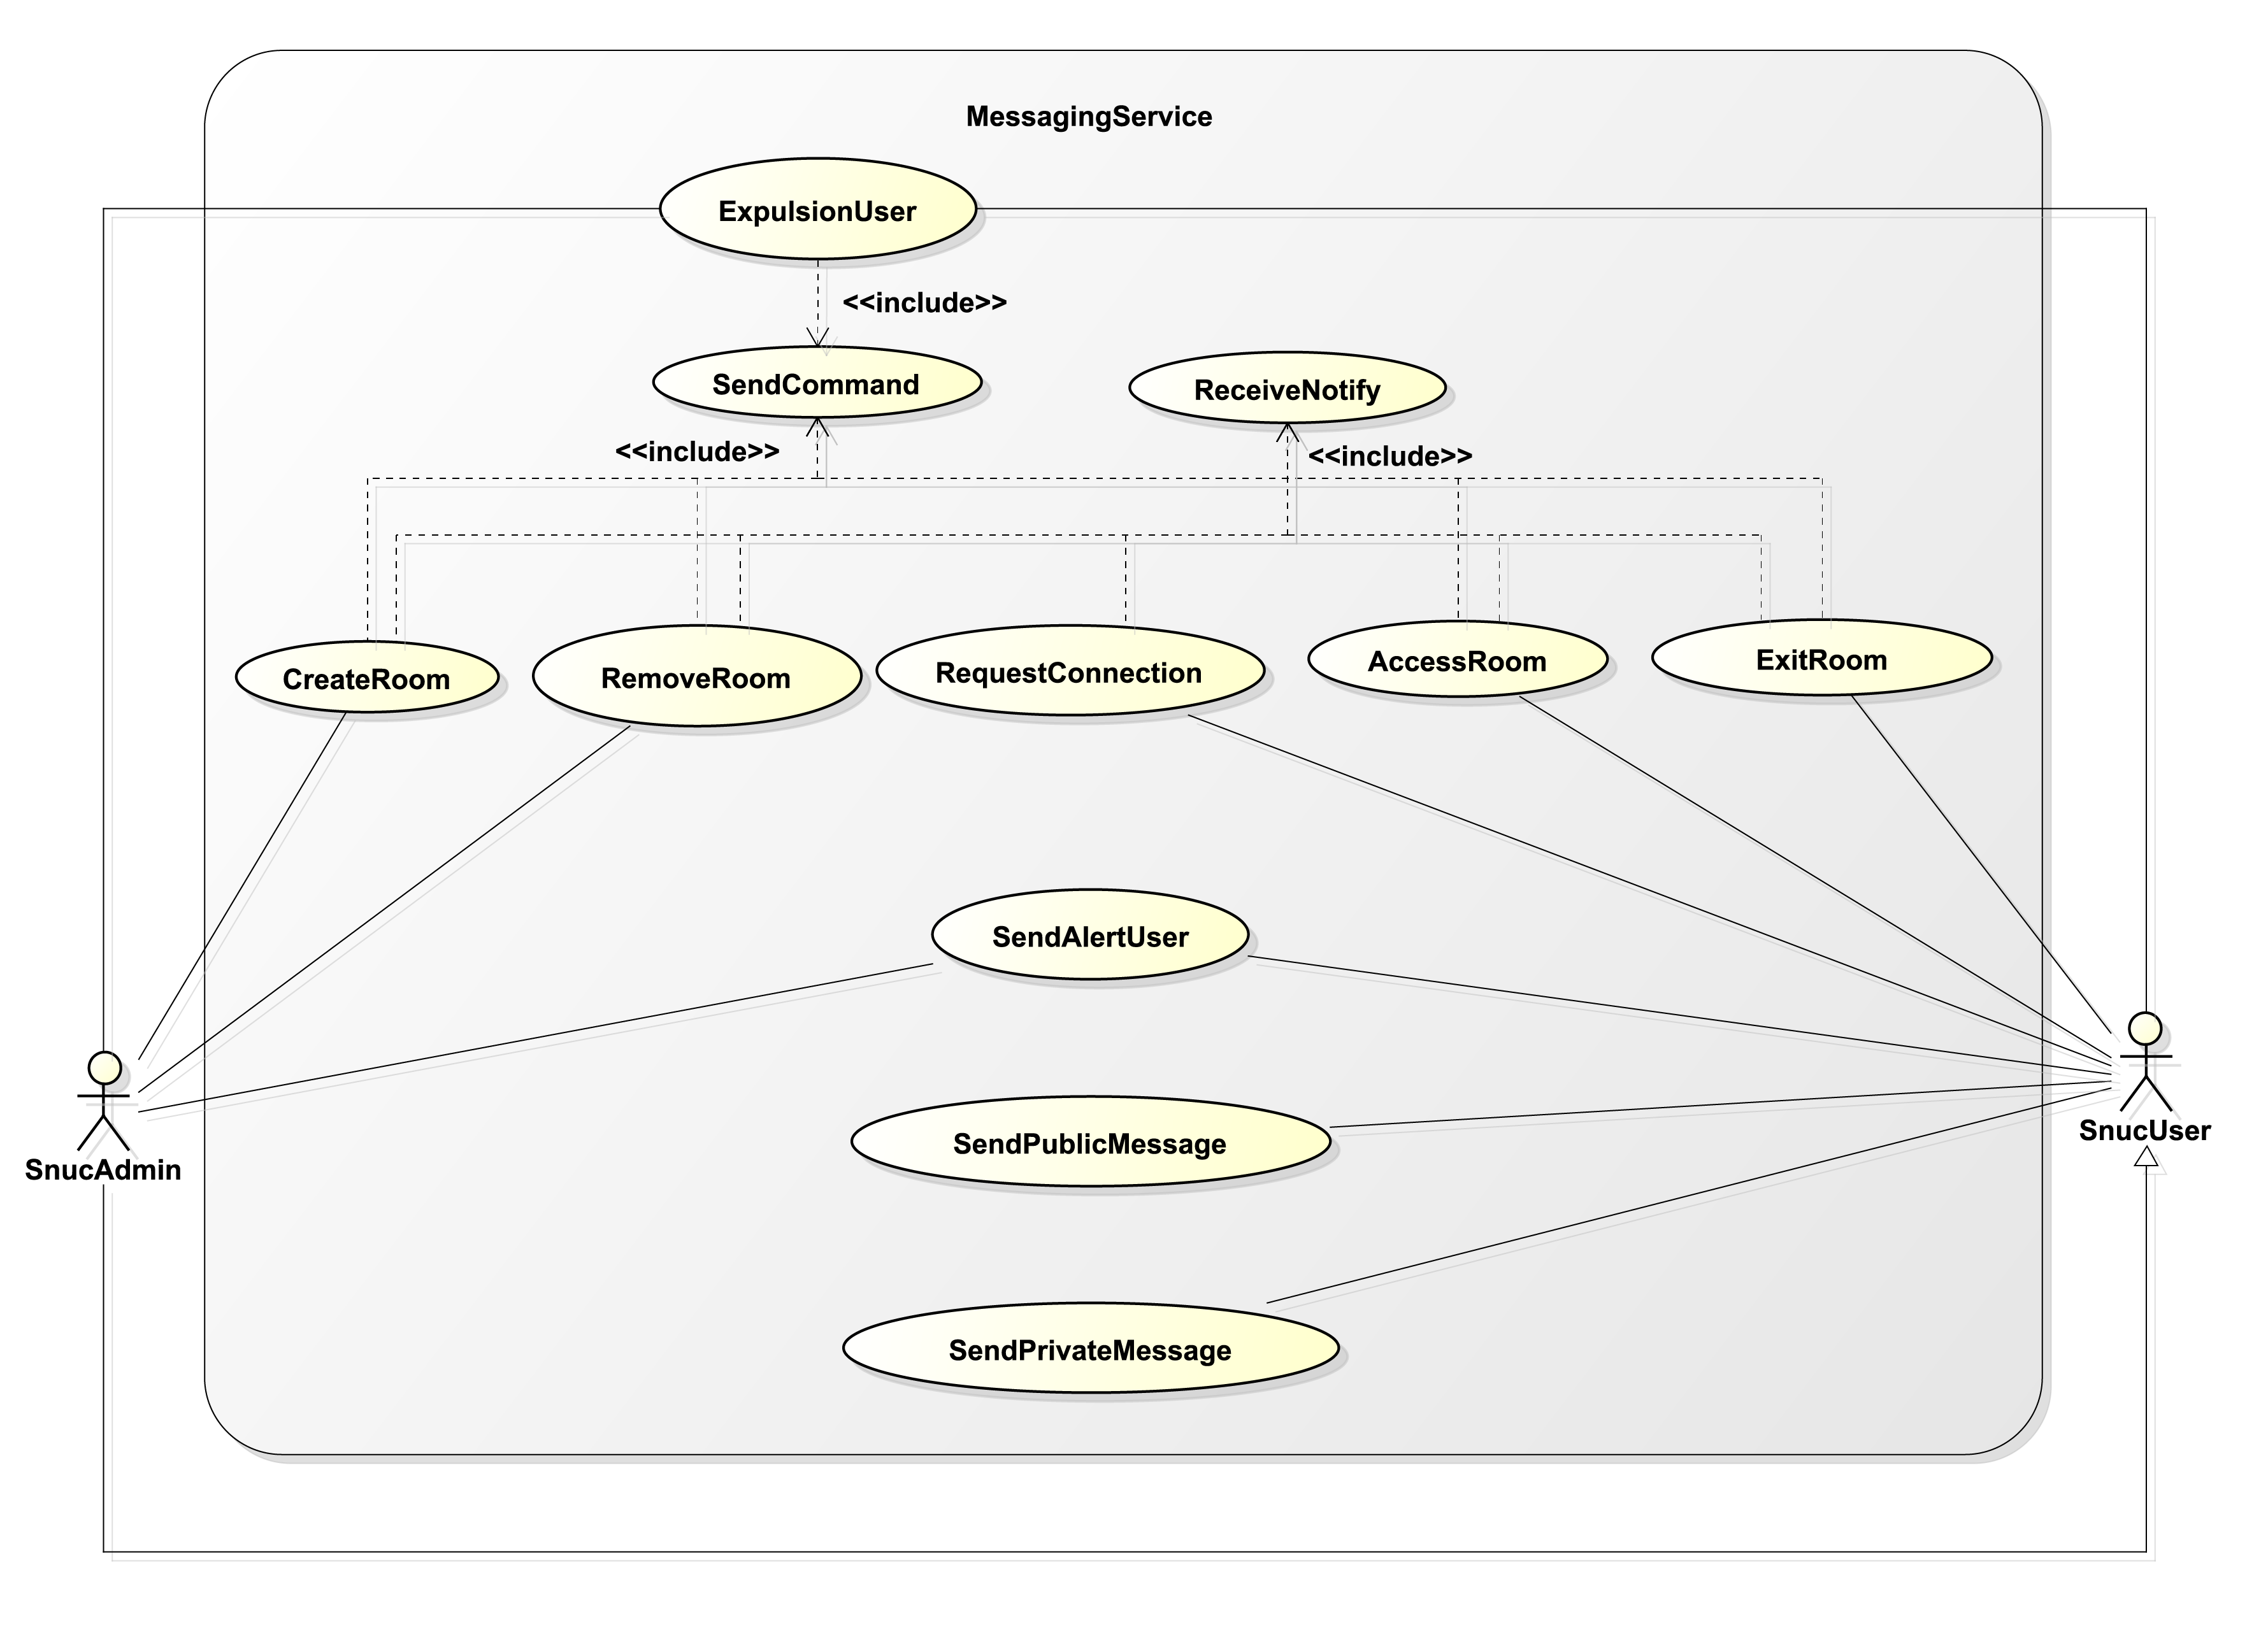
\includegraphics[scale=0.142]{image_astah/UseCaseDiagram.png}{\centering}
    \caption{Diagrammi dei casi uso} 
    \label{fig_UCD}
   \end{figure}
\end{frame}

\begin{frame} [allowframebreaks]
  \frametitle{Iterazione 1: Requisiti - Modello dei casi d'uso}
   \underline{Attori Identificati}: Amministratore (SnucAdmin) e Utente del Servizio di Messaggistica (SnucUser). \newline
   \underline{Casi d'uso identificati}: RequestConnection, AccessRoom, SendPublicMessage, SendPrivateMessage, ReceiveNotify, SendCommand, ExitRoom, CreateRoom, 
                                        RemoveRoom, SendAlertUser, ExpulsionUser. \newline
   Descrizione breve dei casi d'uso identificati:
   \begin{enumerate} 
    \item \textbf{RequestConnection}. L’utente si connette al sistema specificando il nickname, l’indirizzo e la porta del servizio di messaggistica.
    \item \textbf{AccessRoom}. L’utente richiede al sistema l’ingresso in una specifica stanza del servizio (che deve essere stata precedentemente creata 
          dall’amministratore del servizio). 
    \item \textbf{SendPublicMessage}. Il partecipante al servizio di messaggistica invia un messaggio ``pubblico'' che viene inviato dal sistema a tutti i 
          partecipanti che si trovano nella stessa stanza di colui che ha inviato il messaggio.
    \item \textbf{SendPrivateMessage}. Il partecipante al servizio di messaggistica  invia un messaggio ``privato'' ad uno specifico partecipante.
    \item \textbf{ExitRoom}. Un partecipante richiede al sistema l’uscita dal servizio. Questo comporta la sua eliminazione dall’insieme dei partecipanti presenti 
          nella stanza del servizio cui era precedentemente associato l’utente.
    \item \textbf{CreateRoom}. L’amministratore del servizio di messaggistica è responsabile della creazione delle stanze che potranno successivamente 
          essere visitate dai partecipanti.
    \item \textbf{RemoveRoom}. In ogni momento l’amministratore può eliminare una stanza dal servizio (ad esempio perchè non ci sono partecipanti). Ciò comporta 
          l’invio preventivo di un messaggio a tutti i patecipanti presenti nella stanza, i quali potranno in seguito richiedere l’ingresso in una   
          nuova stanza del servizio.
    \item \textbf{SendAlertUser}. L’amministratore può in ogni momento inviare un messaggio di avviso ad uno specifico partecipante al servizio.
    \item \textbf{ExpulsionUser}. L’amministratore può in ogni momento espellere da una stanza uno specifico partecipante.  
    \newline
    Descrizione breve dei sottocasi d'uso identificati:  
    \item \textbf{ReceiveNotify}. Il sistema manda dei messaggi di notifica, che permettono di aggiornare l’utente di un cambiamento dello stato del sistema.
    \item \textbf{SendCommand}. Il sistema è in grado di ricevere e interpretare dei comandi.
   \end{enumerate}
\end{frame}

\subsection{Iterazione 1: Requisiti - Glossario}
\setbeamertemplate{itemize items}[triangle]
\begin{frame} [allowframebreaks]
  \frametitle{Iterazione 1: Requisiti - Glossario} 
   \begin{itemize} 
    \item SnucUser, User, Utente: è l'utente del servizio di messaggistica che è in grado di registrarsi a delle stanze, di inviare messaggi pubblici e privati.
    \item SnucAdmin, Admin, Amministratore: è il gestore del servizio di messaggistica, che possiede la facoltà di creare e/o eliminare una stanza, di inviare un 
          particolare messaggio di avviso ad un partecipante per un comportamento non corretto ed eventualmente di bannarlo eliminandolo dalla stanza.
    \item Messaging Service, Servizio di messaggistica, sistema, chat: rappresenta ed incapsula il servizio di messaggistica nel suo complesso.
    \item Room, stanza, canale: rappresenta un luogo virtuale, dove gli utenti possono scambiarsi informazioni relative alle tematiche trattate.
    \item Messaggio Pubblico: messaggio testuale inviato da un partecipante a tutti gli utenti presenti nella stanza.
    \item Messaggio Privato: messaggio testuale inviato da un partecipante ad un particolare partecipante presente nella stanza.
    \item Notifica: particolare messaggi di avviso inviato dal server agli utenti che usufruiscono del servizio.  
  \end{itemize}
\end{frame}

\subsection{Iterazione 1: Requisiti - UC1\_RequestConnection}
\begin{frame}
 \frametitle{Iterazione 1: Requisiti - UC1\_RequestConnection}
  \begin{table}[!htbp]
     \caption {Descrizione dettagliata: caso d'uso UC1\_RequestConnection}
     \label{table_UC1_RC}
     \resizebox{\linewidth}{!}{%
      \begin{tabular}{|l|p{10cm}|}\hline
       Nome caso d'uso &  UC1\_RequestConnection \\\hline
       Portata & Applicazione Smart Network University Communications \\\hline
       Livello &  Obiettivo Utente \\\hline
       Attore primario &  SnucUser \\\hline
       Parti interessate e interessi &  SnucUser: vuole collegarsi al servizio di messaggistica \\\hline
       Pre-condizioni & L'utente ha bisogno di una connessione di rete\\\hline
       Post-condizioni (garanzia di successo) &  L'utente è inserito tra gli utenti online con il nickname confermato dal servizio di messaggistica ottenendo un 
                                                 messaggio di benvenuto \\\hline
       Scenario principale di successo &  
       \begin{enumerate} 
        \item L'utente inserisce un nickname, l'address e la porta del server.
        \item Il sistema esamina il nickname inviato dall'utente e verifica se è presente una omonimia.
        \item Il sistema conferma l'inserimento tra gli utenti online inviando una notifica di benvenuto.
       \end{enumerate} \\\hline
      \end{tabular}}
   \end{table}
\end{frame}

\begin{frame}
 \frametitle{Iterazione 1: Requisiti - UC1\_RequestConnection}
  \begin{table}[!htbp]
      \resizebox{\linewidth}{!}{%
       \begin{tabular}{|l|p{10cm}|}\hline
         Estensioni (o flussi alternativi) &  
           1A - SnucUser inserisce parametri errati: 
          \begin{itemize} 
           \item Viene visualizzato un messaggio di errore e viene richiesto nuovamente l’inserimento di tali parametri.
          \end{itemize} 
           2A - Omonimia del nickname:
          \begin{itemize}       
           \item Il sistema cambia il nickname aggiungendo il carattere ``"\_"'' al nickname (es. \_nickname). 
           \item Il sistema conferma l'inserimento tra gli utenti online inviando una notifica di benvenuto.
          \end{itemize} \\\hline
       Requisiti speciali (Requisiti Non Funzionali) &  Comunicazione asincrona in cui lo scambio di informazioni avviene in tempo reale, senza sensibili pause tra 
                                                        invio e ricezione del messaggio.\\\hline
       Elenco delle varianti tecnologiche &  L’applicazione dovrebbe essere flessibile al funzionamento di diversi protocolli di comunicazione (es. TCP, UDP) e con   
       diversi strati middleware (es. Socket, RMI) \\\hline
       Frequenza di ripetizione & Potrebbe essere quasi ininterrotta \\\hline
       Varie e/o Problemi Aperti &  // \\\hline
      \end{tabular}}
   \end{table}
\end{frame}

\subsection{Iterazione 1: Requisiti - UC2\_AccessRoom}
\begin{frame}
 \frametitle{Iterazione 1: Requisiti - UC2\_AccessRoom}
  \begin{table}[!htbp]
   \caption {Caso d'uso UC2\_AccessRoom}
    \label{table_UC2_AR}
     \resizebox{\linewidth}{!}{%
      \begin{tabular}{|l|p{10cm}|}\hline
       Nome caso d'uso &  UC2\_AccessRoom\\\hline
       Portata & Applicazione Smart Network University Communications \\\hline
       Livello & Obiettivo Utente \\\hline
       Attore primario & SnucUser  \\\hline
       Parti interessate e interessi & SnucUser: vuole registrarsi e effettuare l’ingresso in una stanza presente nel servizio di messaggistica \\\hline
       Pre-condizioni & Nel sistema è presente almeno una stanza creata da un amministratore.\\\hline
       Post-condizioni (garanzia di successo) &  Nel caso di svolgimento normale l’utente è registrato ed è presente nell’insieme degli utenti della stanza 
                                                 specificata. \\\hline
      \end{tabular}}
   \end{table}
\end{frame}

\begin{frame}
 \frametitle{Iterazione 1: Requisiti - UC2\_AccessRoom}
  \begin{table}[!htbp]
      \resizebox{\linewidth}{!}{%
       \begin{tabular}{|l|p{10cm}|}\hline
          Scenario principale di successo &  
           \begin{enumerate} 
            \item L’utente richiede una lista di stanze presenti nel sistema  di messaggistica.
            \item Il sistema invia la lista delle stanze.
            \item L’utente seleziona la stanza tra quelle presenti in lista.
            \item Il sistema registra l’utente alla stanza.
            \item Il sistema visualizza a video gli utenti presenti nella stanza.
            \item Il sistema visualizza un’area pubblica dove vengono mostrati tutte le conversazioni in corso dal quel momento in poi. 
          \end{enumerate} \\\hline 
         Estensioni (o flussi alternativi) &  
           3A - Il SnucUser inserisce una stanza non in elenco:
          \begin{enumerate} 
           \item Il sistema invia un messaggio di errore.
          \end{enumerate} \\\hline
       Requisiti speciali (Requisiti Non Funzionali) &  Comunicazione asincrona in cui lo scambio di informazioni avviene in tempo reale, senza sensibili pause tra 
                                                        invio e ricezione del messaggio.\\\hline
       Elenco delle varianti tecnologiche &  L’applicazione dovrebbe essere flessibile al funzionamento di diversi protocolli di comunicazione (es. TCP, UDP) e con   
       diversi strati middleware (es. Socket, RMI) \\\hline
       Frequenza di ripetizione & Potrebbe essere quasi ininterrotta \\\hline
       Varie e/o Problemi Aperti &  // \\\hline
      \end{tabular}}
   \end{table}
\end{frame}

\begin{frame}{Descrizione Prototipo User Interface}
 Viene presentata un prototipo dell'interfaccia grafica (GUI) al cliente realizzata tramite Balsamiq Mockups per rendere più visibile 
 il confine del sistema di iterazione da parte delle figure coinvolte con l'ipotetico sistema da realizzare, in modo da sollevare
 ipotetiche situazioni problematiche relative. 
\end{frame} 

\begin{frame} {Iterazione 1: Requisiti - Prototipo  User Interface}
    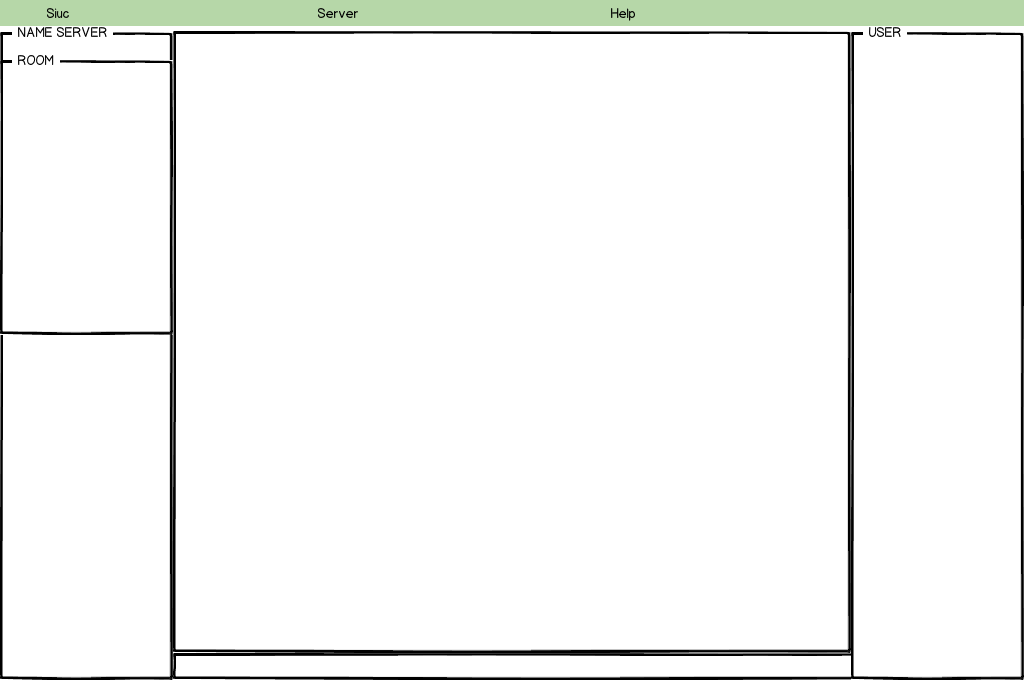
\includegraphics[scale=0.28]{image_mockups/01_snuc_open.png}{\centering}
\end{frame}

\begin{frame} {Iterazione 1: Requisiti - Prototipo User Interface}
    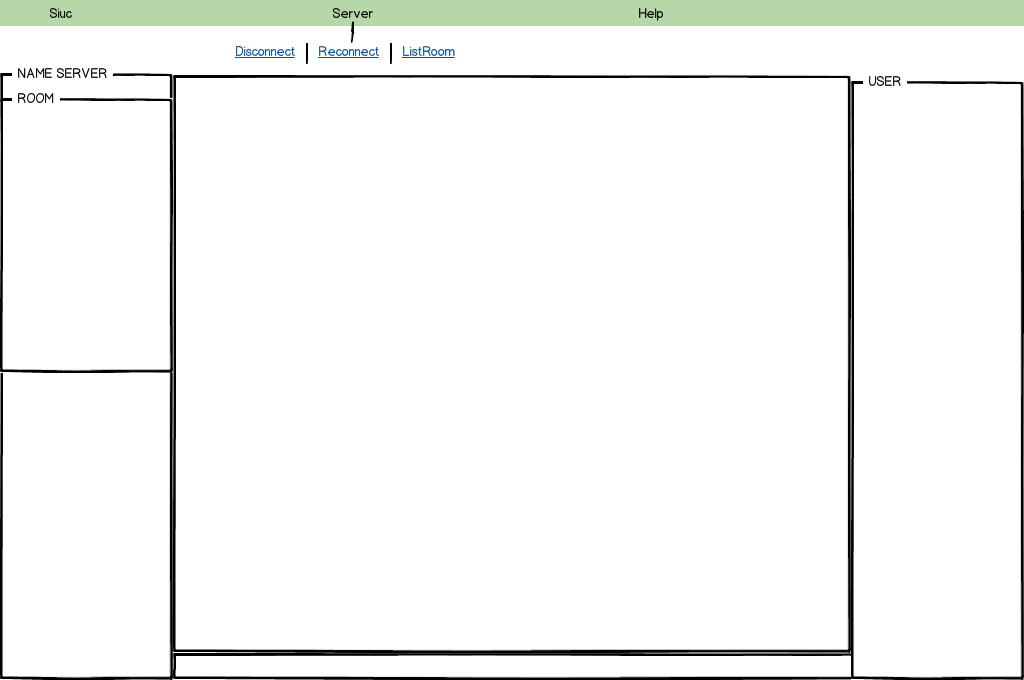
\includegraphics[scale=0.28]{image_mockups/02_snuc_menu_server.png}{\centering}
\end{frame}

\begin{frame} {Iterazione 1: Requisiti - Prototipo User Interface}
    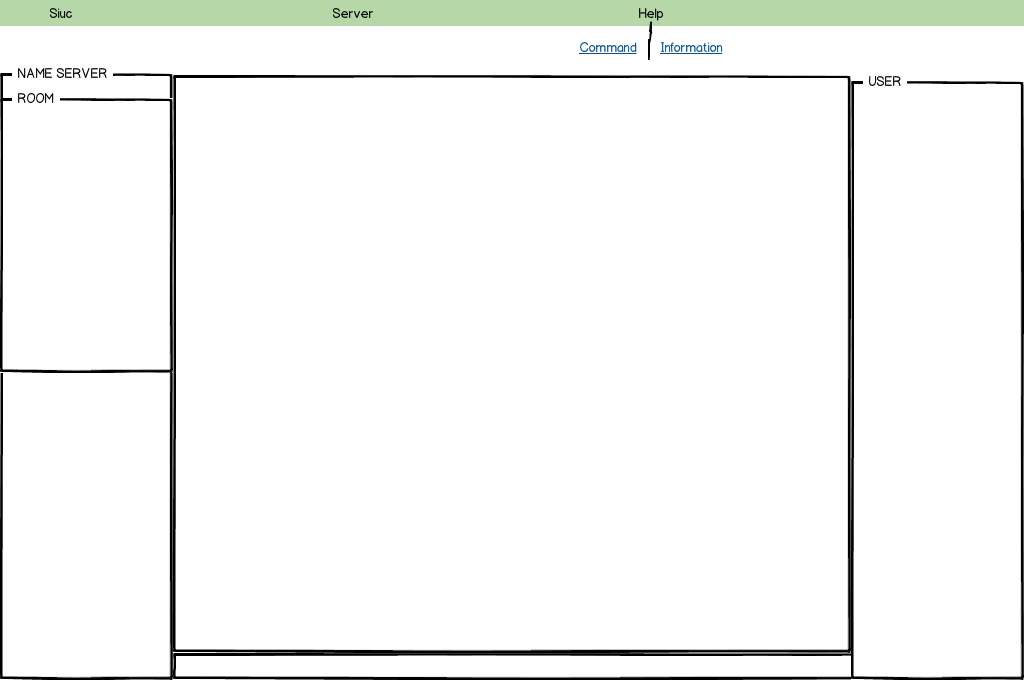
\includegraphics[scale=0.28]{image_mockups/03_snuc_menu_help.png}{\centering}
\end{frame}

\begin{frame} {Iterazione 1: Requisiti - Prototipo User Interface}
    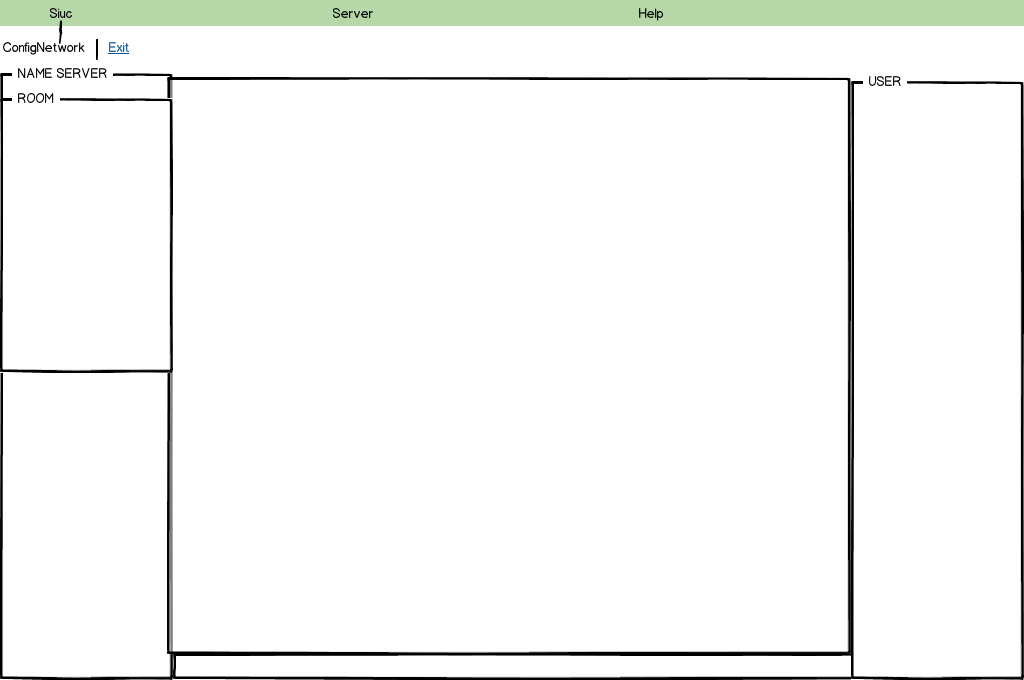
\includegraphics[scale=0.28]{image_mockups/04_snuc_menu_snuc.png}{\centering}
\end{frame}

\begin{frame} {Iterazione 1: Requisiti - Prototipo User Interface}
    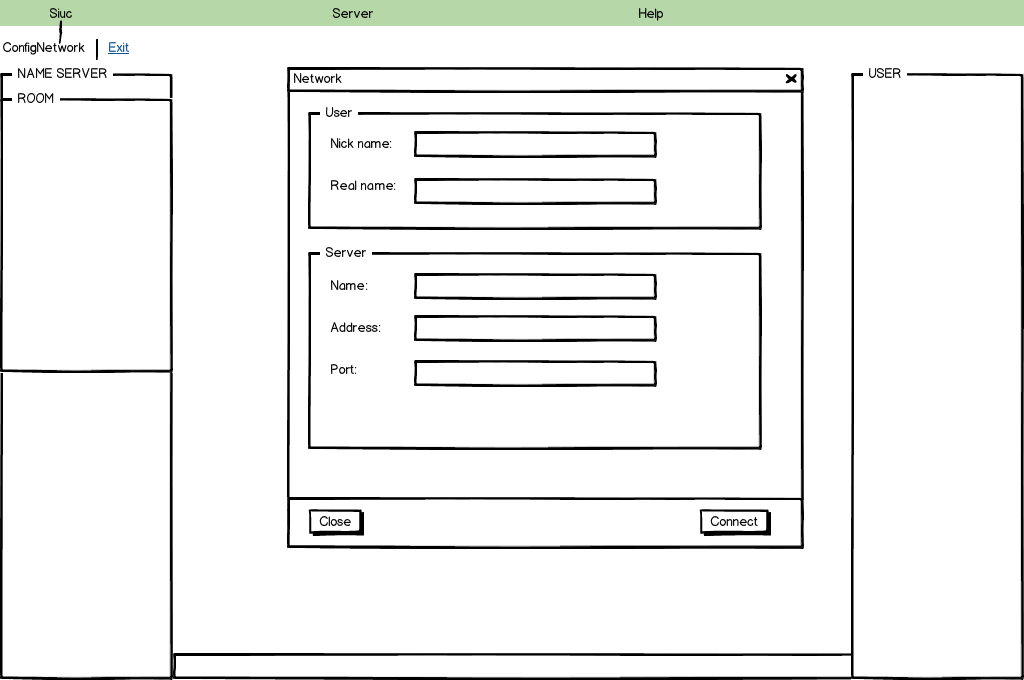
\includegraphics[scale=0.28]{image_mockups/05_snuc_config_network.png}{\centering}
\end{frame}

\begin{frame} {Iterazione 1: Requisiti - Prototipo User Interface}
    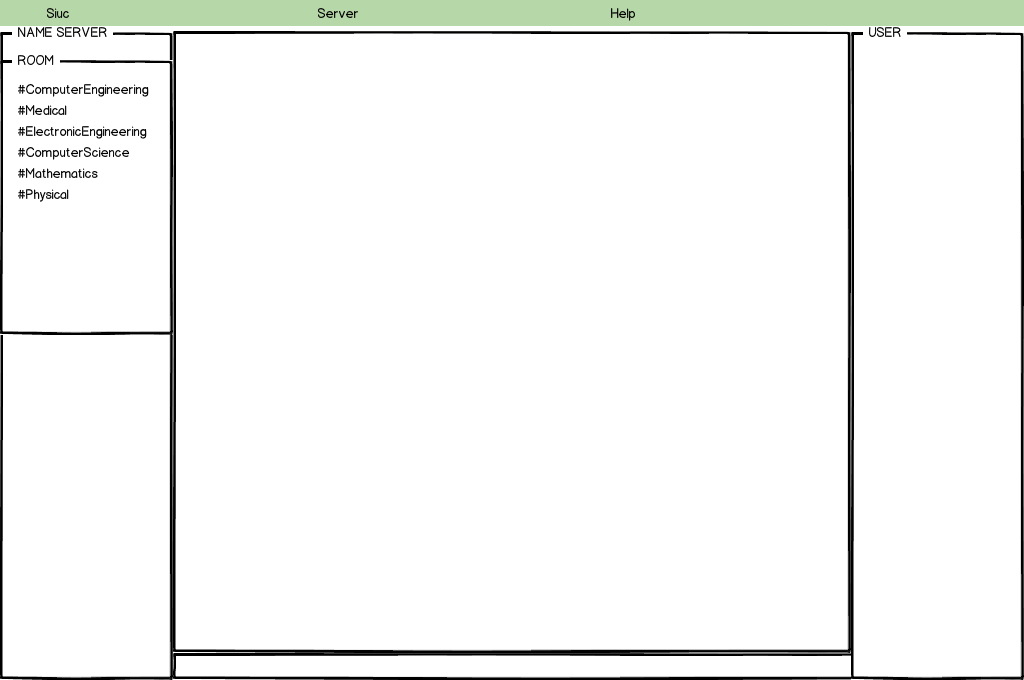
\includegraphics[scale=0.28]{image_mockups/06_snuc_connect.png}{\centering}
\end{frame}

\begin{frame} {Iterazione 1: Requisiti - Prototipo User Interface}
    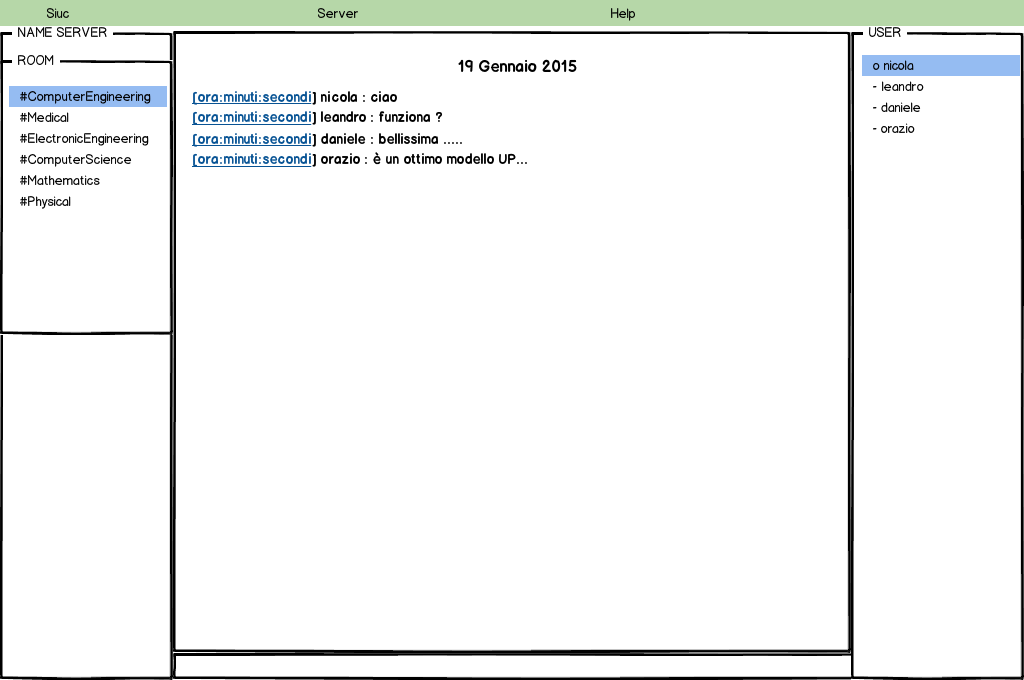
\includegraphics[scale=0.28]{image_mockups/07_snuc_user_room_ce.png}{\centering}
\end{frame}

\begin{frame} {Iterazione 1: Requisiti - Prototipo User Interface}
    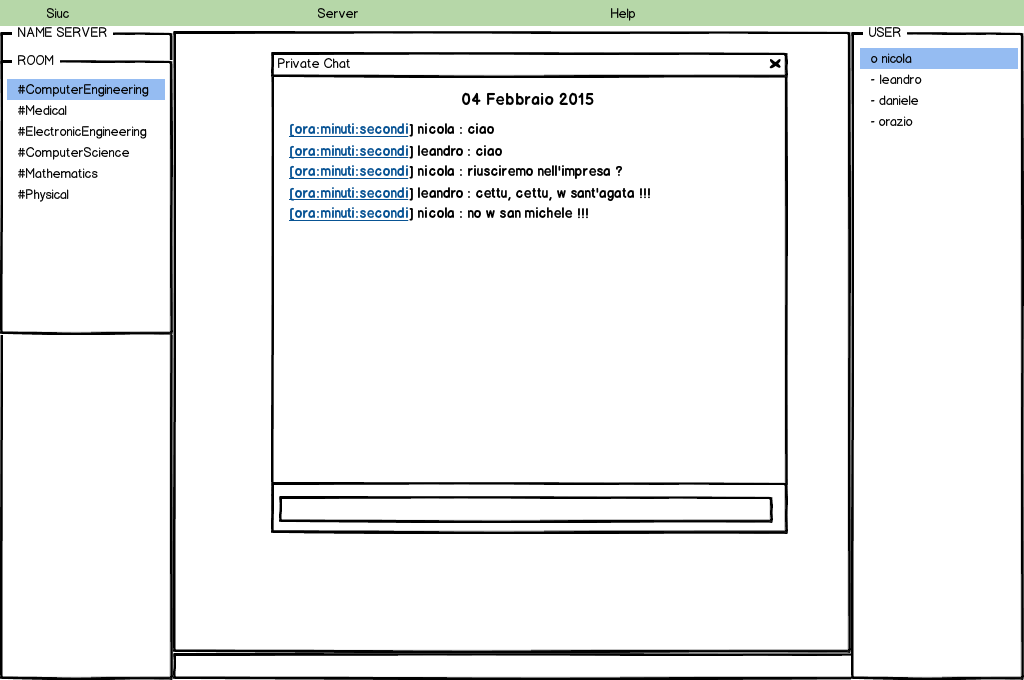
\includegraphics[scale=0.28]{image_mockups/08_snuc_user_room_ce_private.png}{\centering}
\end{frame}

\begin{frame} {Iterazione 1: Requisiti - Prototipo User Interface}
    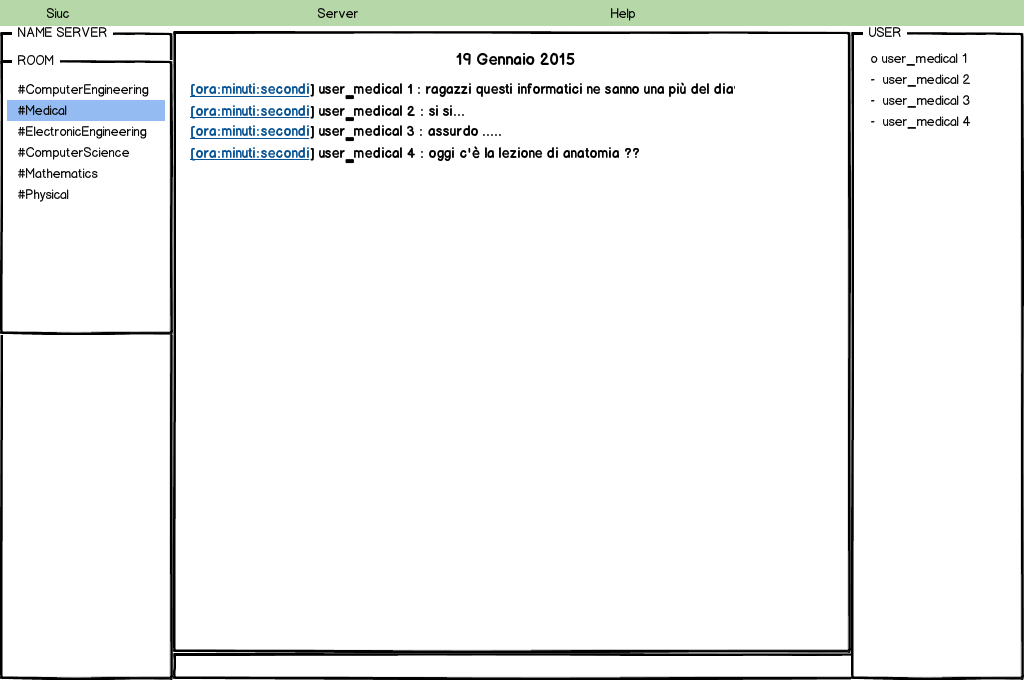
\includegraphics[scale=0.28]{image_mockups/09_snuc_user_room_medical.png}{\centering}
\end{frame}

% ANALISI ITERAZIONE 1 - UC1_RequestConnection e UC2_AccessRoom
\subsection{Iterazione 1: Analisi - UC1\_RequestConnection}
\begin{frame}[allowframebreaks] {Descrizione Analisi - UC1\_RequestConnection}
 In questa iterazione, del caso d’uso UC1 è di interesse lo scenario principale di successo.  Da esso è possibile identificare le seguenti classi concettuali: 	
 \begin{itemize}
  \item \textbf{User}: rappresenta il generico utente connesso al servizio di messaggistica. È caratterizzato da un ``nickname'' e può ricevere notifiche dal sistema 
                centrale.
  \item \textbf{MessagingService}: rappresenta ed incapsula il servizio di messaggistica nel suo complesso. Mantiene una lista di utenti connessi a tale sistema.
  \item \textbf{Message}: individua un generico messaggio scambiato tra utenti della chat o tra servizio di messaggistica e utente. È costituito da un 
               ``content'' (contenuto del messaggio), da una ``date'' (rappresenta la data) e dal ``sender'' (mittente).
  \item \textbf{Notify}: è una specializzazione del tipo Message ed è caratterizzata da un ``typeNotify'' che serve a distinguere il tipo di notifica (ad es. 
        CONNECTION\_ACCEPT nel caso in cui la connessione è stata stabilita correttamente).        
 \end{itemize}
\end{frame}

\begin{frame} {Iterazione 1: Analisi - UC1\_RequestConnection}
   \begin{figure}
     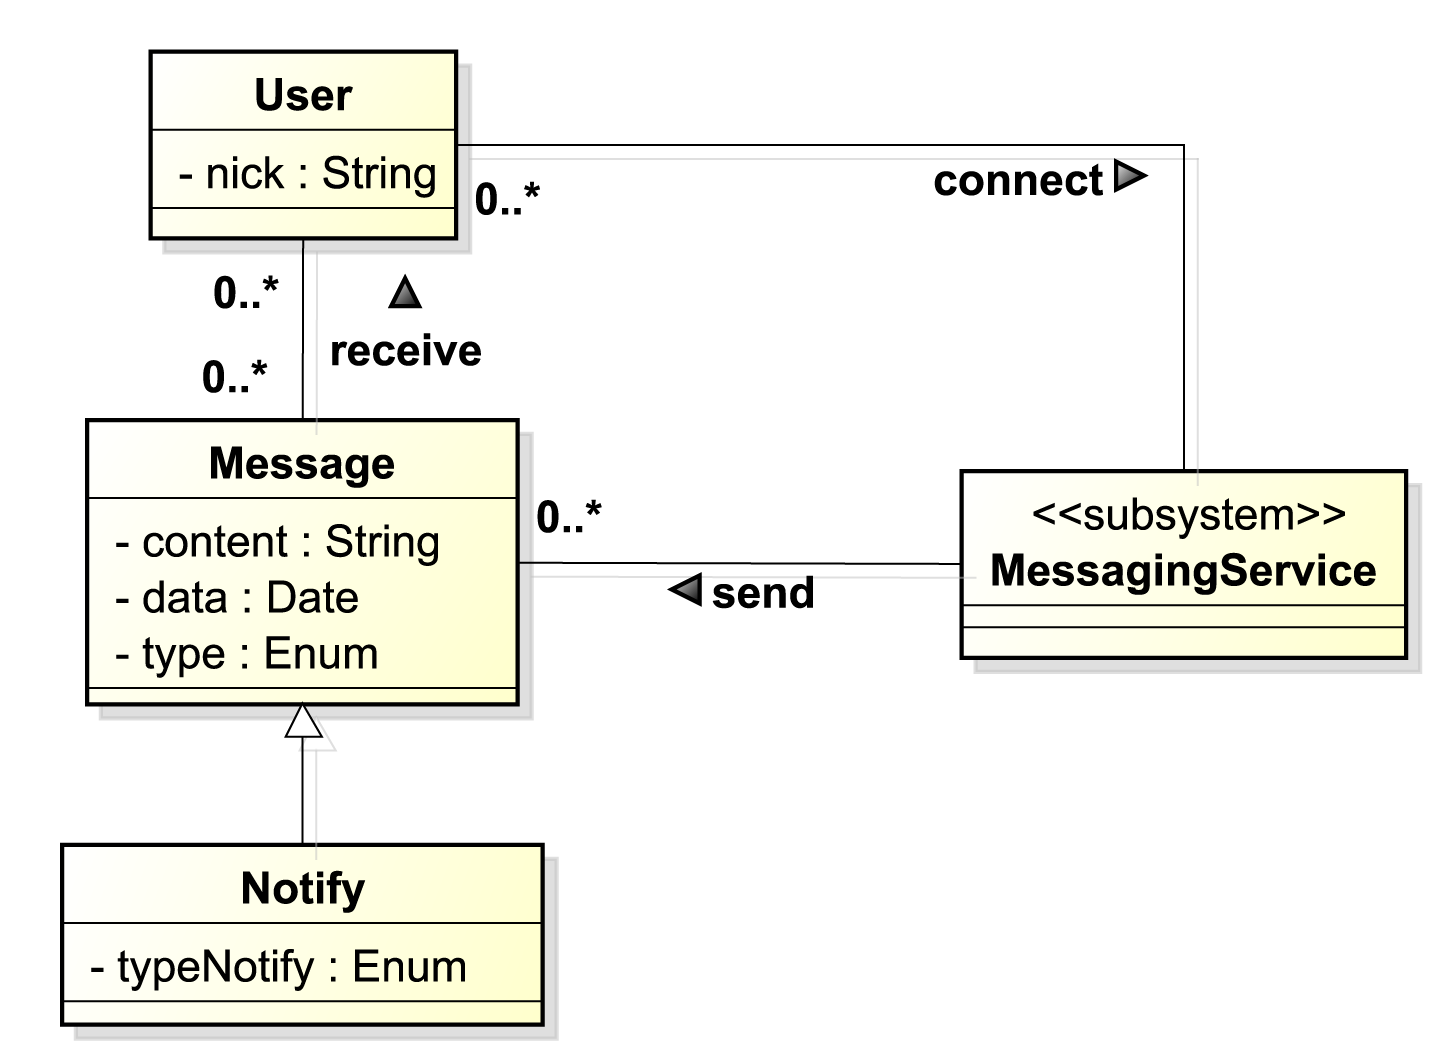
\includegraphics[scale=0.34]{image_astah/Iteration_1_DomainModel/UC1_RequestConnection_DM.png}{\centering}
     \caption{UC1 - Modello di dominio}
     \label{fig_UC1_RC_DM} 
   \end{figure}
\end{frame}

\begin{frame} {Iterazione 1: Analisi - UC1\_RequestConnection}
   \begin{figure}
     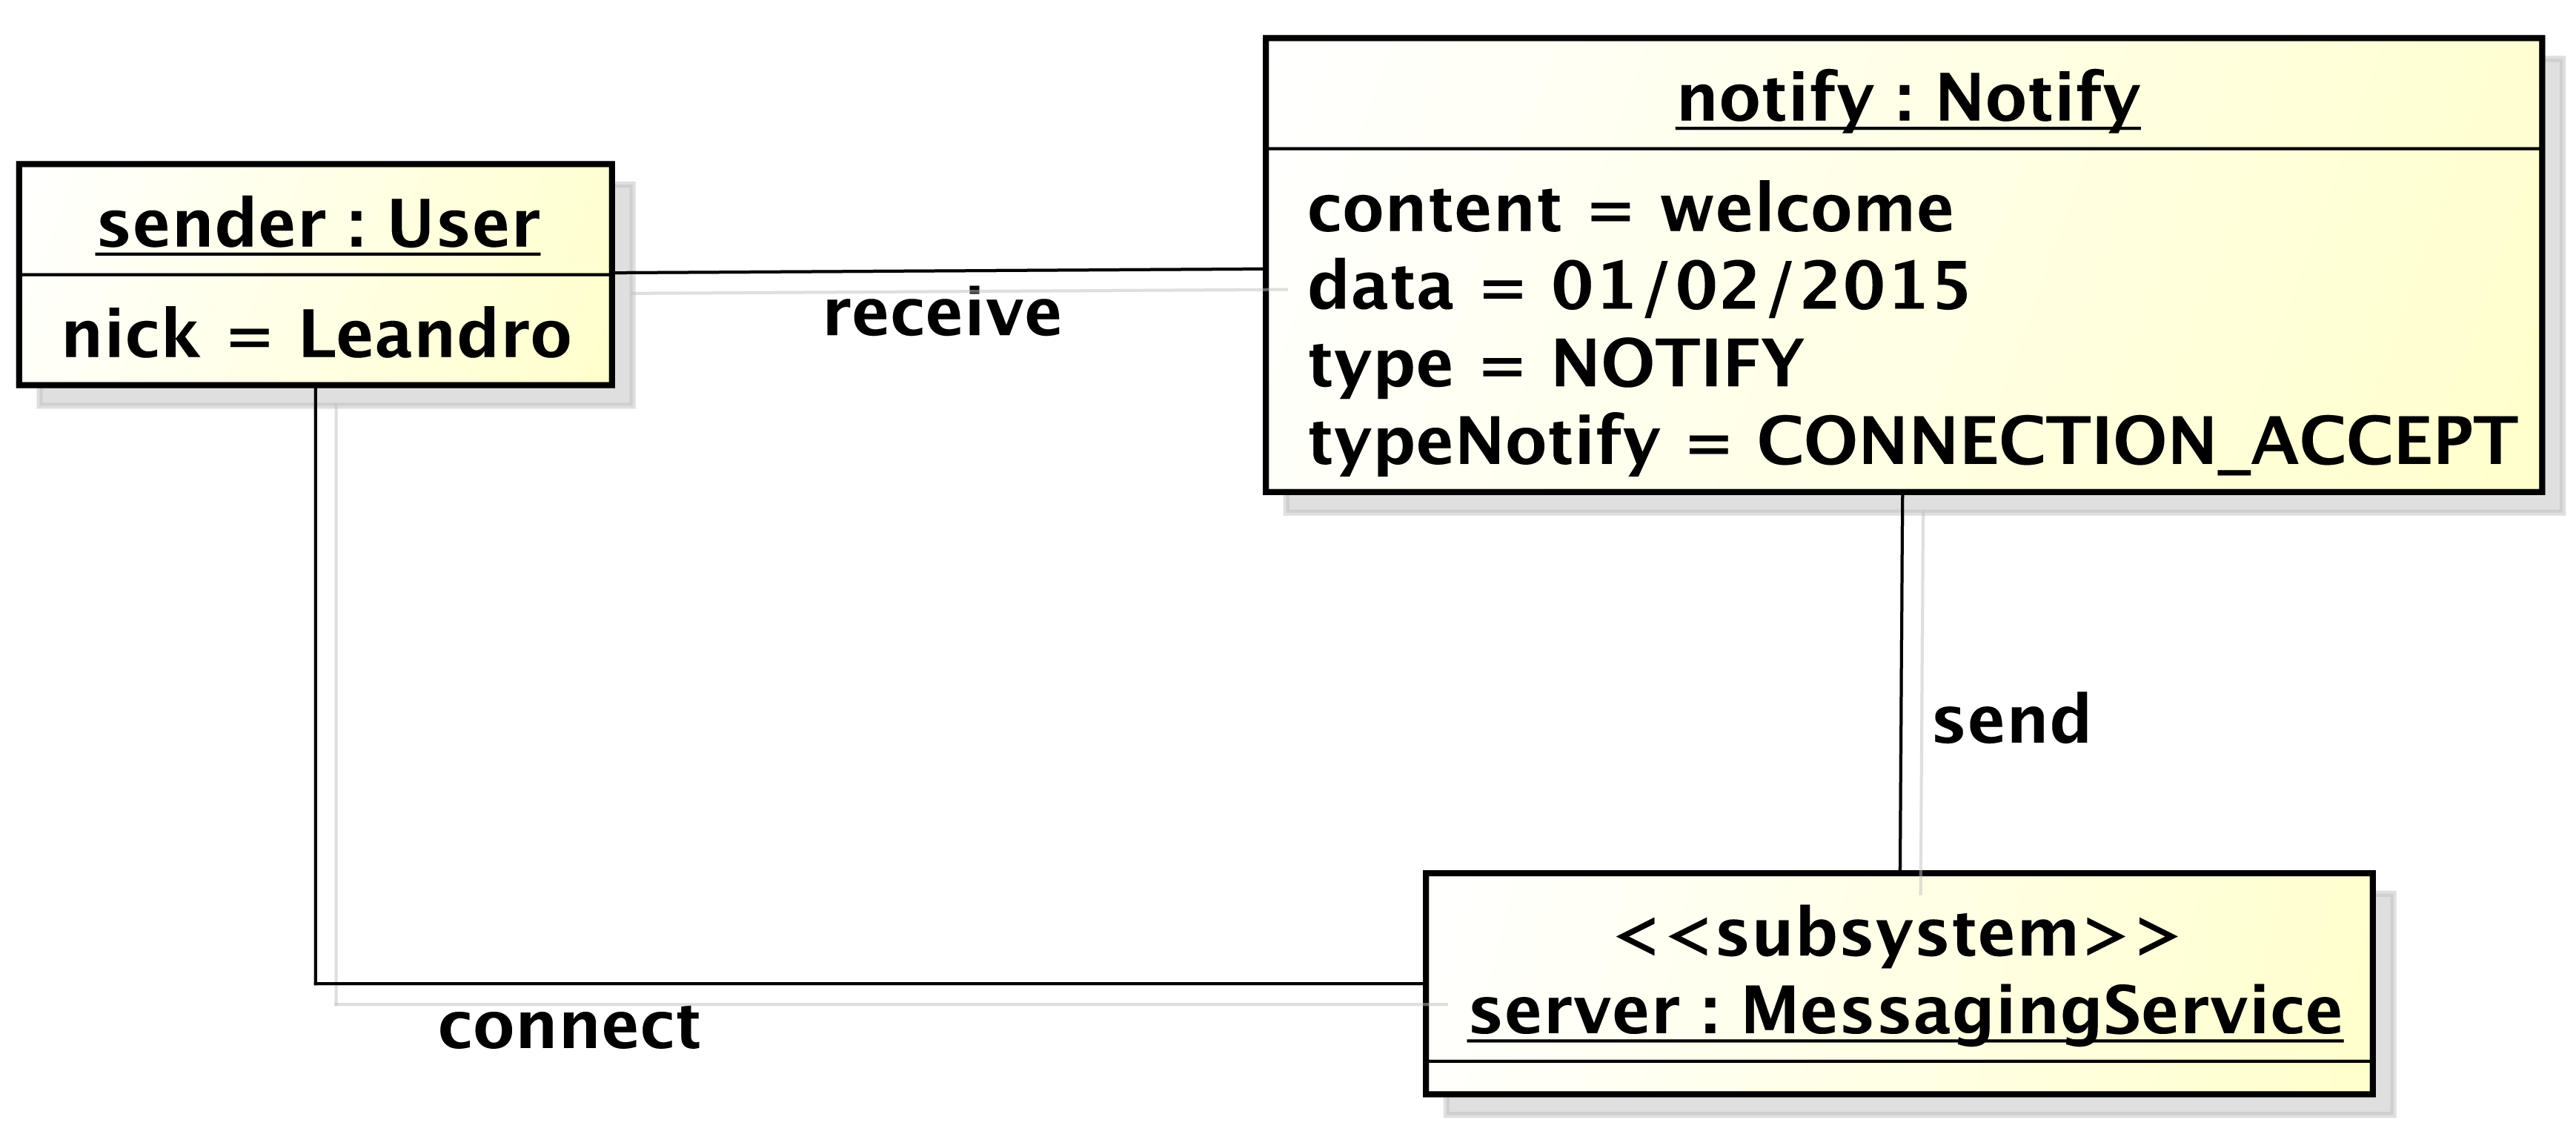
\includegraphics[scale=0.35]{image_astah/Iteration_1_DomainModel/UC1_RequestConnection_OM}{\centering}
     \caption{UC1 - Oggetti di dominio}
     \label{fig_UC1_RC_OM} 
   \end{figure}
\end{frame}

\begin{frame} {Iterazione 1: Analisi - UC1\_RequestConnection}
   \begin{figure}
     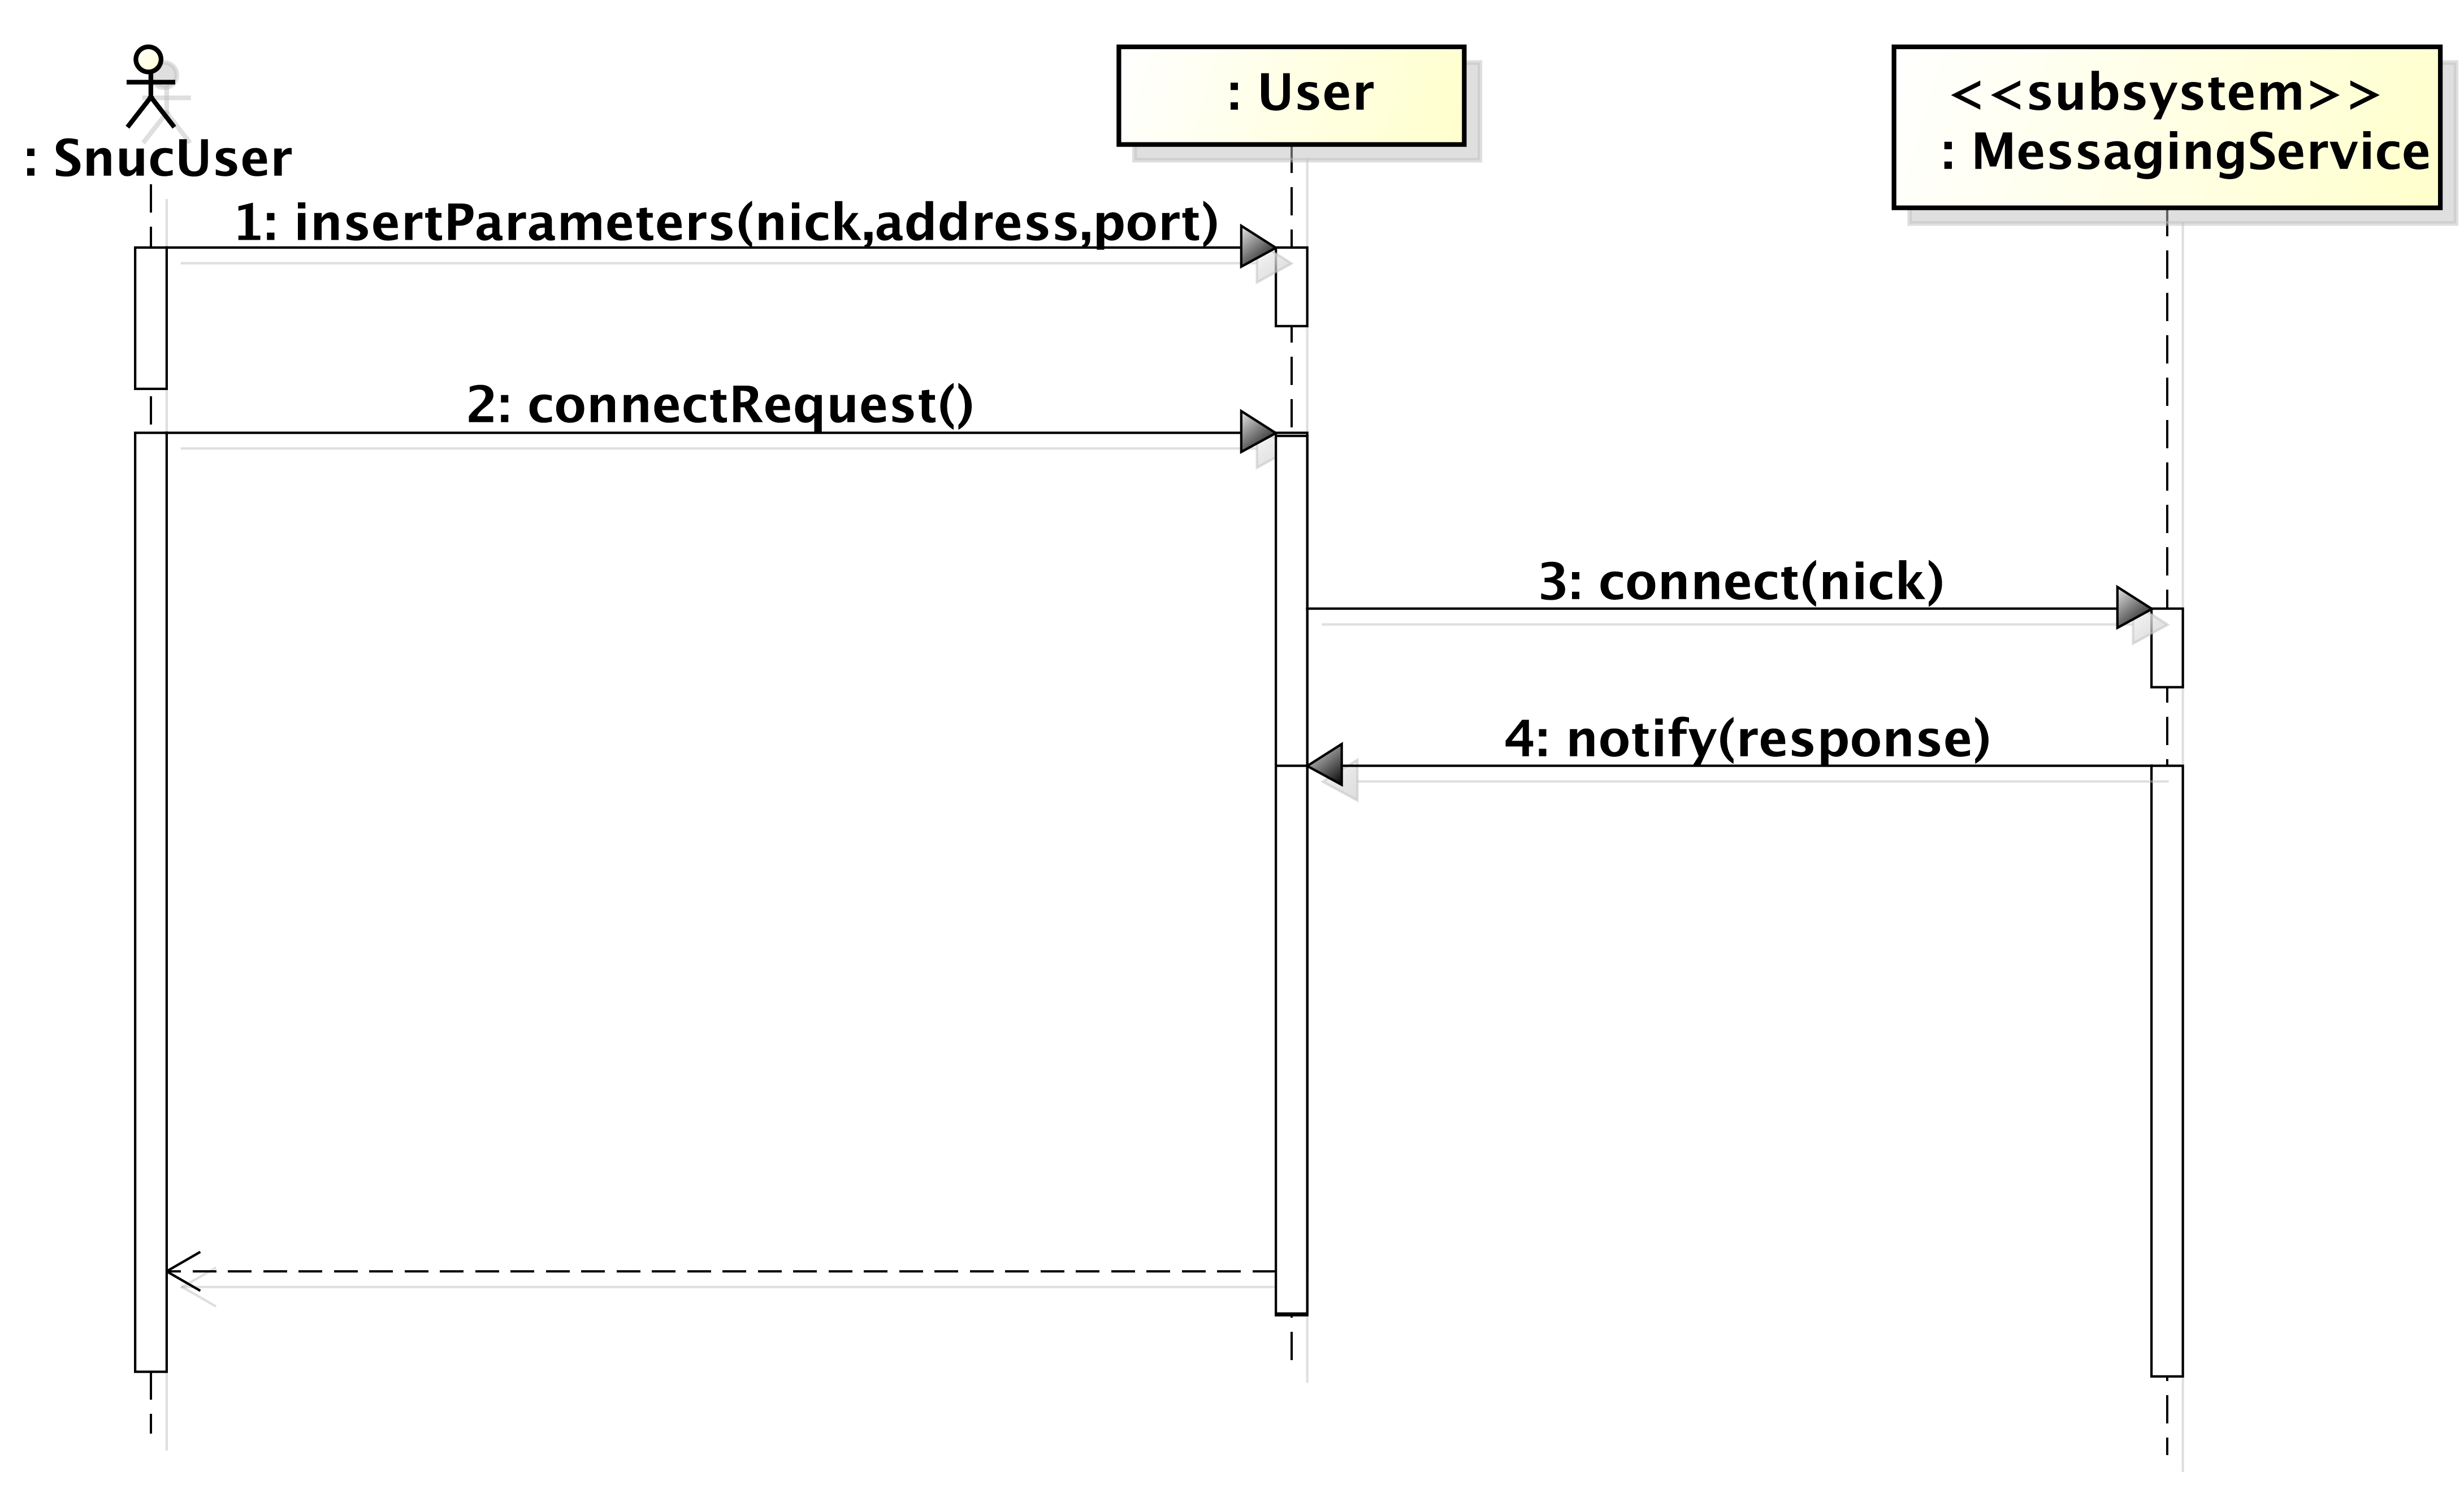
\includegraphics[scale=0.27]{image_astah/Iteration_1_DomainModel/UC1_RequestConnection_SSD.png}{\centering}
     \caption{UC1 - Diagramma di sequenza di dominio}
     \label{fig_UC1_RC_SSD} 
   \end{figure}
\end{frame}

\begin{frame}
 \frametitle{Iterazione 1: Analisi - UC1 contratti CO1/CO2}
  \begin{table}[!htbp]
   \caption {UC1 Contratto CO1 - connect}
    \label{table_CO1}
      \resizebox{\linewidth}{!}{%
       \begin{tabular}{|l|p{10cm}|}\hline
         Operazione & \textit{connect(nick: String)}  \\\hline 
         Riferimenti &  Caso d'uso: UC1\_RequestConnection \\\hline
         Pre-condizione & L'utente ha inserito correttamente i parametri di connessione (``address'' e ``port'') \\\hline 
         Post-condizione & L'utente è connesso al servizio di messaggistica e viene aggiunto nella lista degli utenti online \\\hline
      \end{tabular}}
   \end{table}
  \begin{table}[!htbp]
   \caption {UC1 Contratto CO2 - notify}
    \label{table_CO2}
      \resizebox{\linewidth}{!}{%
       \begin{tabular}{|l|p{10cm}|}\hline
         Operazione & \textit{notify(n: Notify)} \\\hline 
         Riferimenti &  Caso d'uso: UC1\_RequestConnection \\\hline
         Pre-condizione & L'utente è connesso al servizio di messaggistica \\\hline 
         Post-condizione & L'utente riceve la notifica \\\hline
      \end{tabular}}
   \end{table}

\end{frame}

\subsection{Iterazione 1: Analisi - UC2\_AccessRoom}
\begin{frame} [allowframebreaks] {Descrizione Analisi - UC2\_AccessRoom}
  In questa iterazione, del caso d’uso UC2 è di interesse lo scenario principale di successo.  Da esso è possibile identificare le seguenti classi concettuali: 
  \begin{itemize}
    \item \textbf{User}: rappresenta il generico utente, caratterizzato da un ``nickname'', connesso al servizio di messaggistica. \textit{Può richiedere la lista 
     delle stanze, ricevere notifiche dal sistema centrale. Interagisce con il MessagingSevice richiedendo la registrazione e l'ingresso in una specifica stanza}.
    \item \textbf{MessagingService}: rappresenta ed incapsula il servizio di messaggistica nel suo complesso. Mantiene una lista di utenti connessi a tale 
    sistema. \textit{Mantiene una lista di stanze e riceve tramite comandi richieste di ingresso da parte degli utenti}.
    \item \textbf{Message}: individua un generico messaggio scambiato tra utenti della chat o tra servizio di messaggistica e utente. È costituito da un ``content'' 
          (contenuto del messaggio), da una ``date'' (rappresenta la data) e dal ``sender'' (mittente).
    \item \textbf{Notify}: è una specializzazione del tipo Message ed è caratterizzata da un typeNotify che serve a distinguere il tipo di notifica (ad es. 
          CONNECTION\_ACCEPT nel caso in cui la connessione è stata stabilita correttamente, \textit{BAD\_COMMAND nel caso in cui il comando inviato dall'User non 
          sia riconosciuto dal Server)}.
    \item \textit{\textbf{PublicNotify}: è una specializzazione di Notify e questo tipo di notifica viene ricevuta da tutti gli utenti registrati alla relativa 
          stanza. Un esempio di PublicNotify è la notifica caratterizzata dal seguente typeNotify: UPDATE\_LIST\_USERS, grazie alla quale viene 
          aggiornata la lista degli utenti registrati nella relativa stanza}.
   \item  \textit{\textbf{Commad}: è una specializzazione di Message e rappresenta il comando che viene inviato dall'User e ricevuto ed interpretato dal            
          MessagingService (es. /join '\#Medical'  è richiesta da parte dell'utente a registrarsi alla stanza Medical)}.        
    \item \textit{\textbf{Room}: è caratterizzata da un nome. Ciascuna istanza individua una specifica stanza nella chat}.
    \item \textit{\textbf{Register}: mantiene un riferimento all’insieme di partecipanti che in un certo istante sono presenti nella stanza}.
   \end{itemize}
\end{frame}

\begin{frame} {Iterazione 1: Analisi - UC2\_AccessRoom}
   \begin{figure}
     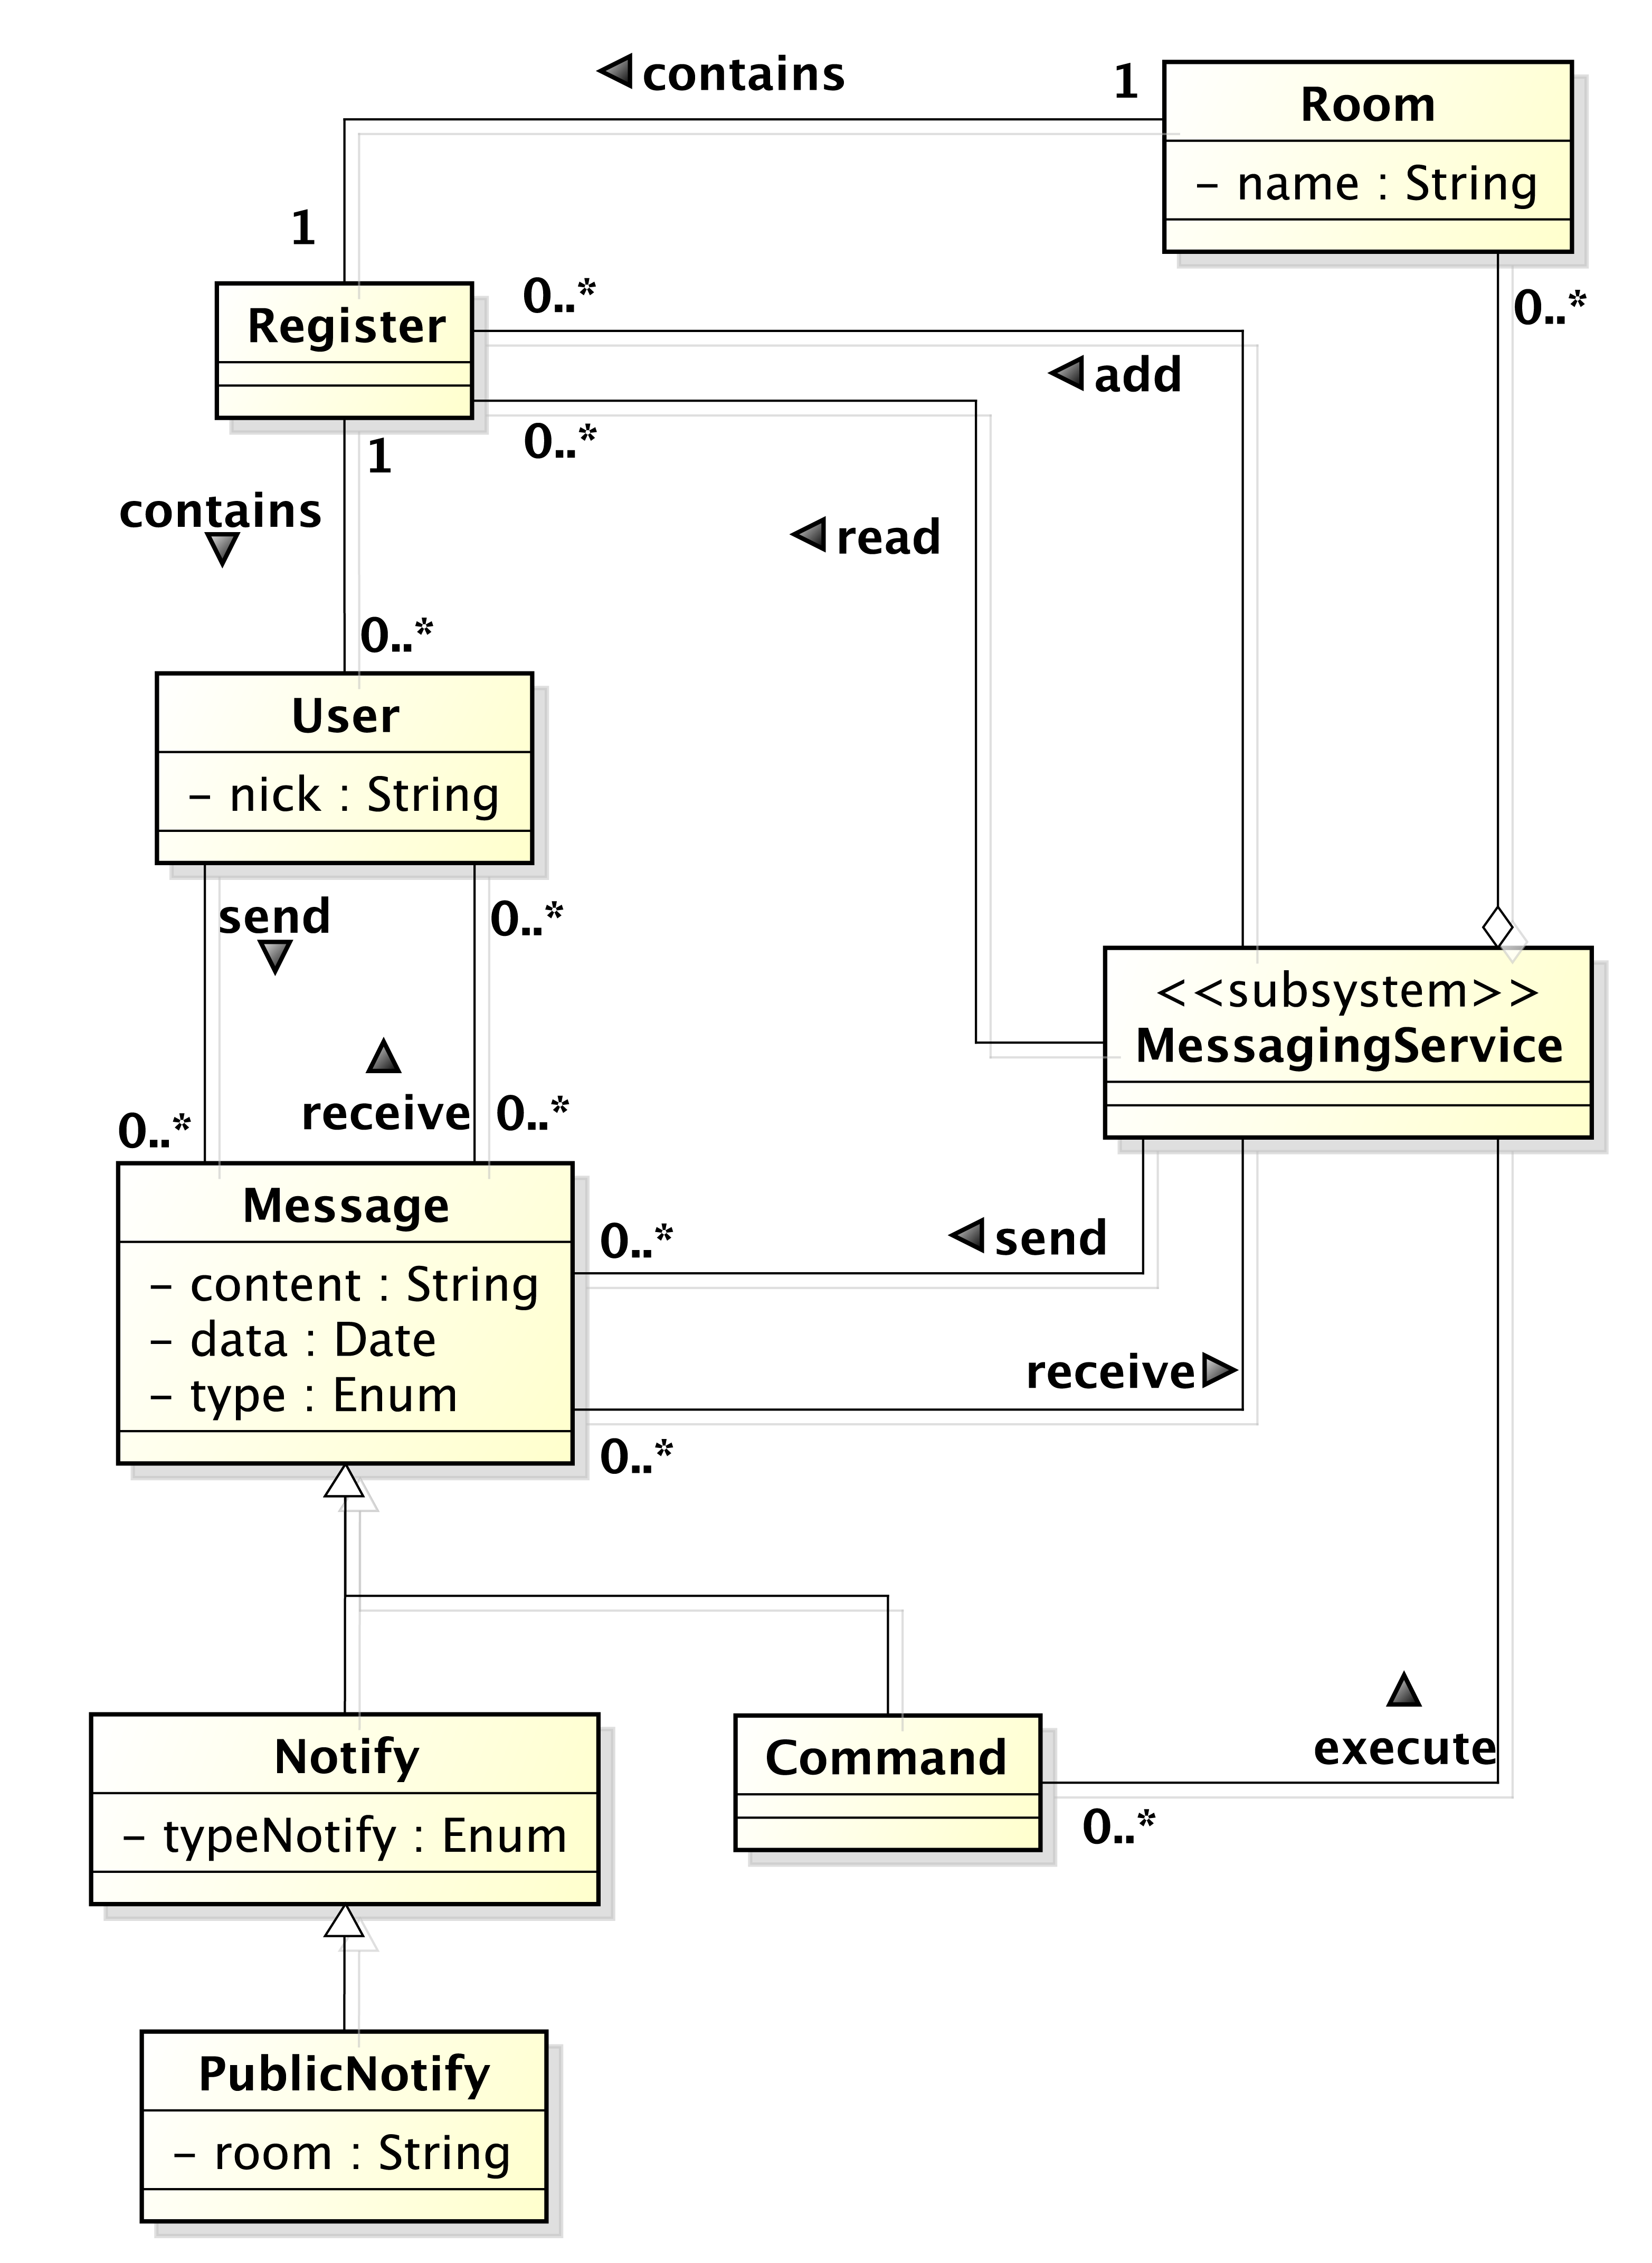
\includegraphics[scale=0.165]{image_astah/Iteration_1_DomainModel/UC2_AccessRoom_DM.png}{\centering}
     \caption{UC2 - Modello di dominio}
     \label{fig_UC2_AR_DM} 
   \end{figure}
\end{frame}

\begin{frame} {Iterazione 1: Analisi - UC2\_AccessRoom}
   \begin{figure}
     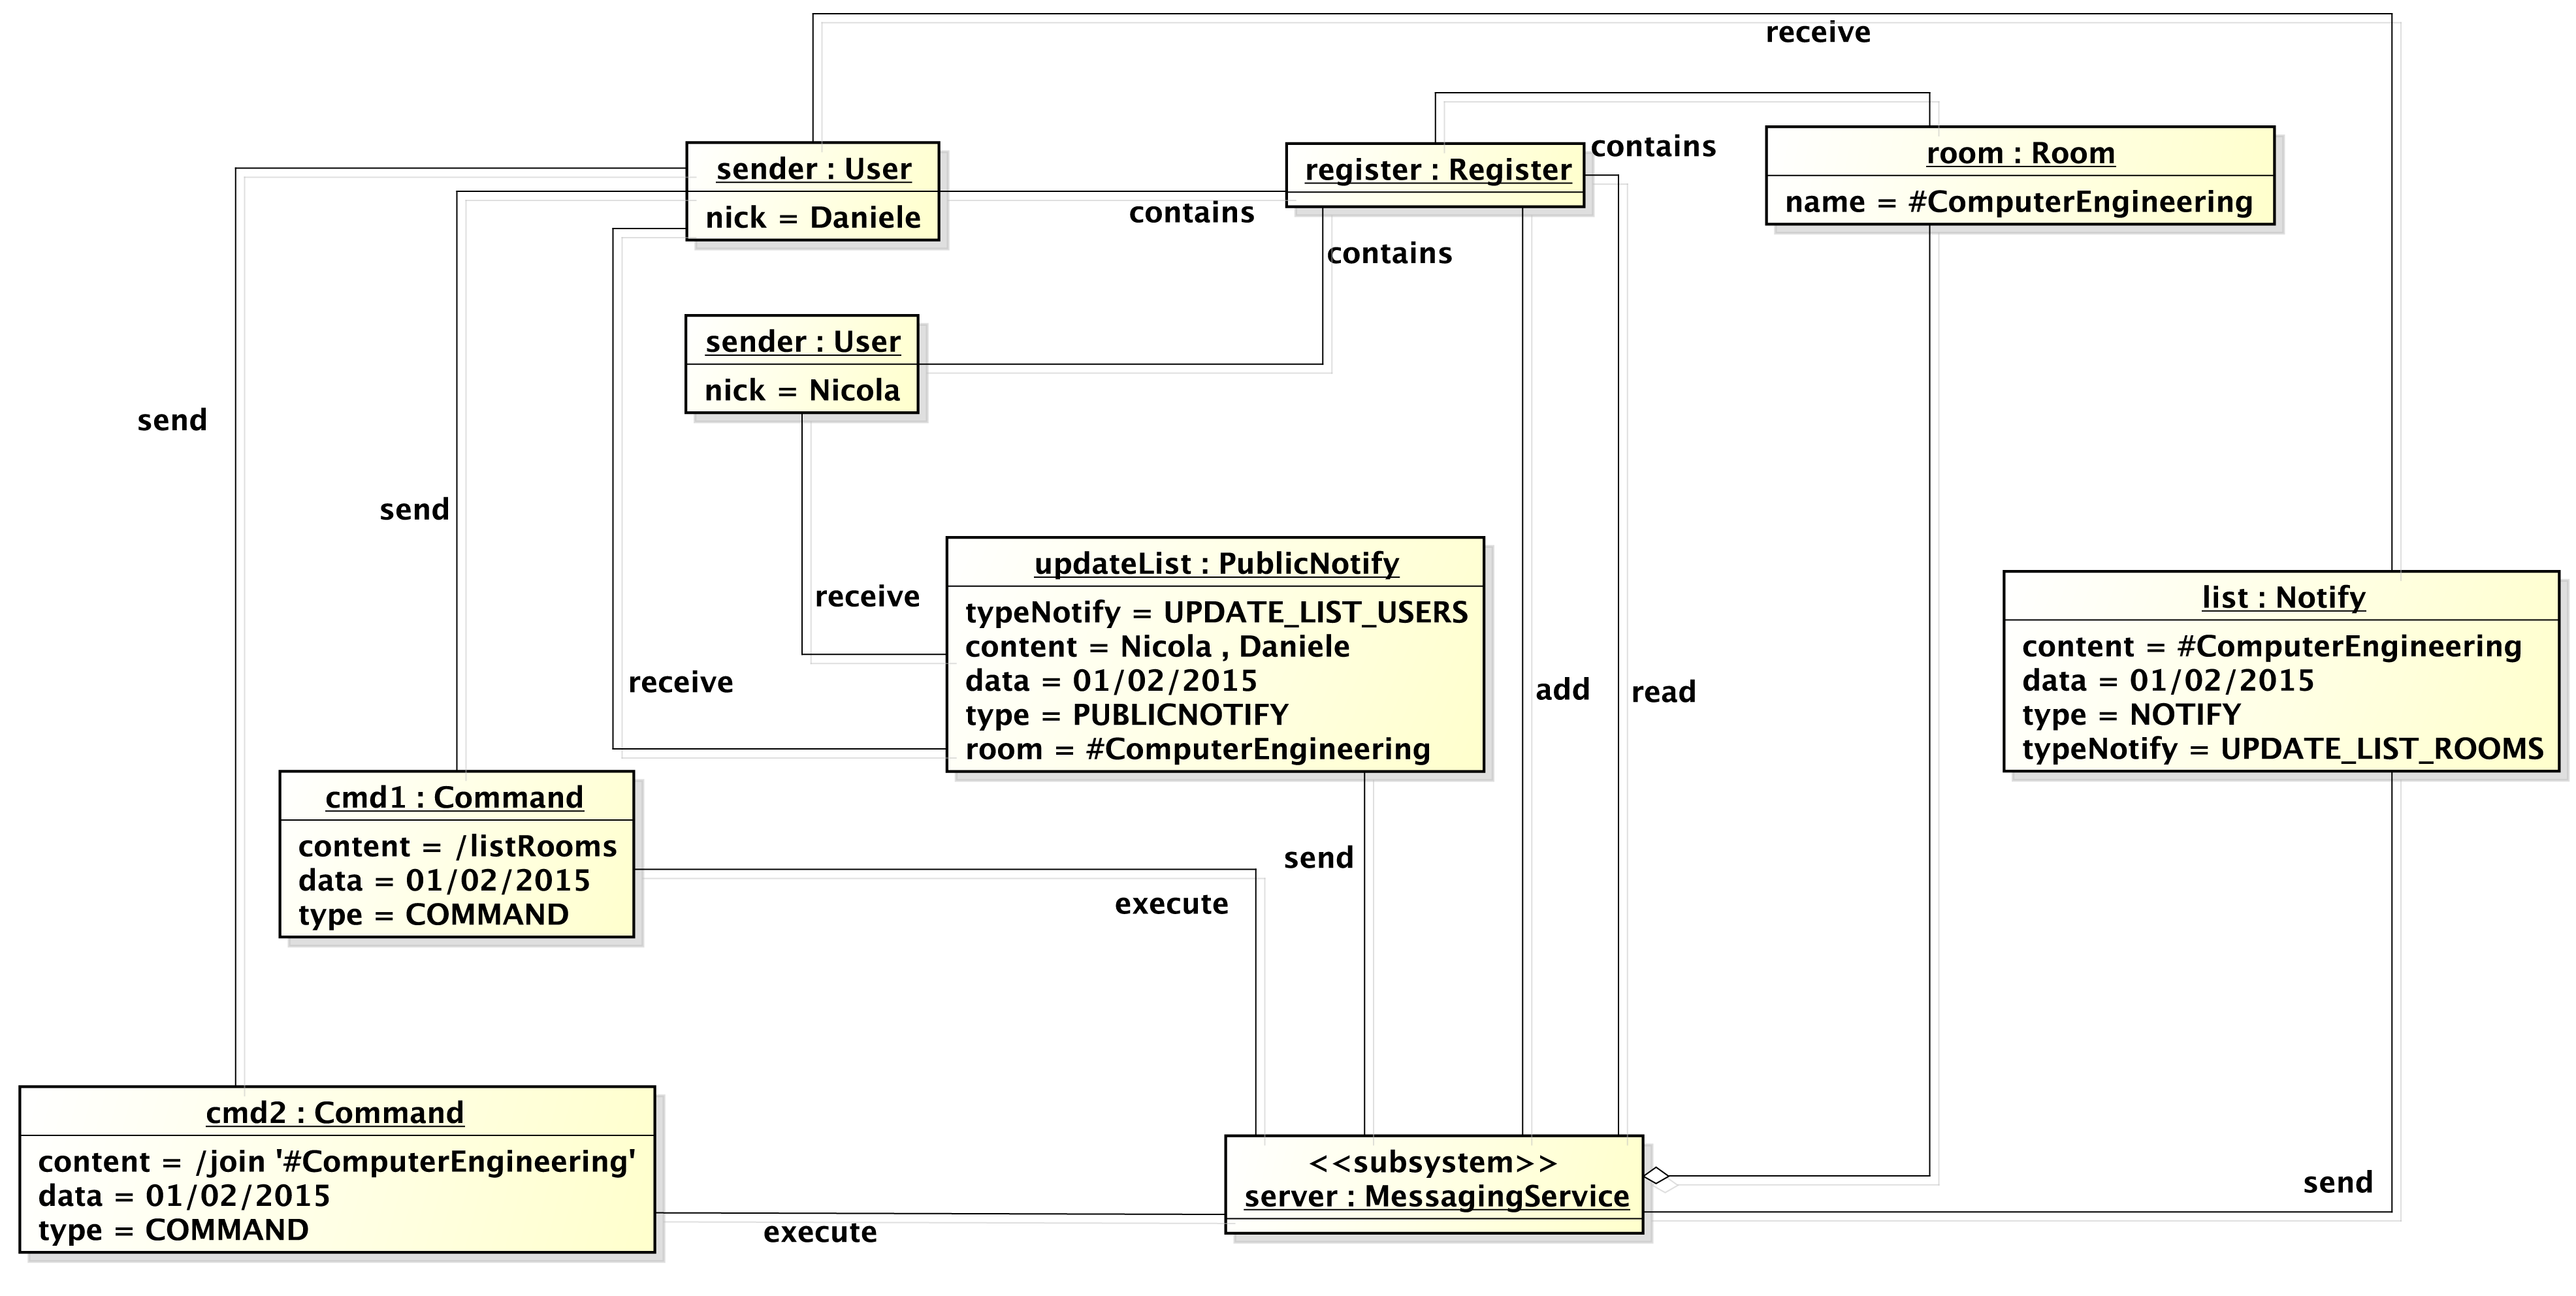
\includegraphics[scale=0.17]{image_astah/Iteration_1_DomainModel/UC2_AccessRoom_OM}{\centering}
     \caption{UC2 - Oggetti di dominio}
     \label{fig_UC2_AR_OM} 
   \end{figure}
\end{frame}

\begin{frame} {Iterazione 1: Analisi - UC2\_AccessRoom}
   \begin{figure}
     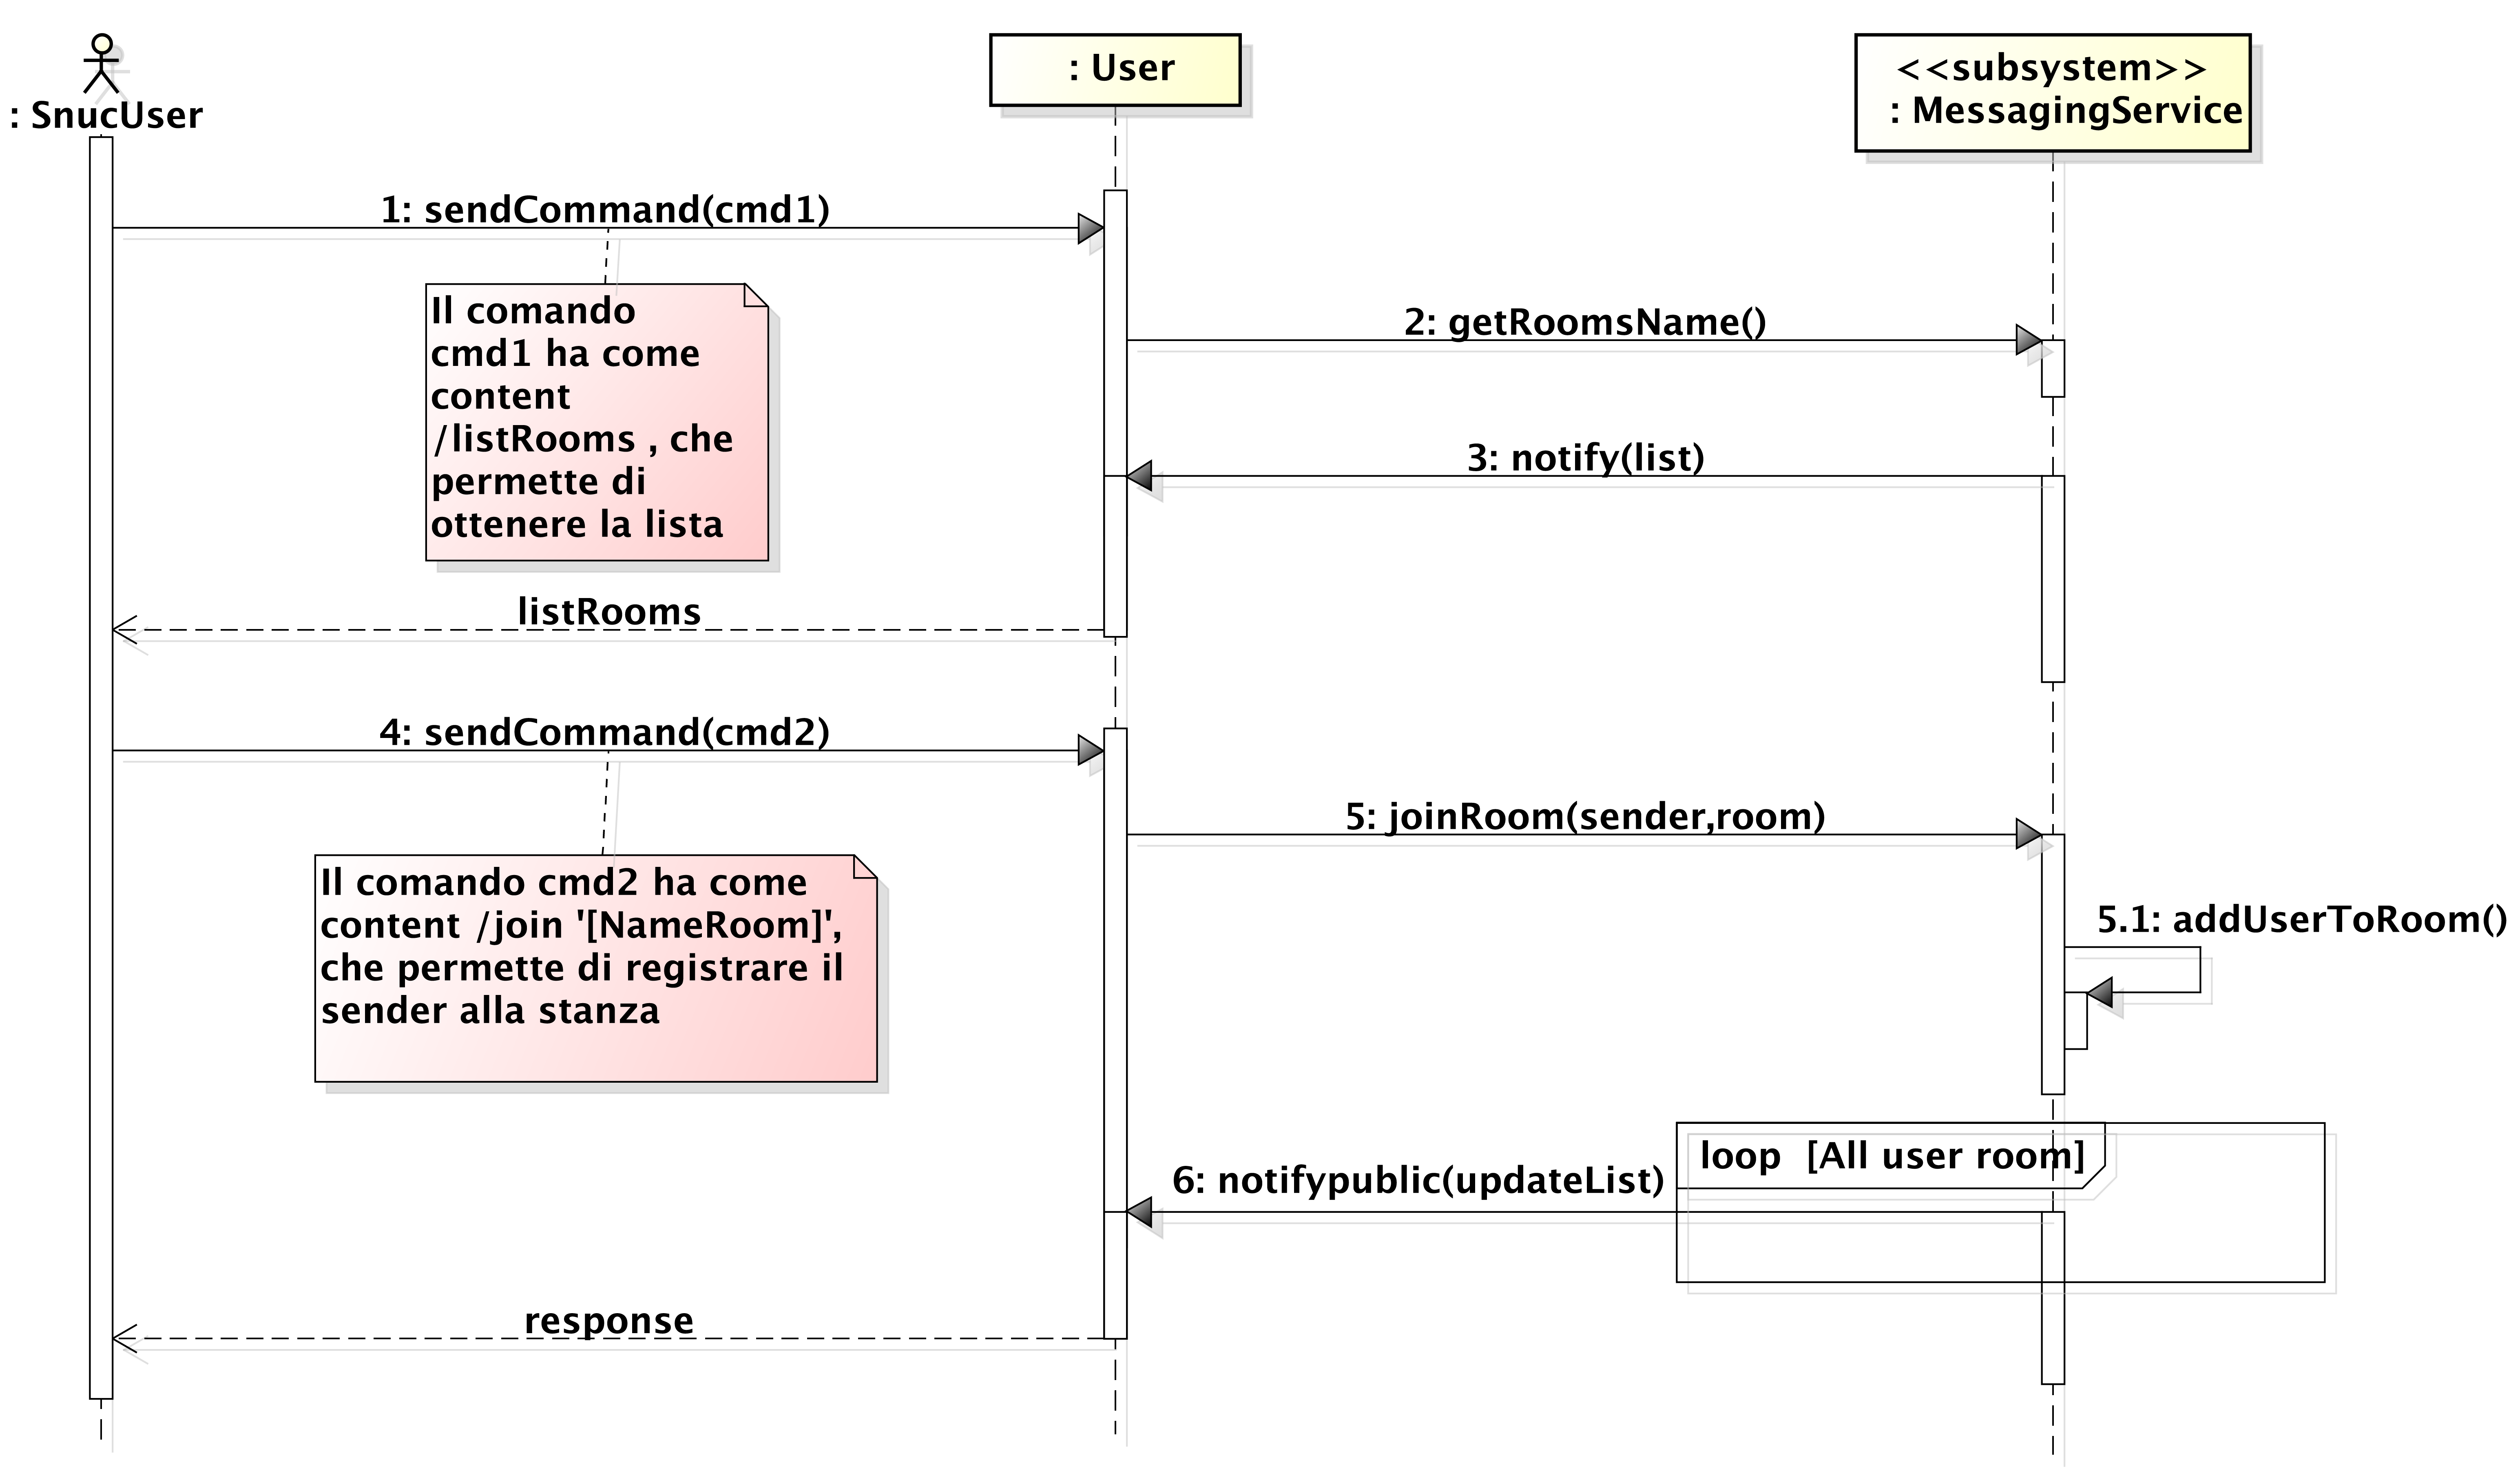
\includegraphics[scale=0.20]{image_astah/Iteration_1_DomainModel/UC2_AccessRoom_SSD.png}{\centering}
     \caption{UC2 - Diagramma di sequenza di dominio}
     \label{fig_UC2_AR_SSD} 
   \end{figure}
\end{frame}

\begin{frame} [allowframebreaks]
 \frametitle{Iterazione 1: Analisi - UC2 contratti CO3/CO4}
  \begin{table}[!htbp]
   \caption {UC2 Contratto CO3 - joinRoom}
    \label{table_CO3}
      \resizebox{\linewidth}{!}{%
       \begin{tabular}{|l|p{10cm}|}\hline
         Operazione & \textit{joinRoom(sender: String, room: String)} \\\hline 
         Riferimenti & Caso d'uso: UC2\_AccessRoom \\\hline
         Pre-condizione & 
         \begin{itemize}
          \item L'utente è connesso al servizio di messaggistica
          \item L'utente ha inserito il comando relativo alla registrazione nella stanza       
         \end{itemize} \\\hline 
         Post-condizione & Il server interpreta il comando ed inserirà l'utente nella lista degli utenti registrati nella stanza  \\\hline
      \end{tabular}}
   \end{table}
  \begin{table}[!htbp]
   \caption {UC2 Contratto CO4 - notifypublic}
    \label{table_CO4}
      \resizebox{\linewidth}{!}{%
       \begin{tabular}{|l|p{10cm}|}\hline
         Operazione & \textit{notifypublic(n: PublicNotify)} \\\hline 
         Riferimenti & Caso d'uso: UC2\_AccessRoom \\\hline
         Pre-condizione & Registrazione utente tra gli utenti della stanza \\\hline 
         Post-condizione & Tutti gli utenti registrati nella stanza ricevono la notifica pubblica relativa all'aggiornamento della lista degli utenti  \\\hline
      \end{tabular}}
   \end{table}


\end{frame}

%ITERAZIONE 1 PROGETTAZIONE 
\subsection{Iterazione 1: Progettazione - Descrizione }
 Da un'analisi del modello di domino sono state realizzate le seguenti classi:   
\begin{frame} [allowframebreaks] {Iterazione 1: Progettazione - Descrizione}
  \begin{itemize}
   \centerline{\textbf{PACKAGE COMMON}}
   \item \textbf{Message}: è una classe astratta che definisce tutti gli attributi di in un generico messaggio che saranno necessari per la corretta gestione.
                 È costituito da un ``content'' (contenuto del messaggio), da una ``date'' (rappresenta la data) e dal ``sender'' (mittente).
   \item \textbf{Command}: è una sottoclasse di Message e permette di identificare che nel contenuto del messaggio avremo un comando.
   \item \textbf{Notify}: è una sottoclasse di Message che permette di identificare le notifiche inviate dal MessagingServer agli User per evidenziare che vi sono 
          stati dei cambiamenti di stato del sistema. Aggiunge un ulteriore attributo per permettere di distitinguere il tipo di notifica.
   \item \textbf{PublicNotify}: è una sottoclasse di Notify. Questo tipo di notifica viene inviata dal MessagingService a tutti gli utenti che sono registrati in una 
         determinata stanza. È stato dunque necessario aggiungere un ulteriore attributo nel quale viene memorizzata la stanza a cui è riferita. Inoltre in quanto 
         l'utente può essere connesso a più stanze contemporaneamente, l'aggiunta di tale attributo ha permesso all'Utente che riceve una PublicNotify di comprendere 
         a quale stanza è riferita.
  \end{itemize} 
 \end{frame}

\begin{frame} [allowframebreaks] {Iterazione 1: Progettazione - Descrizione}
  \begin{itemize}
   \centerline{\textbf{PACKAGE SNUC}}
   \item \textbf{UserView}: rappresenta l'interfaccia utente. Implementa l'interfaccia UserInteraction.
   \item \textbf{UserController}: è il primo oggetto oltre allo strato UI a ricevere e coordinare una operazione di sistema. Fa in modo che l'interfaccia utente non 
         contenga logica applicativa.
   \item \textbf{User}: è l'oggetto dove sono memorizzati tutti i dati relativi all'utente.
   \item \textbf{UserConnection}: questa classe opera lato Client e si occupa dell' instaurazione della connessione con il servizio di messaggistica, dell'invio e 
         della ricezione di oggetti di tipo Message. In base al tipo di Message ricevuto si occupa di andare a richiamare l'opportuno metodo dell'UserController per 
         la gestione di tale messaggio. Poiché dovrà effettuare la continua ricezione di messaggi è stato necessario lanciare un nuovo Thread che resterà in ascolto 
         per ricevere eventuali messaggi da parte del server.
   \item \textbf{SnucMain}: tale classe si occupa della creazione e dell'avvio di tutti gli oggetti necessari al funzionamento dell'applicazione lato Client.
  \end{itemize} 
 \end{frame}
   
\begin{frame} [allowframebreaks] {Iterazione 1: Progettazione - Descrizione}
  \begin{itemize}
   \centerline{\textbf{PACKAGE SNUCSERVER}}
   \item \textbf{MessagingService}: tale classe che rappresenta il servizio di messaggistica ed in cui sono implementate tutte le funzioni necessarie al 
         funzionamento di tale servizio tra cui per esempio la gestione dell'invio delle notifiche agli User, dell'interpretazione dei comandi e del controllo della 
         disponibilità del nickname. Questa classe lancia inoltre un Thread che si occupa di gestire le connessioni da parte degli User.
   \item \textbf{UserConnectionHandler}: una volta che il MessagingService instaura delle connessioni crea degli oggetti di questo tipo e da quel momento in poi la 
         comunicazione di rete con il corrispettivo Client sarà gestita da tale oggetto. Si occupa in particolare della ricezione di oggetti di tipo Message e di 
         richiamare l'opportuna procedura del server per la loro gestione. Il MessagingService instanzia un UserConnectionHandler per ogni User che si connette. 
         Questo oggetto, per rimanere in continuo ascolto di richieste da parte del client, lancia un Thread che effettua tale operazione.
   \item \textbf{Room}: rappresenta la stanza virtuale dove gli user possono registrarsi. Ha quindi un riferimento alla lista degli utenti che sono registrati e 
         implementa tutti i metodi necessari per la sua gestione.
   \item \textbf{CommandParser}: si occupa di analizzare i comandi inviati dagli User. Effettua una controllo sulla sintassi e fornisce dei metodi utili per 
         prelevare il comando e i suoi eventuali parametri. Non si occupa però dell'interpretazione del comando in quanto tale funzione sarà gestita dal 
         MessagingService. 
  \end{itemize} 
\end{frame}

\subsection{Iterazione 1: Progettazione - Class Diagram UC1 e UC2}
\begin{frame} {Iterazione 1: Progettazione - Class Diagram Common UC1 e UC2}
   \begin{figure}
     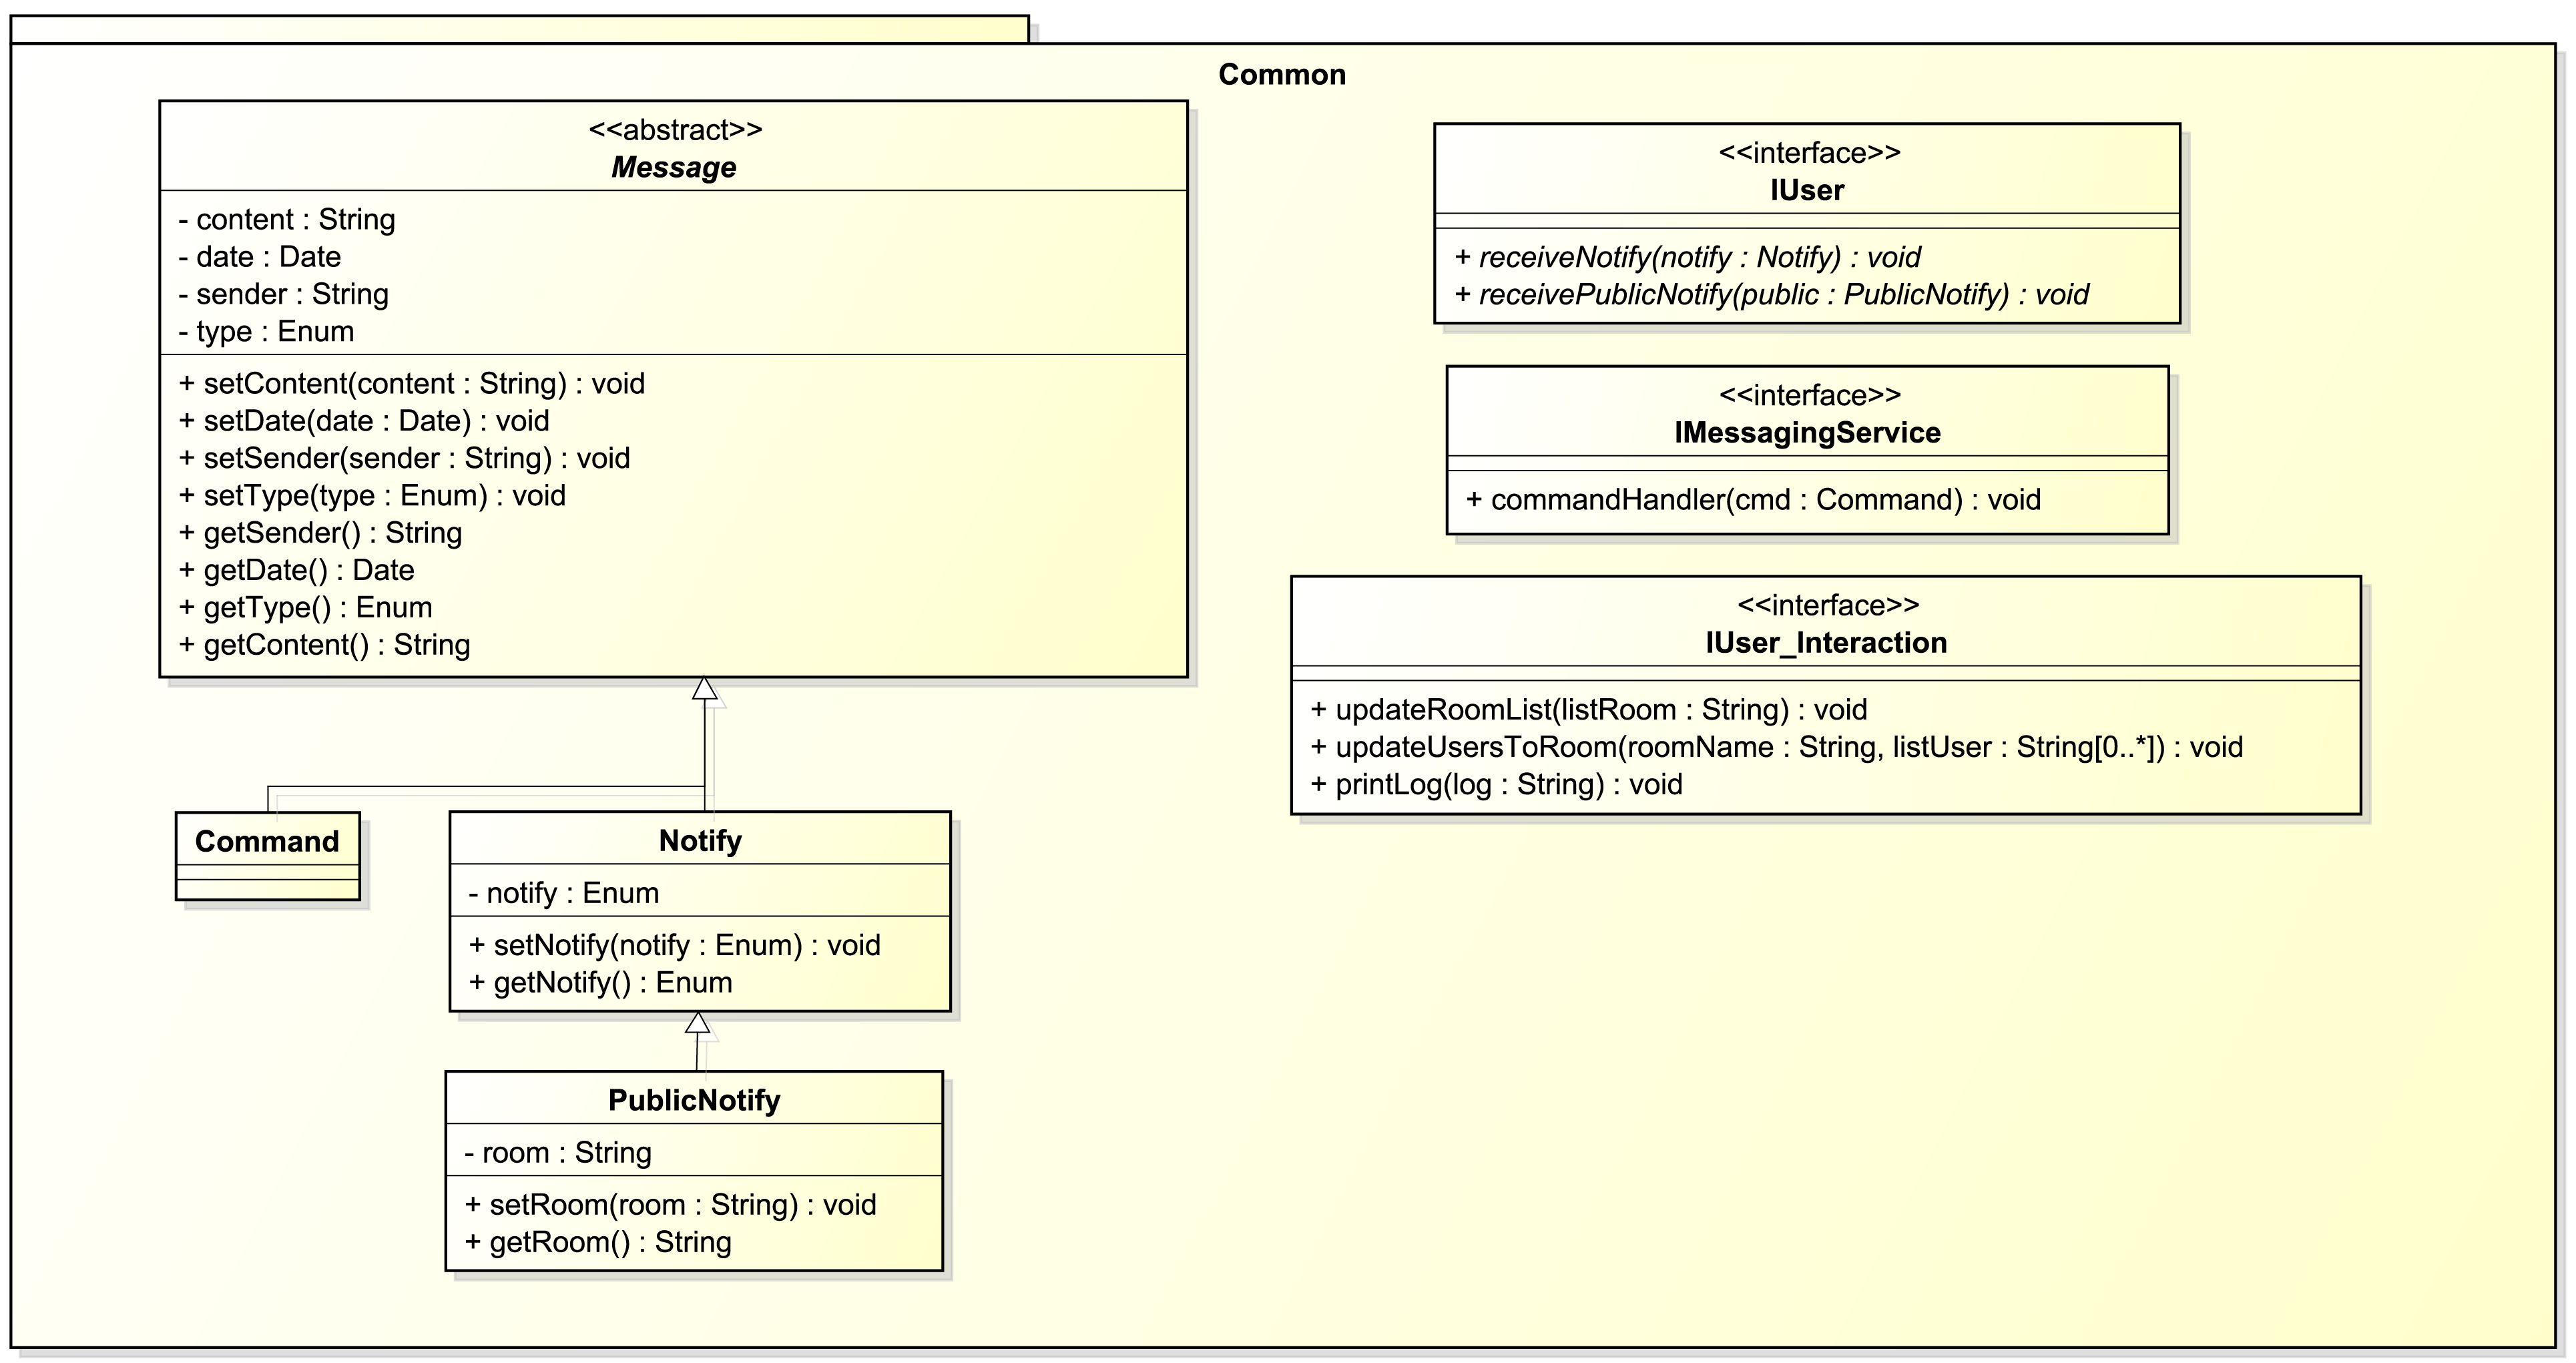
\includegraphics[scale=0.16]{image_astah/Iteration_1_DesignModel/ClassDiagramCommon.png}{\centering}
     \caption{DCD - Diagramma delle Classi: Package Common }
     \label{fig_UC1_UC2_DCD_1} 
   \end{figure}
\end{frame}

\begin{frame} {Iterazione 1: Progettazione - Class Diagram Snuc Server UC1 e UC2}
   \begin{figure}
     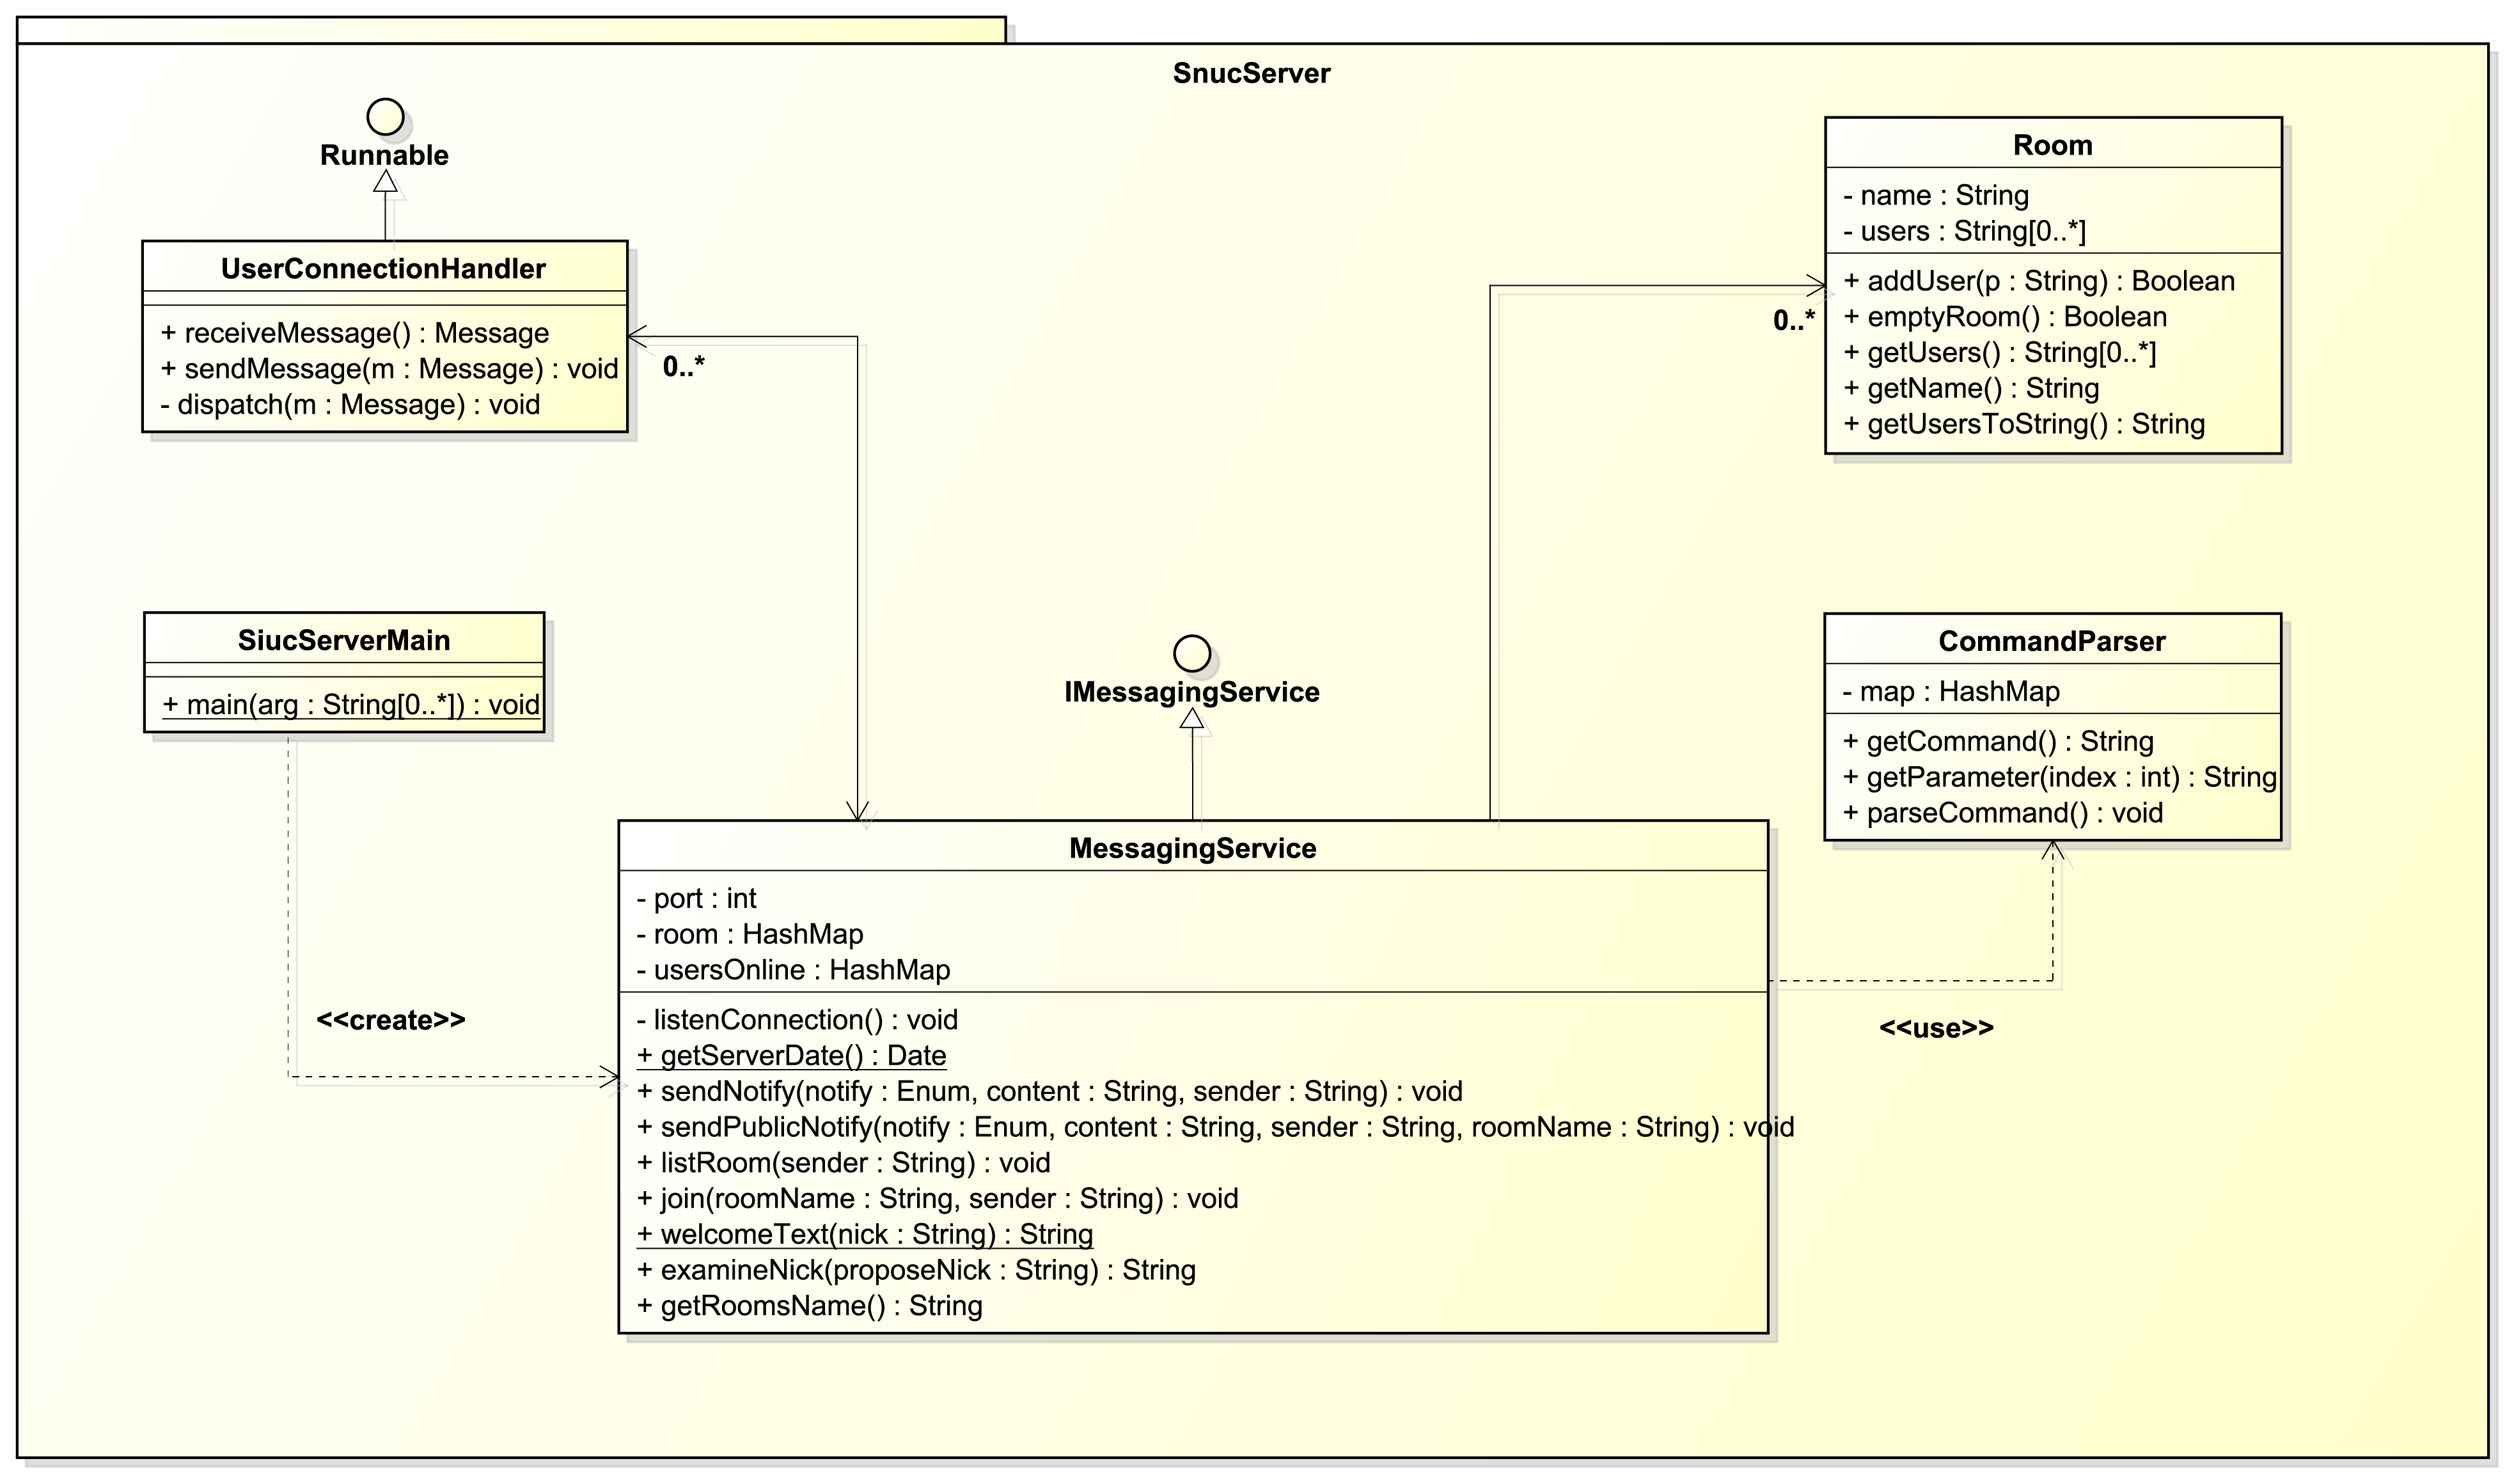
\includegraphics[scale=0.156]{image_astah/Iteration_1_DesignModel/ClassDiagramSnucServer.png}{\centering}
     \caption{DCD - Diagramma delle Classi: Package Snuc Server }
     \label{fig_UC1_UC2_DCD_2} 
   \end{figure}
\end{frame}

\begin{frame} {Iterazione 1: Progettazione - Class Diagram Snuc UC1 e UC2}
   \begin{figure}
     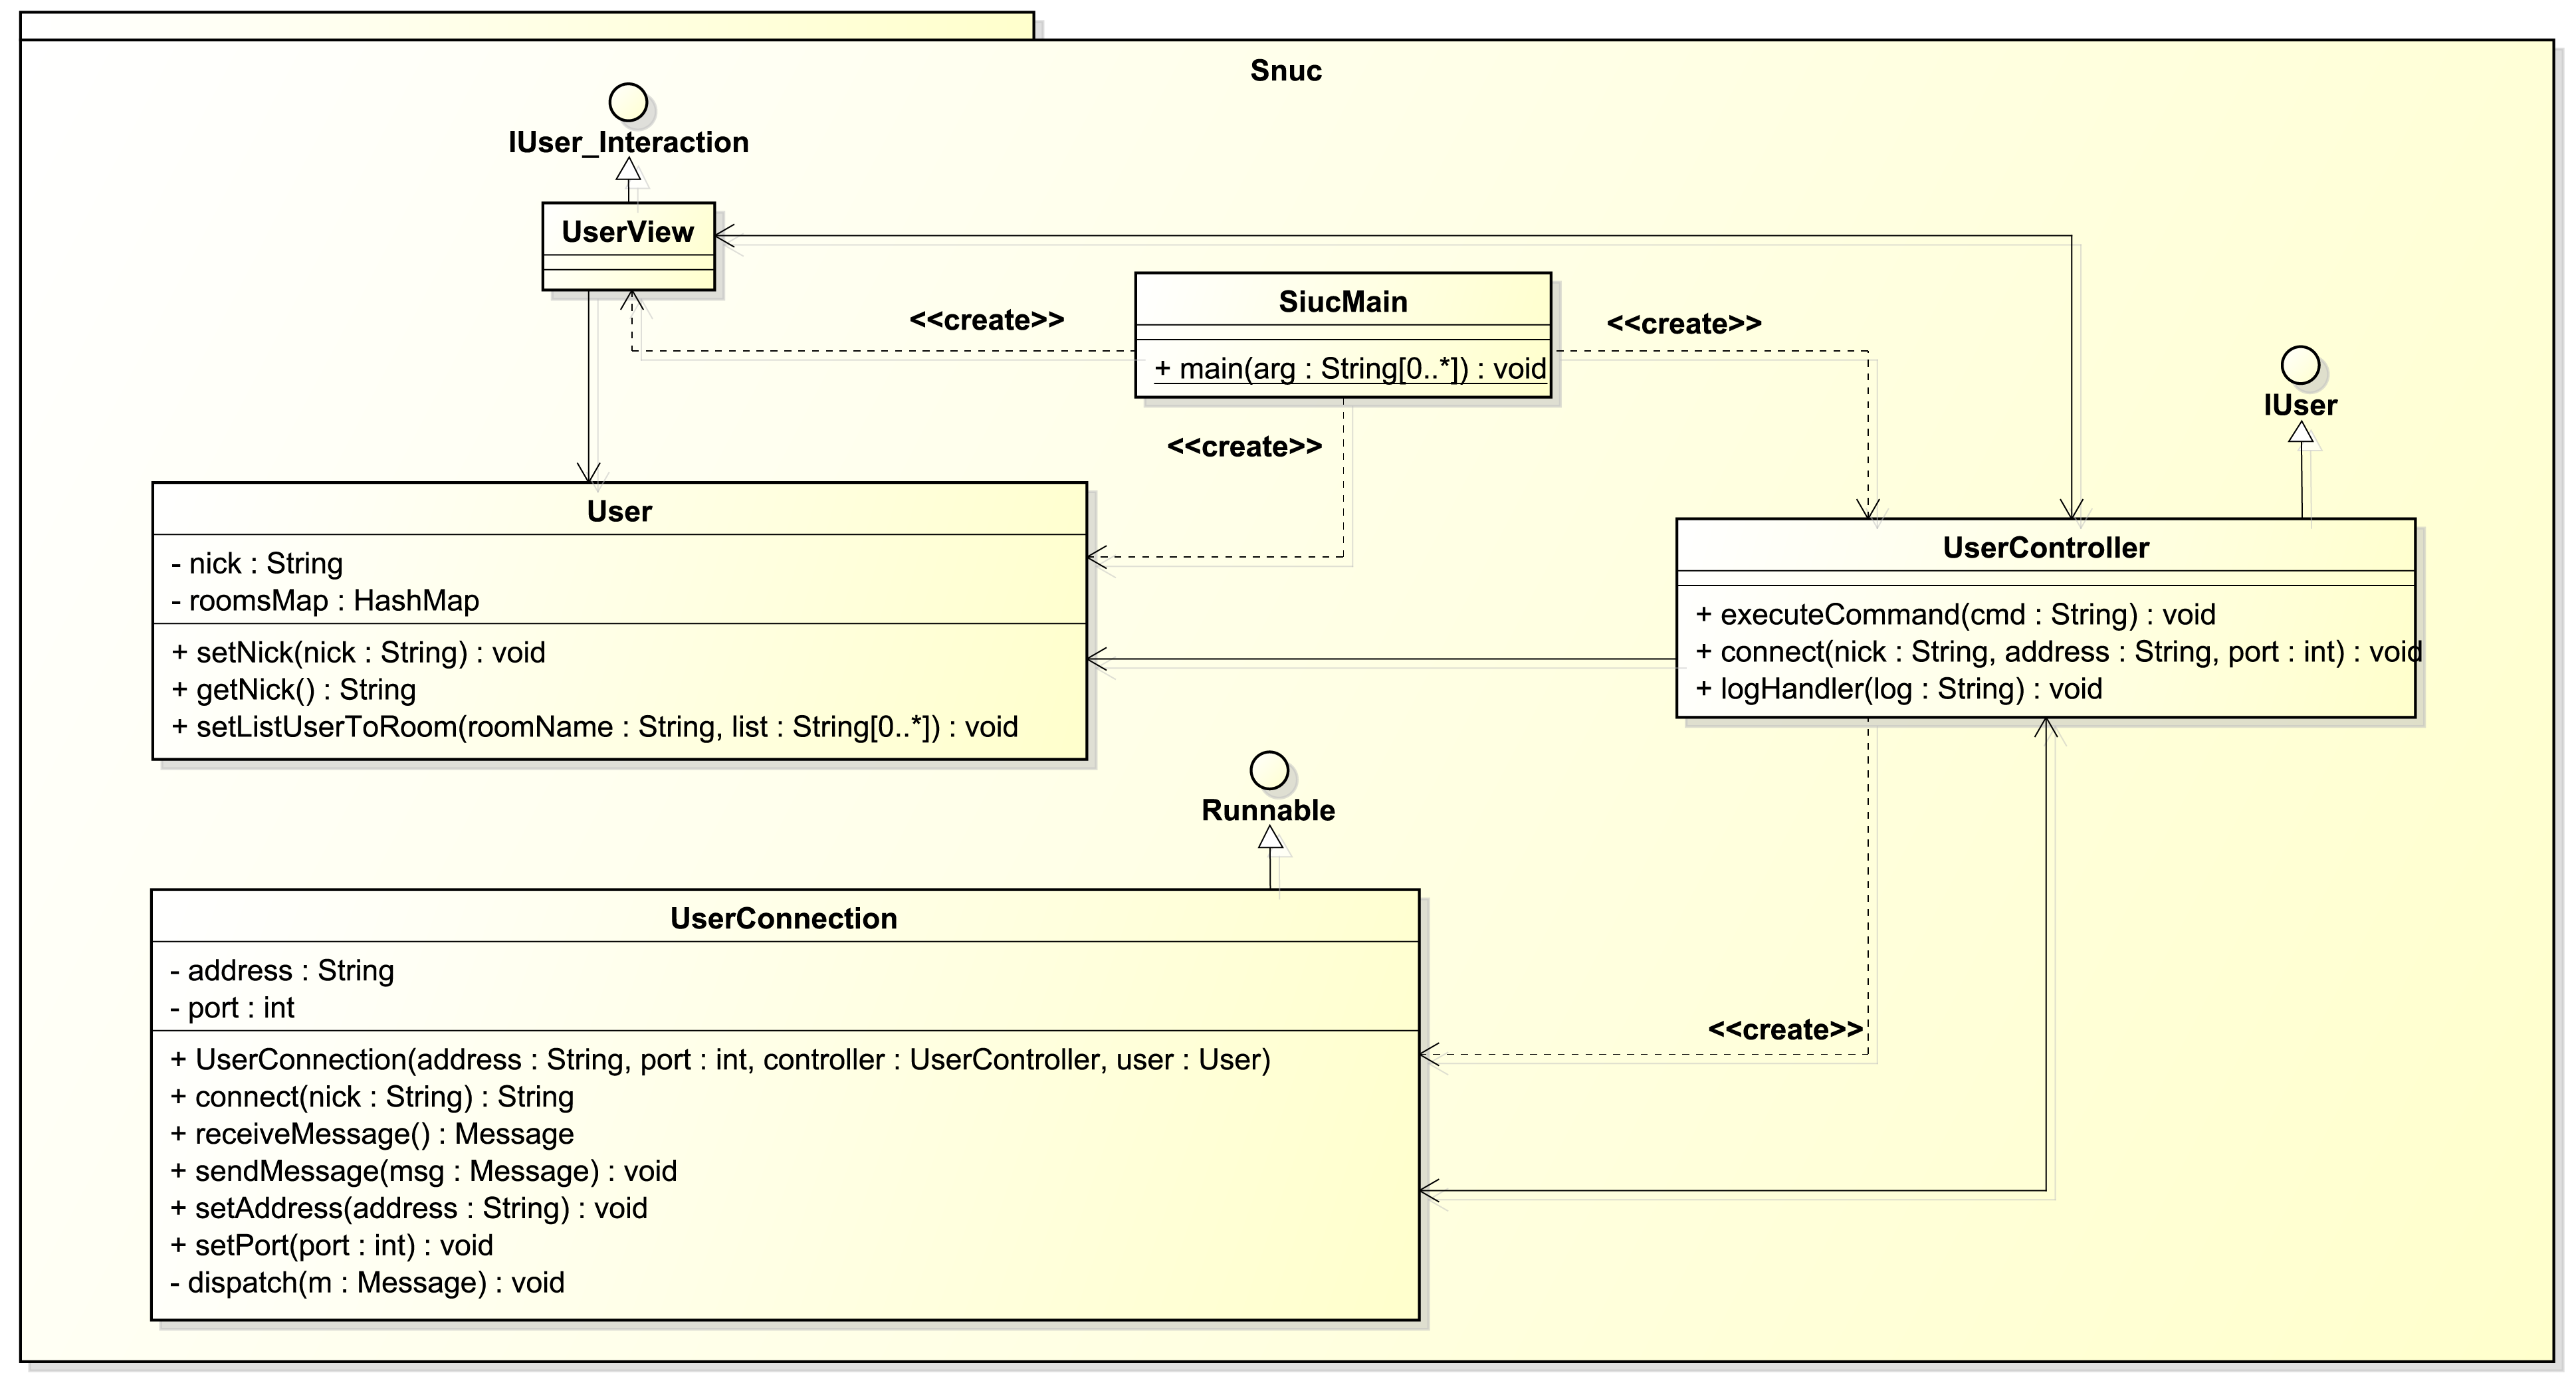
\includegraphics[scale=0.17]{image_astah/Iteration_1_DesignModel/ClassDiagramSnuc.png}{\centering}
     \caption{DCD - Diagramma delle Classi: Package Snuc }
     \label{fig_UC1_UC2_DCD_3} 
   \end{figure}
\end{frame}

\subsection{Iterazione 1: Progettazione - SSD  UC1\_RequestConnection}
\begin{frame} {Iterazione 1: Progettazione, UC1\_RequestConnection}
   \begin{figure}
     %\hypersetup{linkbordercolor={0 0.5 0.1}}
     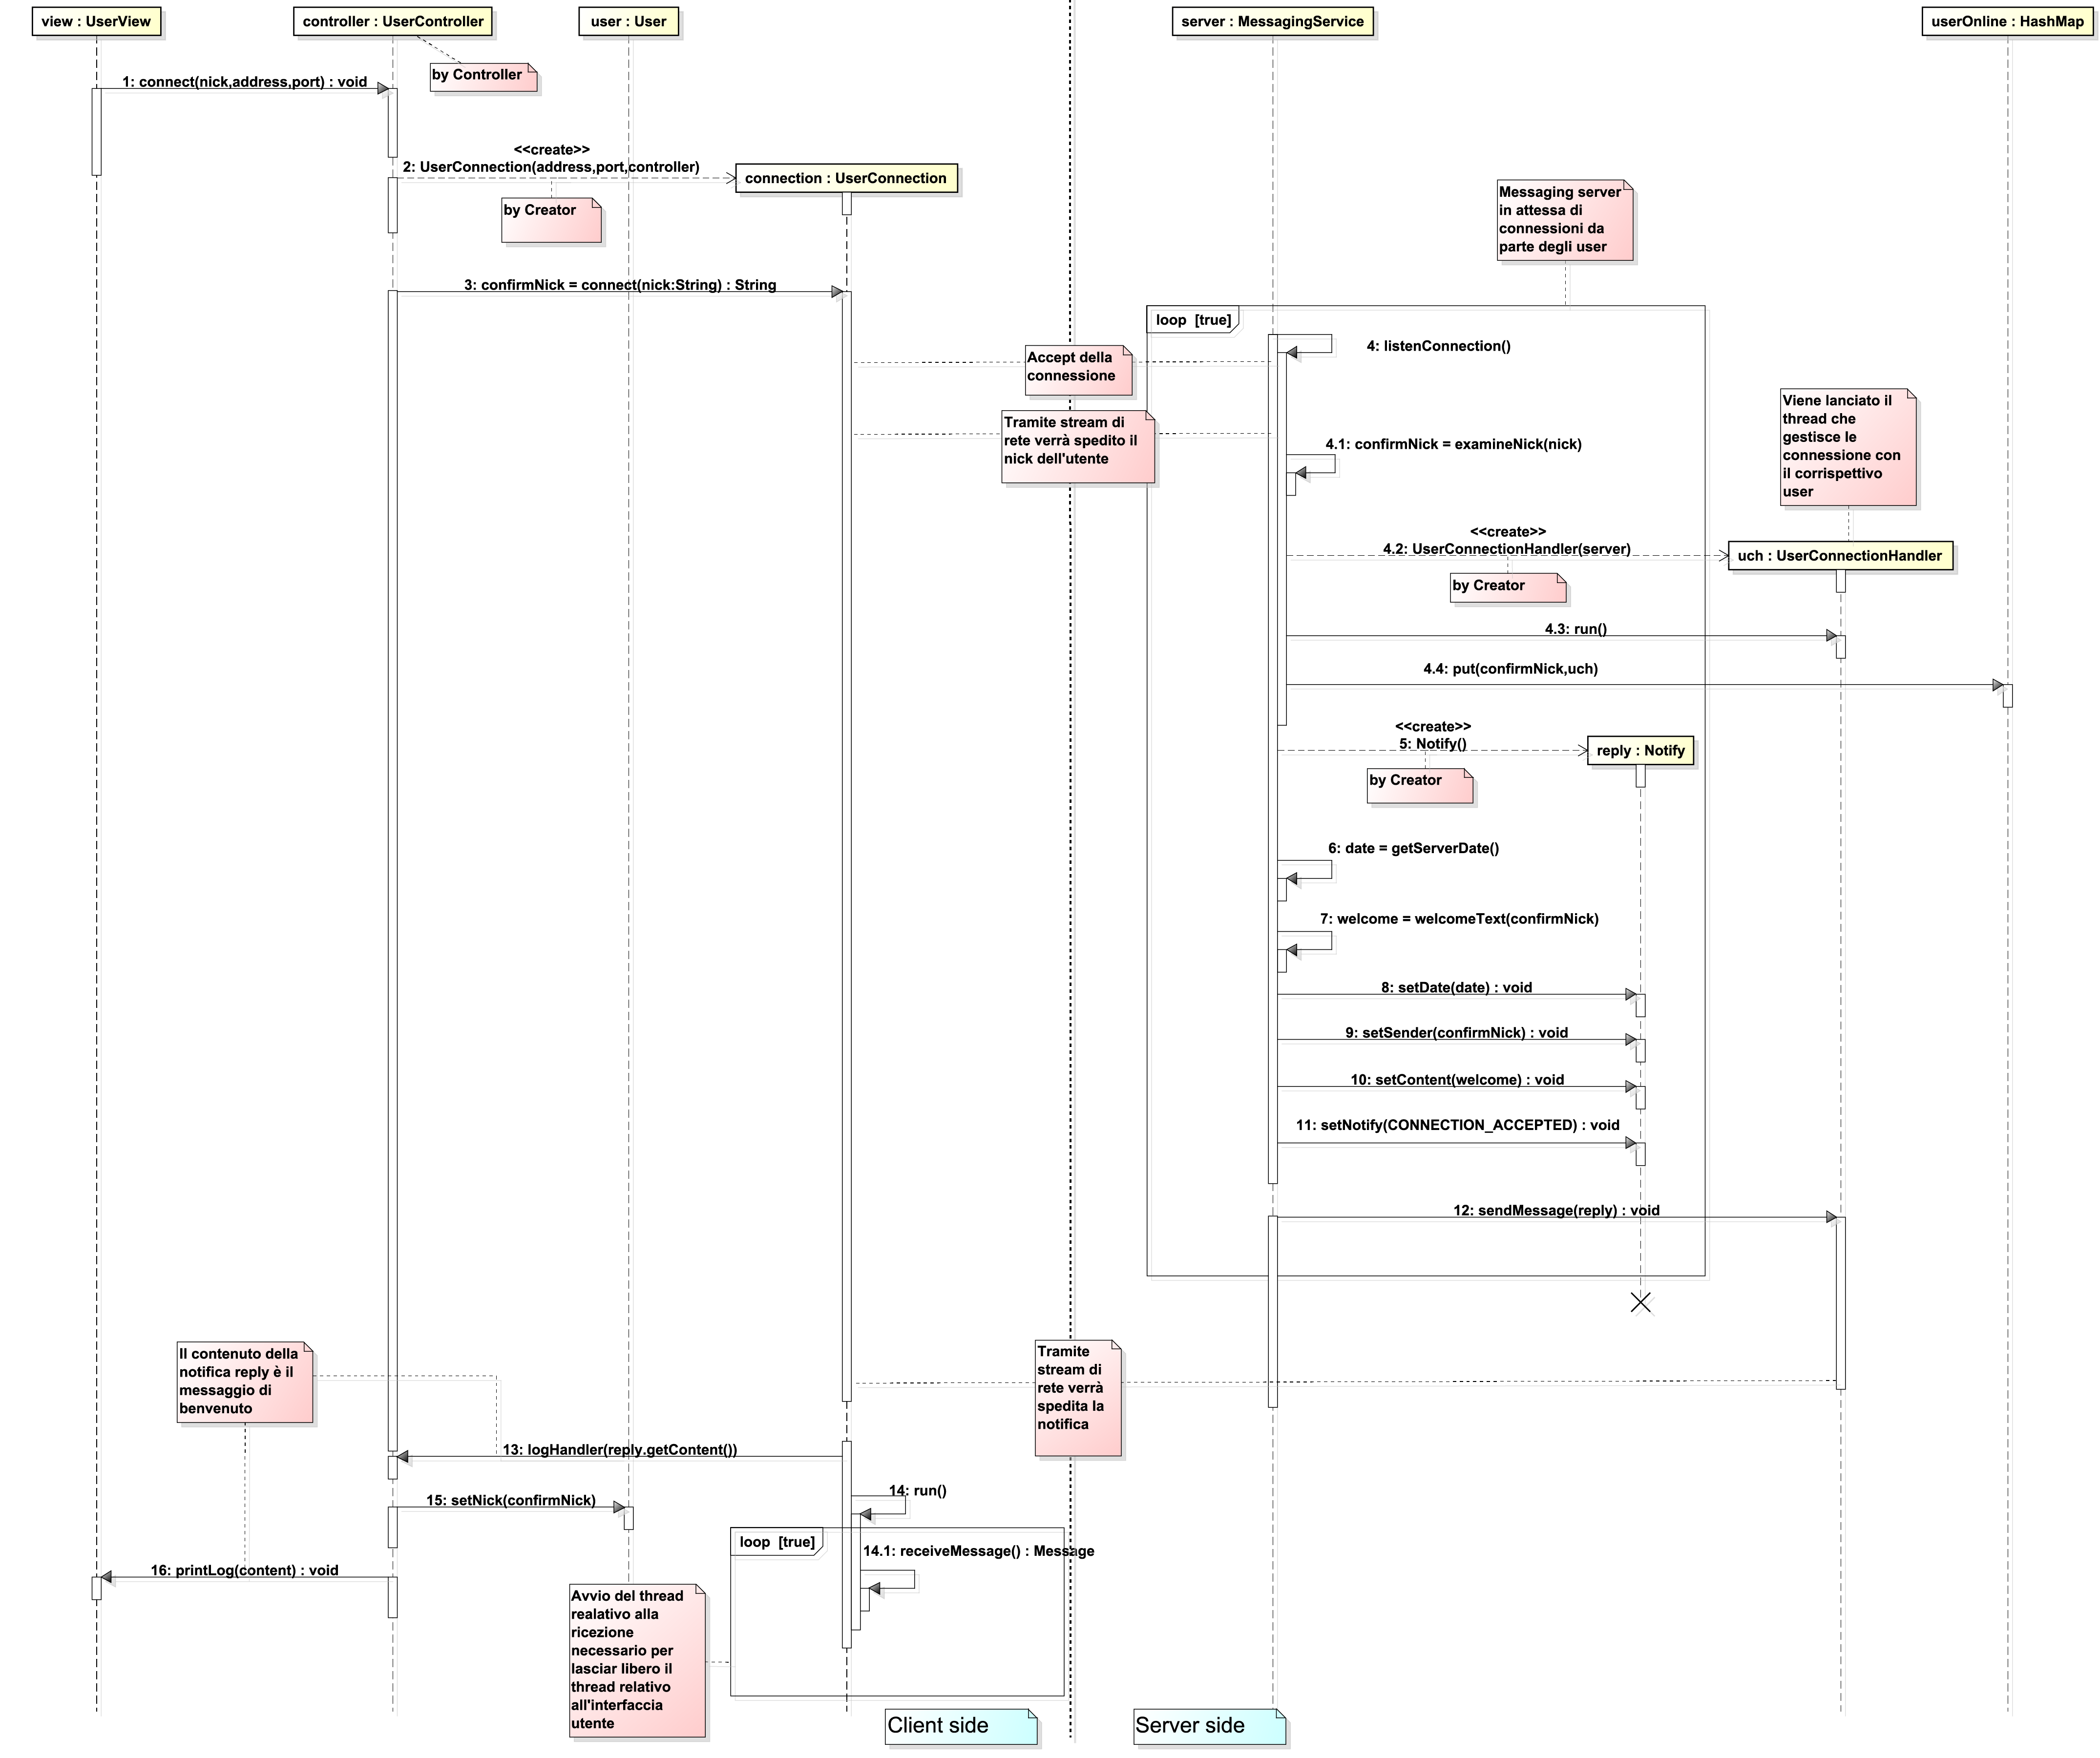
\includegraphics[scale=0.065]{image_astah/Iteration_1_DesignModel/UC1_RequestConnection_SSD_3_4_connect.png}{\centering}
     \caption{SSD - OP1-4: connect(nick), notify(response) del modello dominio (figura \ref{fig_UC1_RC_SSD}) }
     %\framezoom <1><2>[border](0 cm,0.5 cm)(6.8 cm,2.8 cm)% primo quadrante a alto
     %\framezoom <1><4>[border](0 cm,3.5 cm)(6.8 cm,2.8 cm)% secondo quadrante in basso
     \label{fig_UC1_SSD_RC_1_4} 
   \end{figure}
\end{frame}

\subsection{Iterazione 1: Progettazione - SSD UC1\_AccessRoom}
\begin{frame} {Iterazione 1: Progettazione, UC2\_AccessRoom - OP1}
   \begin{figure}
     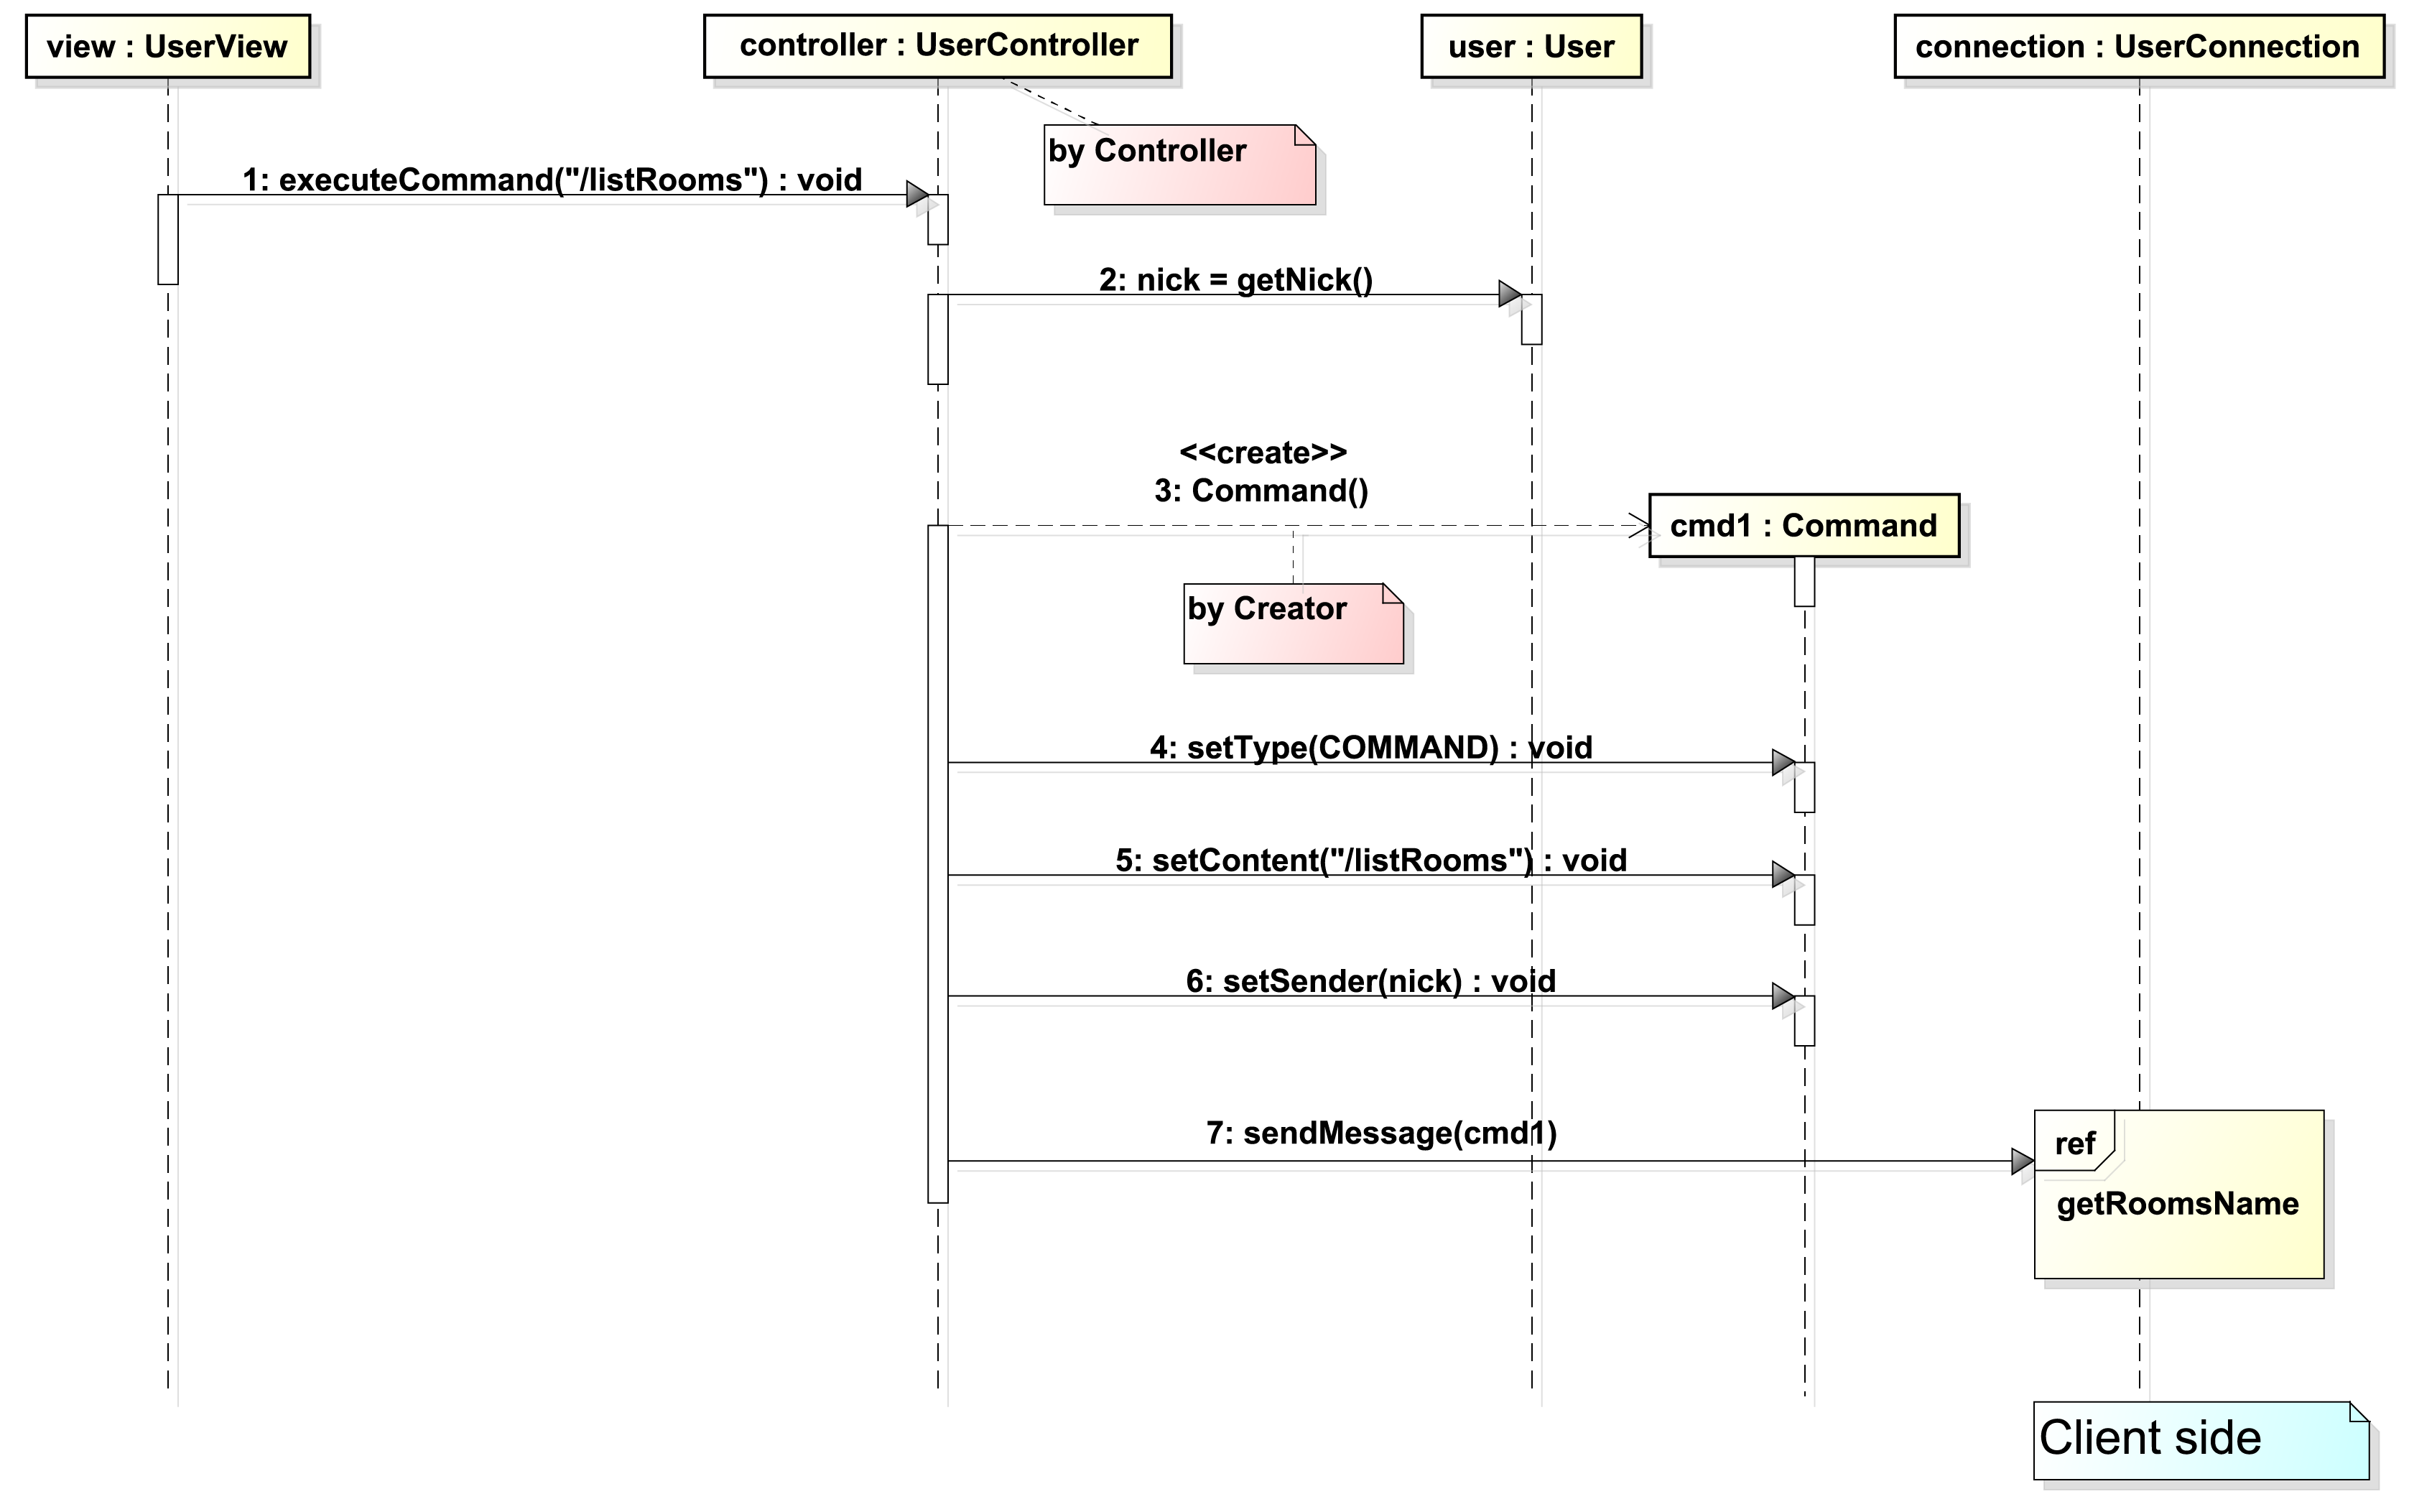
\includegraphics[scale=0.17]{image_astah/Iteration_1_DesignModel/UC2_AccessRoom_SSD_1_sendCommand.png}{\centering}
     \caption{SSD - OP1: sendCommand(cmd1) del modello di dominio (figura \ref{fig_UC2_AR_SSD}) }
     \label{fig_UC2_SSD_AC_1} 
   \end{figure}
\end{frame}

\begin{frame} {Iterazione 1: Progettazione, UC2\_AccessRoom - OP2}
   \begin{figure}
     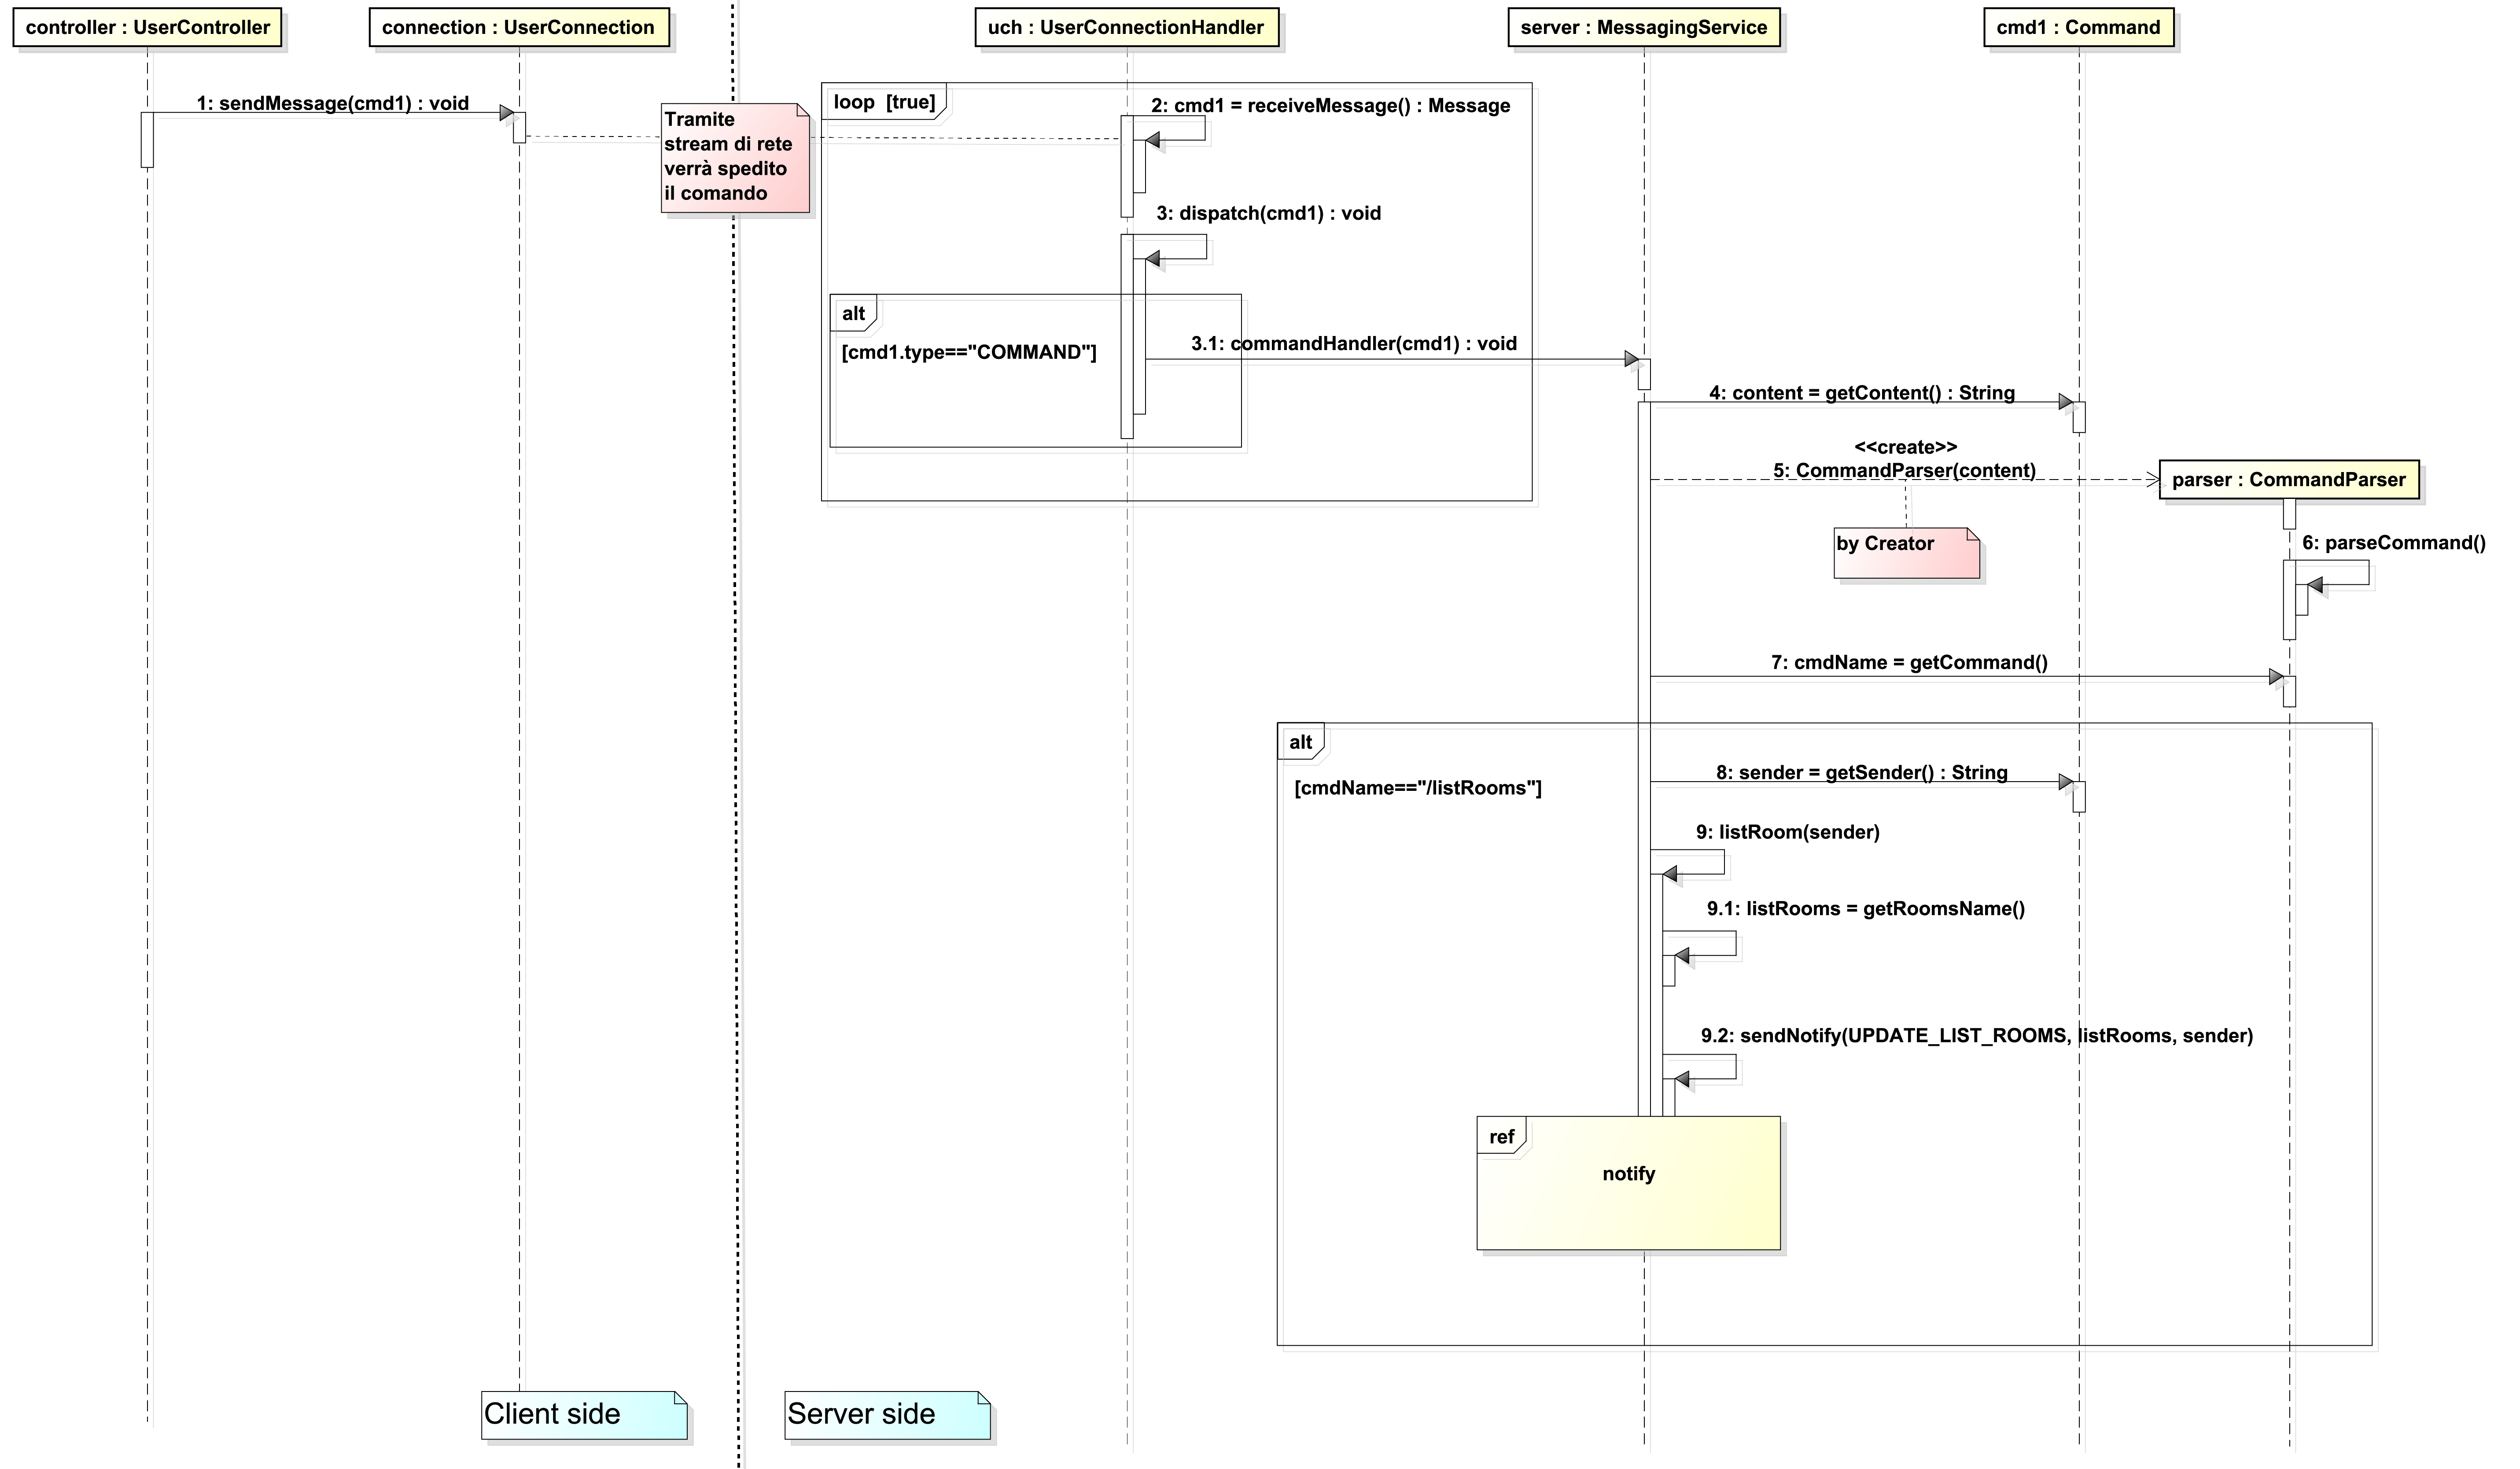
\includegraphics[scale=0.11]{image_astah/Iteration_1_DesignModel/UC2_AccessRoom_SSD_2_getRoomsName.png}{\centering}
     \caption{SSD - OP2: getRoomsName() del modello di dominio (figura \ref{fig_UC2_AR_SSD}) }
     \label{fig_UC2_SSD_AC_2} 
   \end{figure}
\end{frame}

\begin{frame} {Iterazione 1: Progettazione, UC2\_AccessRoom - OP3}
   \begin{figure}
     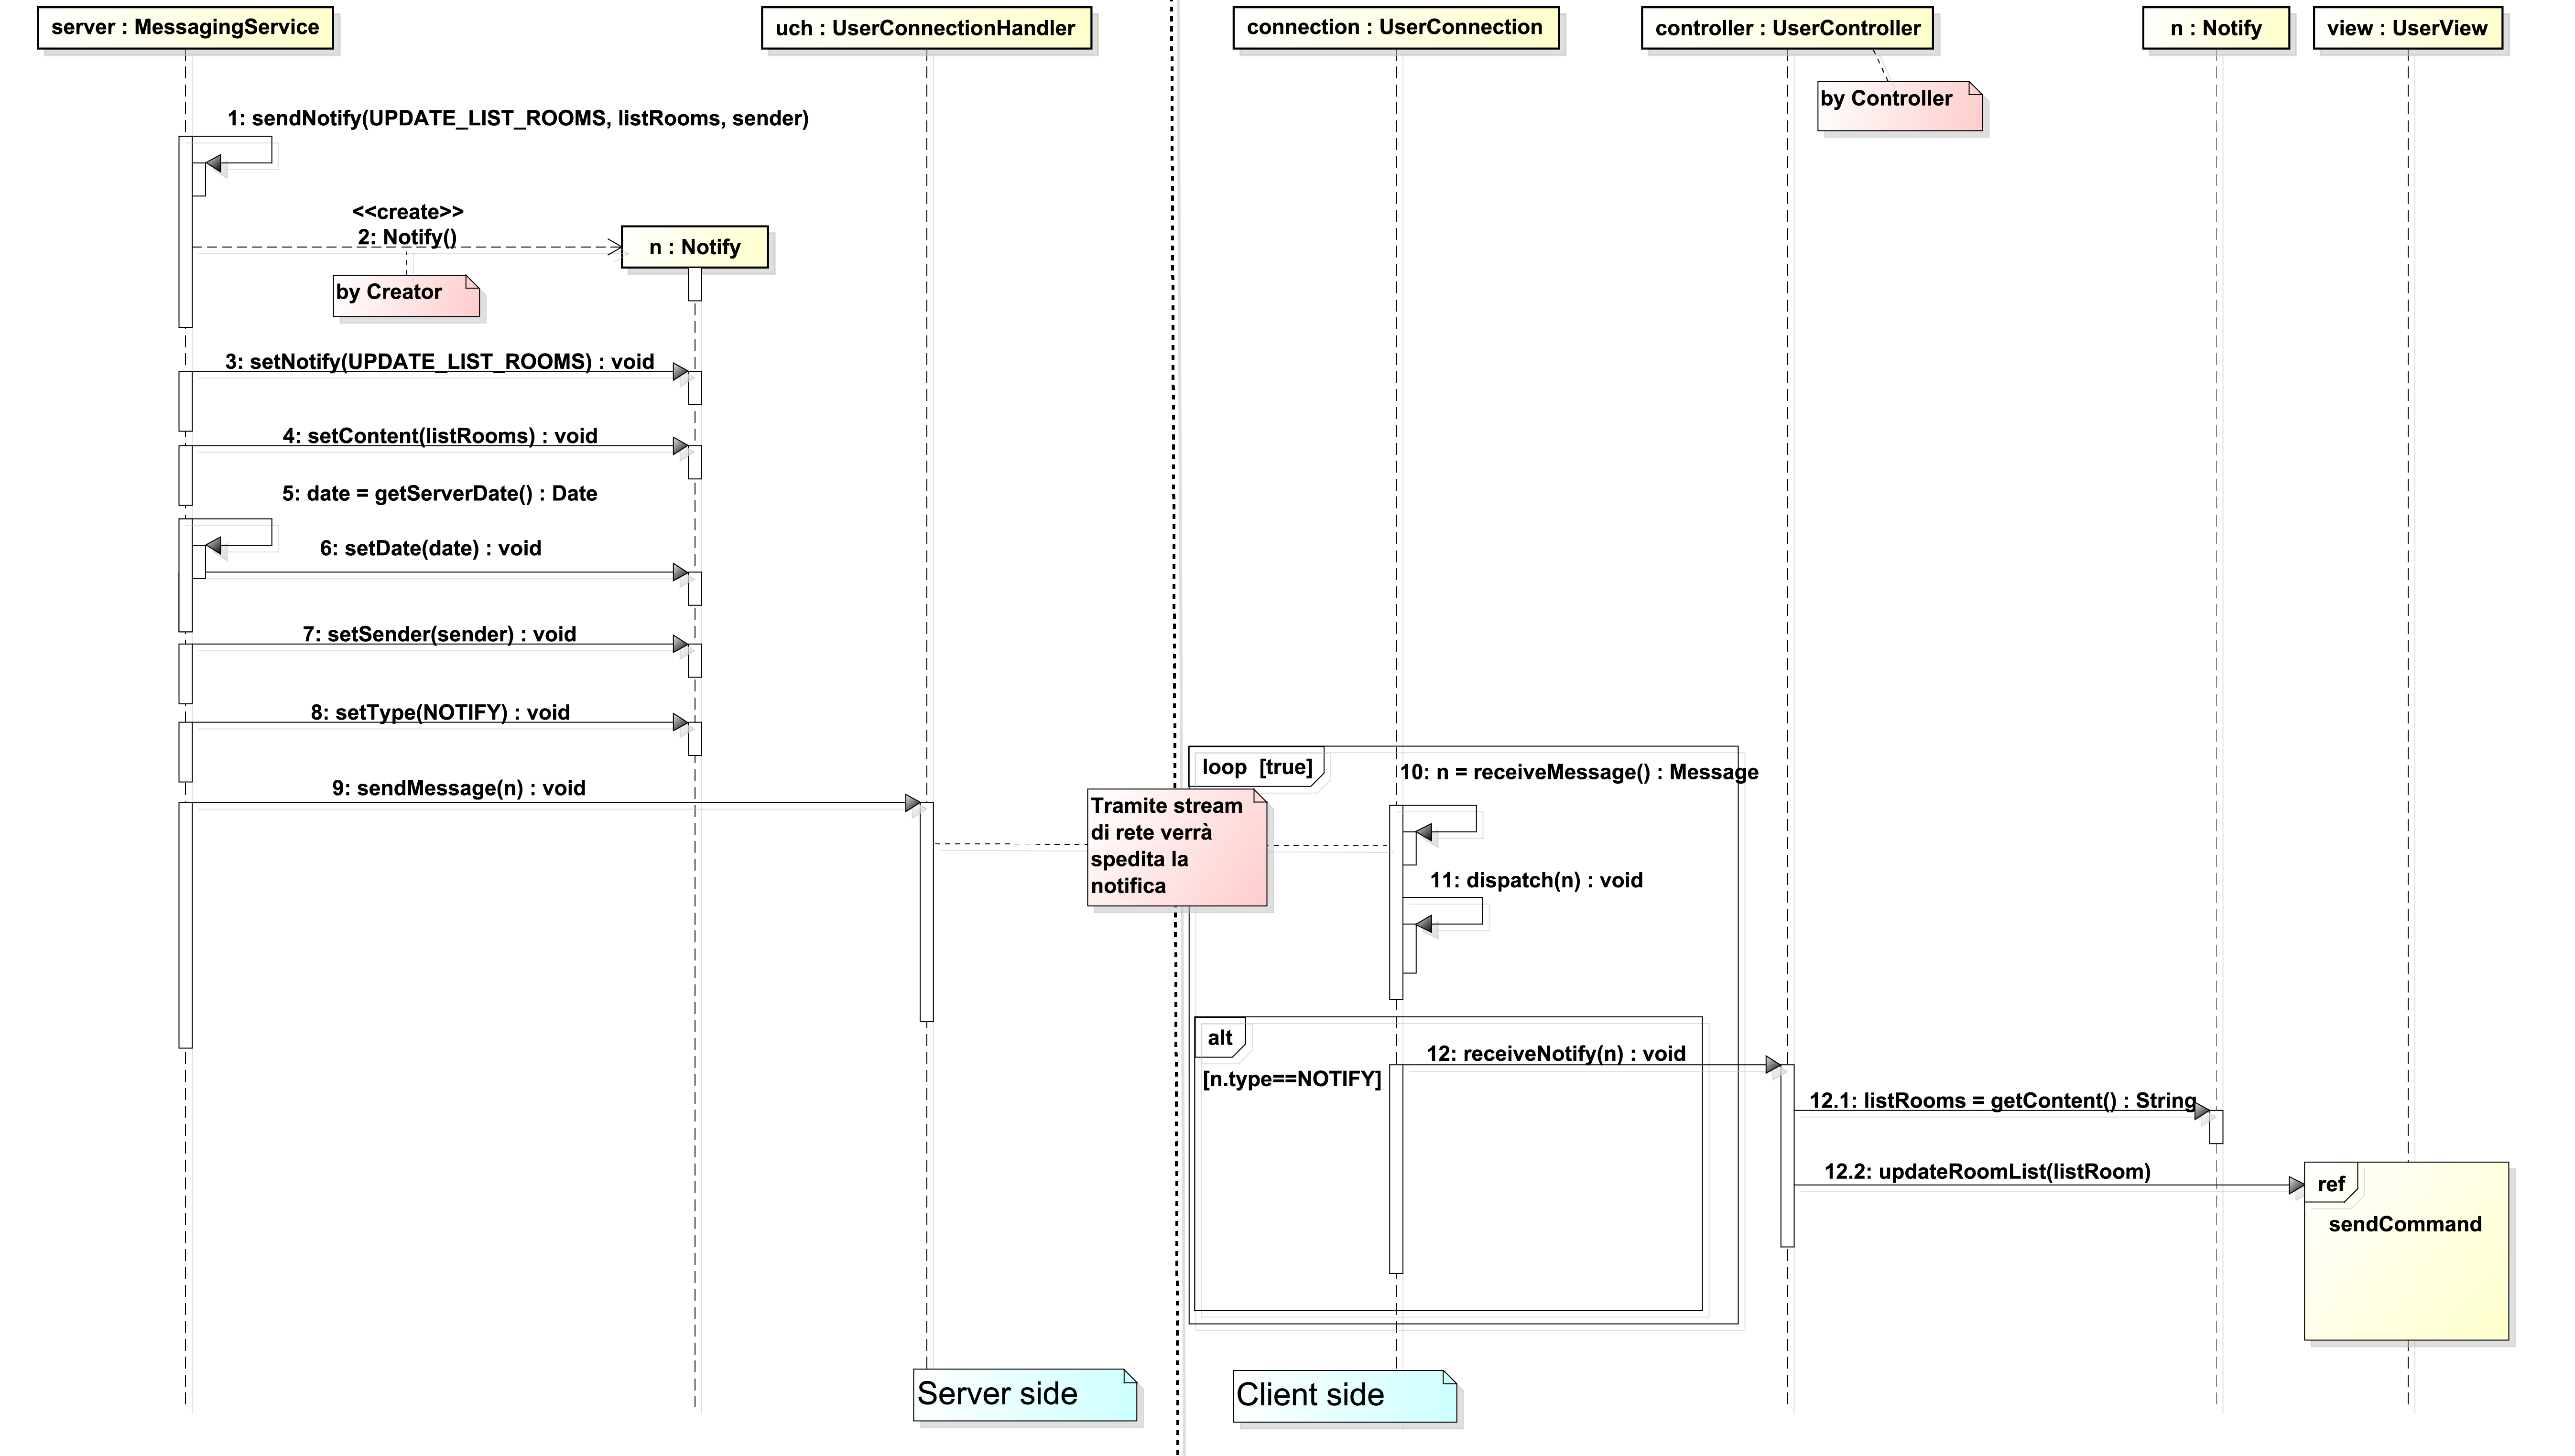
\includegraphics[scale=0.12]{image_astah/Iteration_1_DesignModel/UC2_AccessRoom_SSD_3_notify.png}{\centering}
     \caption{SSD - OP3: notify(list) del modello di dominio (figura \ref{fig_UC2_AR_SSD})}
     \label{fig_UC2_SSD_AC_3} 
   \end{figure}
\end{frame}

\begin{frame} {Iterazione 1: Progettazione, UC2\_AccessRoom - OP4}
   \begin{figure}
     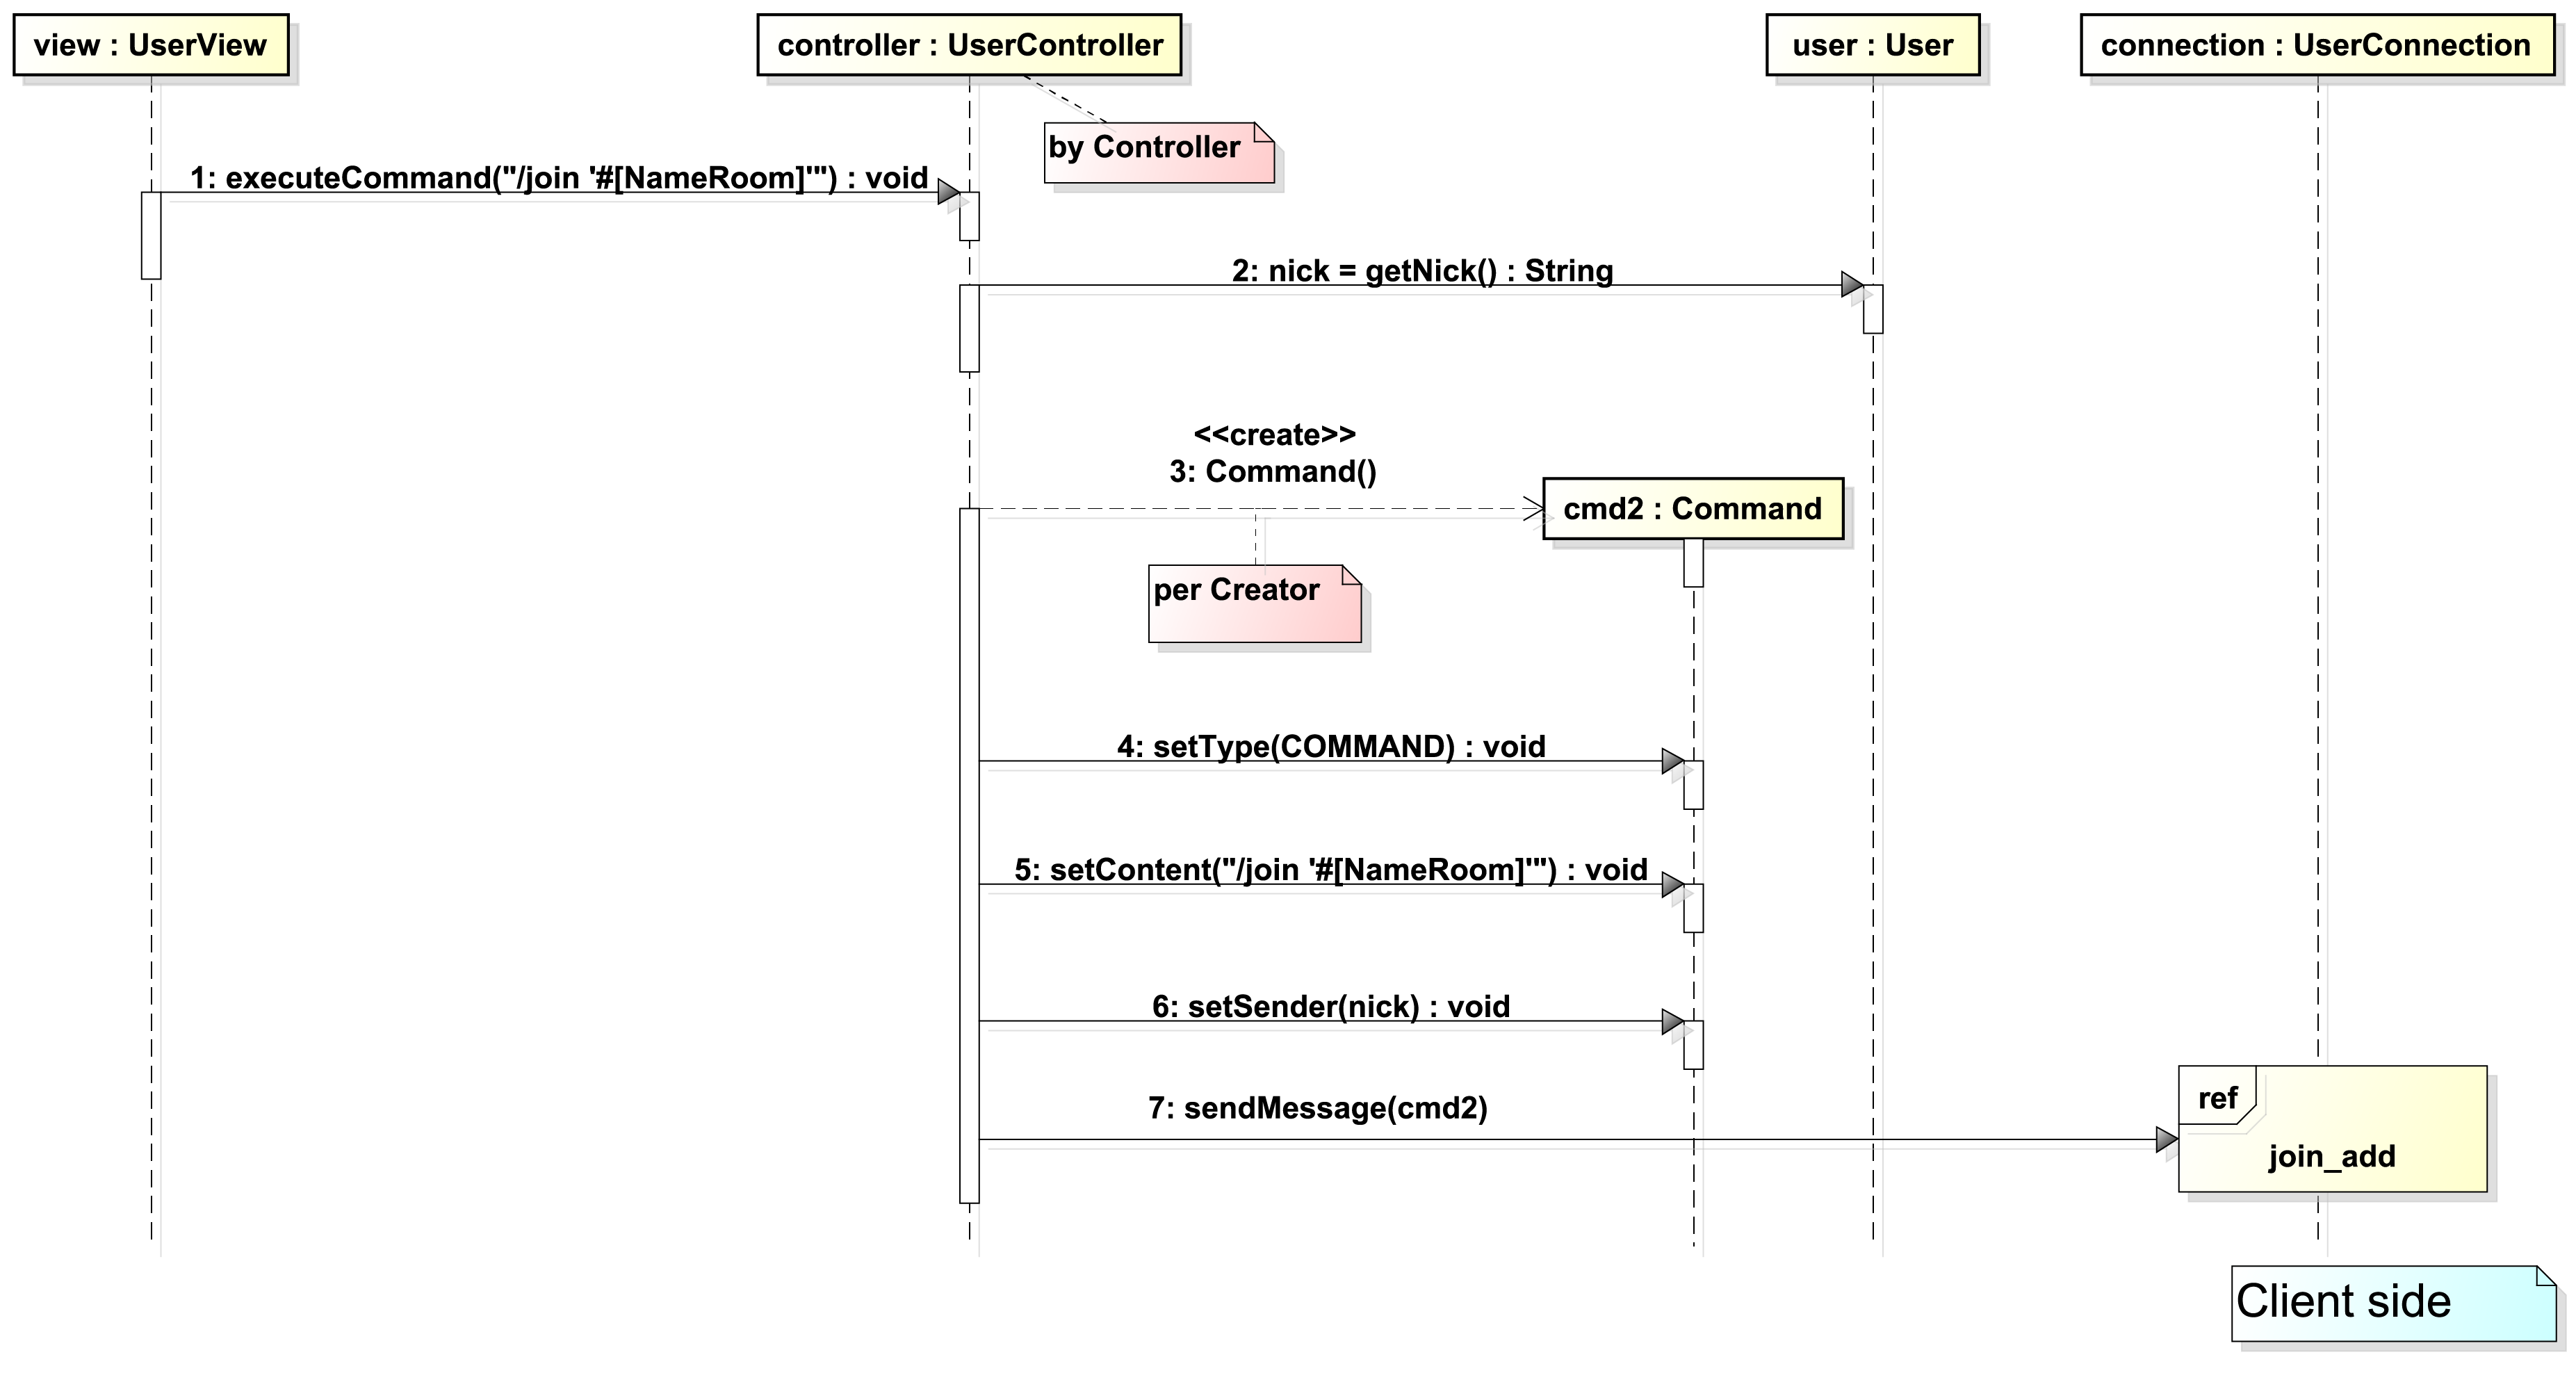
\includegraphics[scale=0.18]{image_astah/Iteration_1_DesignModel/UC2_AccessRoom_SSD_4_sendCommand.png}{\centering}
     \caption{SSD - OP4: sendCommand(cmd2) del modello di dominio (figura \ref{fig_UC2_AR_SSD}) }
     \label{fig_UC2_SSD_AC_4} 
   \end{figure}
\end{frame}

\begin{frame} {Iterazione 1: Progettazione, UC2\_AccessRoom - OP5}
   \begin{figure}
     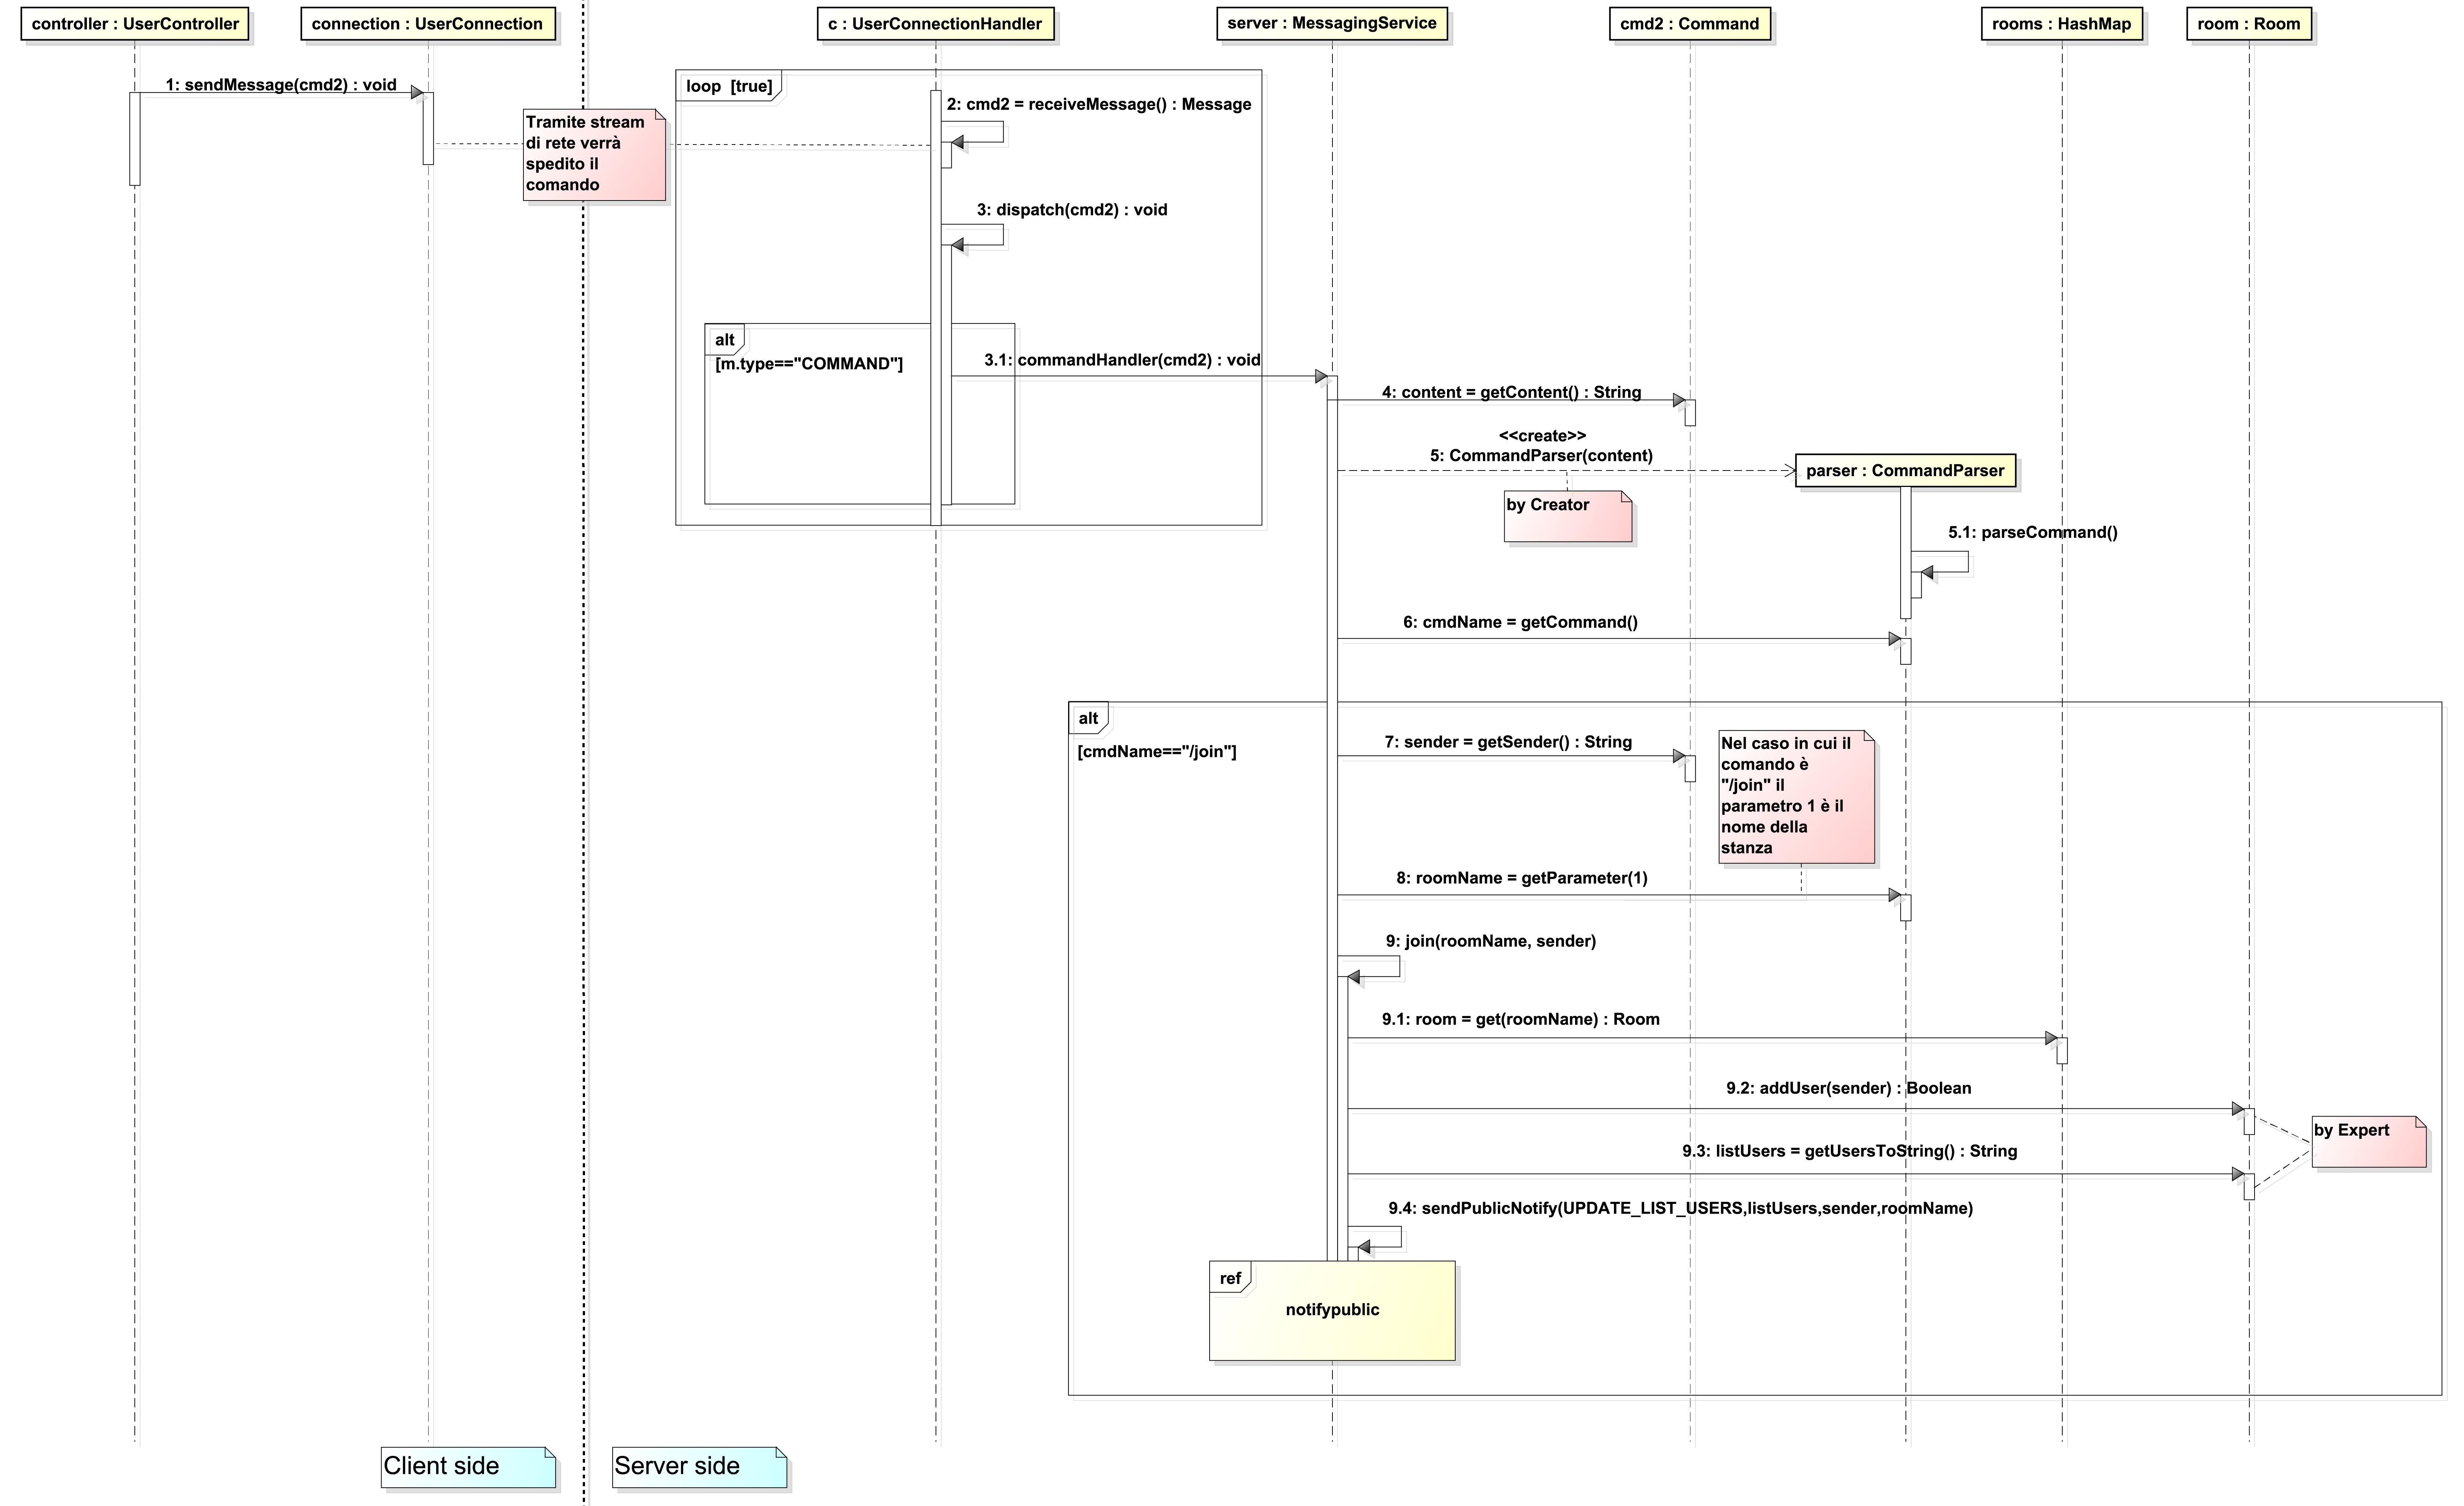
\includegraphics[scale=0.09]{image_astah/Iteration_1_DesignModel/UC2_AccessRoom_SSD_5_join_add.png}{\centering}
     \caption{SSD - OP5: joinRoom(sender,room), addUserToRoom() del modello di dominio (figura \ref{fig_UC2_AR_SSD}) }
     \label{fig_UC2_SSD_AC_5} 
   \end{figure}
\end{frame}

\begin{frame} {Iterazione 1: Progettazione, UC2\_AccessRoom - OP6}
   \begin{figure}
     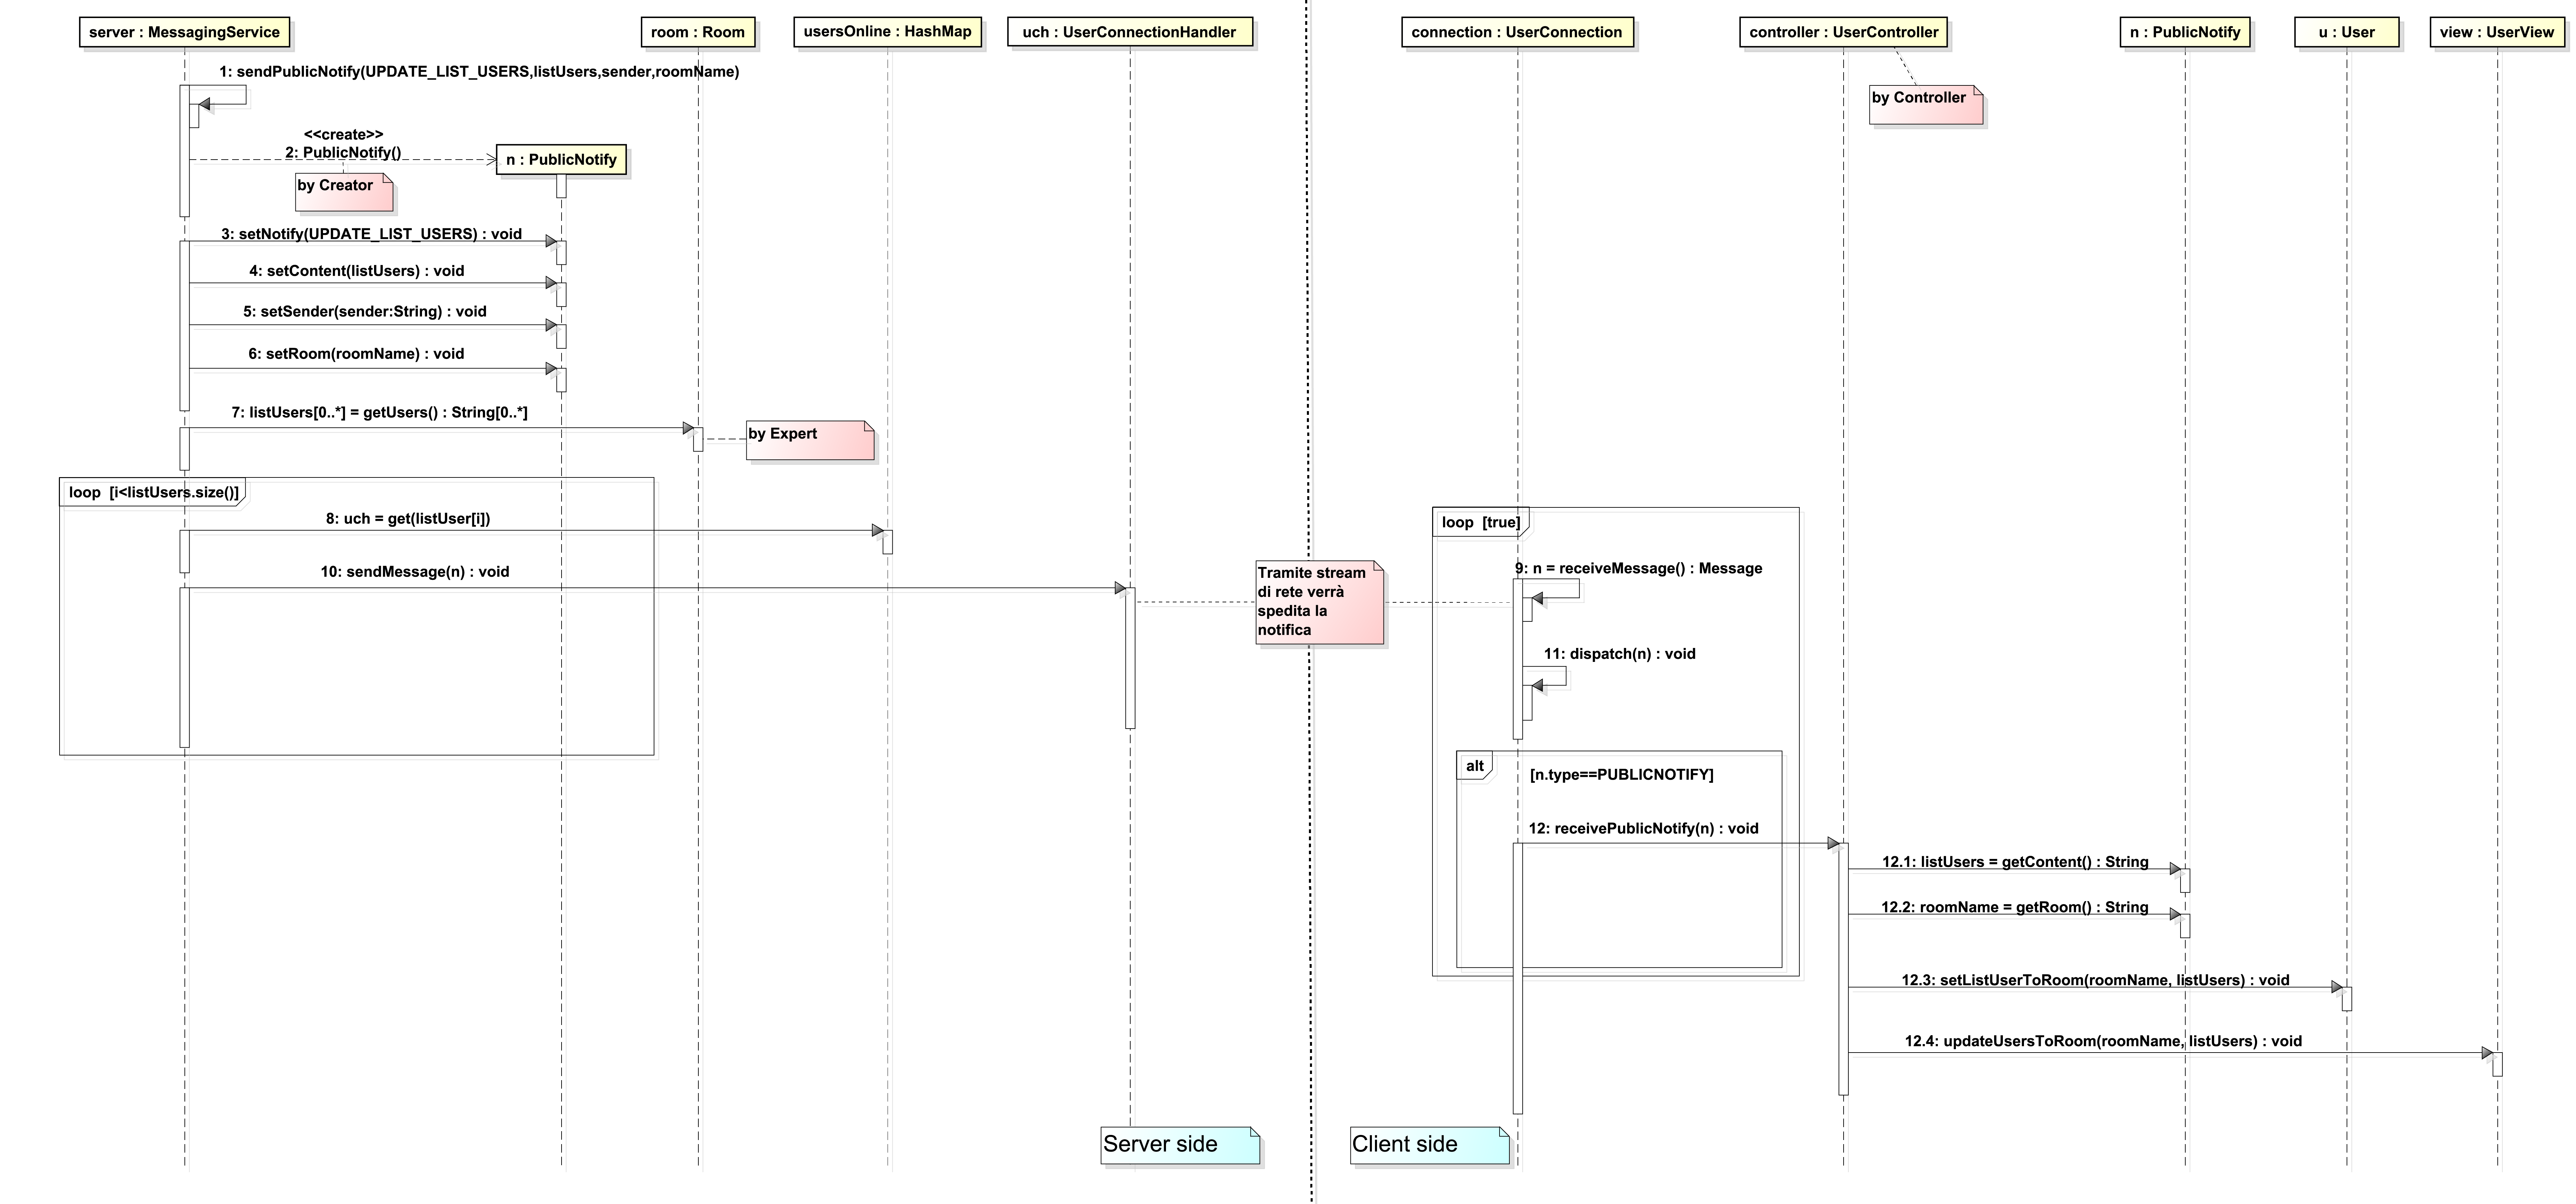
\includegraphics[scale=0.09]{image_astah/Iteration_1_DesignModel/UC2_AccessRoom_SSD_6_notifypublic.png}{\centering}
     \caption{SSD - OP6: notifypublic(updateList) del modello di dominio (figura \ref{fig_UC2_AR_SSD}) }
     \label{fig_UC2_SSD_AC_6} 
   \end{figure}
\end{frame}

